% ===========================================================
% ภาคผนวก
% ===========================================================
\appendiceschapter{}
\setcounter{chapter}{-1}

% =============================
% ภาคผนวก ก
% =============================
\appendiceschapter{การตั้งค่าที่ใช้ในการทดลอง}
\label{app:settings}

\renewcommand{\thesection}{ก.\arabic{section}}
\setcounter{section}{0}

\section{ค่าที่ใช้ในการปรับจูนและการเลือก Checkpoint}

ภาคผนวกนี้รวบรวมค่าที่ใช้จริงทั้งหมดไว้ในที่เดียว เพื่อให้ผู้ที่ต้องการทำซ้ำไม่ต้องไล่หาจากหลายบท
ตารางที่~\ref{tab:app_train} คือค่าของการปรับจูนและการเลือก Checkpoint
คอลัมน์ ``HairFastGAN'' และ ``Barbershop-FT'' แสดงค่าของแต่ละโมเดล
(Barbershop-FT คือ Barbershop ที่ปรับจูนแล้ว)
ตัวย่อในตาราง ได้แก่ IoU (Intersection over Union), ArcFace (Additive Angular Margin Loss),
MAE (Mean Absolute Error), MSE (Mean Squared Error), Adam (Adaptive Moment Estimation)
และ FFHQ (Flickr-Faces-HQ) ซึ่งเป็นชุดภาพใบหน้าที่ใช้ฝึก StyleGAN2
ถ้าค่าของสองโมเดลเหมือนกัน จะเขียนไว้ครั้งเดียวกลางแถว
จะเห็นว่าค่าเกือบทั้งหมดเหมือนกัน ต่างกันเฉพาะส่วนที่ปรับจูนและค่าสูญเสียส่วนเพิ่มที่ใช้กับ HairFastGAN เท่านั้น
ซึ่งเป็นไปตามหลักของโครงงานที่ต้องการให้ทั้งสองโมเดลอยู่ภายใต้เงื่อนไขเดียวกัน

\begin{table}[!tbp]
\centering
\caption{ค่าที่ใช้ในการปรับจูนและการเลือก Checkpoint}
\label{tab:app_train}
\small
\begin{tabular}{|L{4.2cm}|L{4.6cm}|L{4.6cm}|}
\hline
\textbf{รายการ} & \textbf{HairFastGAN} & \textbf{Barbershop-FT} \\ \hline
น้ำหนักเริ่มต้น & \multicolumn{2}{L{9.2cm}|}{น้ำหนักทางการของผู้พัฒนา (StyleGAN2 ฝึกบน FFHQ)} \\ \hline
ส่วนที่ปรับจูน & ชั้น Modulation ของ Blending Encoder และโมดูล PostProcess
& \texttt{convs[6:]} และ \texttt{to\_rgbs[3:]} ของ StyleGAN2 (ชั้น 64--1024 พิกเซล) \\ \hline
ส่วนที่ไม่ได้ปรับจูน & โมดูล Embedding (ผสม $F$ ด้วย $\alpha = 0.95$), Pose (หมุนเฉพาะภาพสีผม ไม่หมุนภาพทรงผม) และ Shape
& StyleGAN2 ชั้น 4--32 พิกเซล และขั้นค้นหารหัสตามค่าเดิม: II2S 1,100 รอบ, FS 250 รอบ, Alignment 140 + 100 รอบ, Blending 400 รอบ \\ \hline
ข้อมูล & \multicolumn{2}{L{9.2cm}|}{ชุดฝึก 150 ชุด, ชุดตรวจสอบ 9 ชุด, ชุดทดสอบ 10 ชุด ($1024 \times 1024$ พิกเซล)} \\ \hline
ฟังก์ชันสูญเสียหลัก & \multicolumn{2}{L{9.2cm}|}{$1.0\,L_{color} + 0.2\,L_{shape} + 0.1\,L_{id} + 5.0\,L_{protect} + 0.1\,L_{detail}$} \\ \hline
ค่าสูญเสียส่วนเพิ่ม & $0.5\,L_{color}(I_{pre}) + 0.1\,L_{shape}(I_{pre}) + 0.01\,\mathrm{MSE}(z, z_0)$ & ไม่มี \\ \hline
ตัวปรับค่า & \multicolumn{2}{L{9.2cm}|}{Adam ($\beta_1 = 0.9$, $\beta_2 = 0.999$) ตัดเกรเดียนต์ที่ขนาด 1.0} \\ \hline
Batch Size / Epoch / Updates & \multicolumn{2}{L{9.2cm}|}{1 / 30 / 4,500 ต่อ Trial} \\ \hline
อัตราการเรียนรู้ & \multicolumn{2}{L{9.2cm}|}{4 Trial ตามตารางที่~\ref{tab:trials}} \\ \hline
Seed & \multicolumn{2}{L{9.2cm}|}{3407} \\ \hline
สูตรคะแนนการเลือก & \multicolumn{2}{L{9.2cm}|}{$\frac{1}{2}(c/c_0 + e/e_0)$ เมื่อ $e = 1 - \mathrm{IoU}$} \\ \hline
ด่าน 5 ด่าน & \multicolumn{2}{L{9.2cm}|}{สีไม่แย่ลง, IoU ไม่ลดลง, ArcFace ลดได้ไม่เกิน 0.02,
MAE เพิ่มได้ไม่เกิน 0.01, Detail เพิ่มได้ไม่เกิน 0.091} \\ \hline
Checkpoint ที่เลือก & Trial B Epoch 24 (คะแนน 0.664) & Trial A Epoch 30 (คะแนน 0.841) \\ \hline
\end{tabular}
\par\vspace{3pt}{\footnotesize\raggedright หมายเหตุ: BS-FT (Barbershop-FT) = Barbershop ที่ปรับจูนแล้ว (Fine-tuned), II2S = Improved Image2StyleGAN, StyleGAN2 = Style-based Generative Adversarial Network รุ่นที่ 2, FFHQ = Flickr-Faces-HQ, MSE = Mean Squared Error, Adam = Adaptive Moment Estimation, IoU = Intersection over Union (สัดส่วนพื้นที่ผมที่ทับกัน), ArcFace = โมเดลจดจำใบหน้าที่ใช้วัดความเหมือนของใบหน้า, MAE = Mean Absolute Error (ค่าความคลาดเคลื่อนสัมบูรณ์เฉลี่ย)\par}

\end{table}

\section{ค่าที่ใช้ในขั้นขัดเกลาด้วย Diffusion}

ตารางที่~\ref{tab:app_diff} รวบรวมค่าของขั้นขัดเกลาทั้ง 4 ขั้นย่อย
โดย CFG คือ Classifier-Free Guidance และ UniPC คือ Unified Predictor-Corrector
แต่ละแถวคือหนึ่งขั้นย่อย คอลัมน์กลางคือค่าที่ใช้
และคอลัมน์ขวาคือเวลาเฉลี่ยต่อภาพของ HairFastGAN (HFG) จาก 8 ชุดภาพบน GPU A100
ขั้นนี้ใช้ค่าเดียวกันกับภาพจากทั้งสองโมเดล และไม่มีการฝึกเพิ่ม
ข้อความสั่งงานและข้อความเชิงลบฉบับเต็มอยู่ในหัวข้อที่~\ref{sec:diffusion}

\begin{table}[!tbp]
\centering
\caption{ค่าที่ใช้ในขั้นขัดเกลาด้วย Diffusion}
\label{tab:app_diff}
\small
\begin{tabular}{|L{3.4cm}|L{8.0cm}|c|}
\hline
\textbf{ขั้นย่อย} & \textbf{ค่าที่ใช้} & \textbf{เวลา (วินาที)} \\ \hline
1. หาบริเวณที่แก้ & SegFormer-B2, $M_{edit}$ = ผม $\cup$ ใบหน้า & 0.23 \\ \hline
2. Diffusion & Realistic Vision v5.1 (U-Net 4 ช่องสัญญาณ) ผ่าน Inpainting Pipeline ของ Diffusers, ความละเอียด 1024, Strength 0.15,
CFG 2.5, UniPC 30 ขั้น (ลบจริงประมาณ 4 ขั้น), Seed 3407 & 2.15 \\ \hline
3. เก็บพื้นหลัง & High-pass $\sigma = 1.2$ หักออก 0.5, น้ำหนัก 0.45, ระยะไล่น้ำหนัก 4--36 พิกเซล, จำกัด $\pm 4$ & 0.41 \\ \hline
4. Native Sharp & Unsharp Mask $\sigma = 0.75$ (0.75) และ $\sigma = 1.35$ (0.25),
หักออก 0.8, น้ำหนักผม 0.65 ใบหน้า 0.25, จำกัด $\pm 5$ & 0.36 \\ \hline
\textbf{รวม} & & \textbf{3.15} \\ \hline
\end{tabular}
\par\vspace{3pt}{\footnotesize\raggedright หมายเหตุ: SegFormer = Segmentation Transformer, CFG = Classifier-Free Guidance, UniPC = Unified Predictor-Corrector\par}

\end{table}

% =============================
% ภาคผนวก ข
% =============================
\appendiceschapter{แบบประเมินที่ใช้ในโครงงาน}
\label{app:survey}

\renewcommand{\thesection}{ข.\arabic{section}}
\setcounter{section}{0}

\section{แบบประเมินภาพแบบปกปิดชื่อโมเดล}

แบบประเมินนี้ใช้กับผู้ใช้ 41 คน แต่ละคนส่งภาพใบหน้าของตัวเอง เลือกภาพทรงผมและภาพสีผม
แล้วได้รับภาพผลลัพธ์ 4 ภาพจาก 4 ระบบ โดยไม่บอกว่าภาพใดมาจากระบบใด และสุ่มลำดับภาพใหม่สำหรับทุกคน
ผู้ใช้ตอบคำถามชุดเดียวกันกับทุกภาพ ตารางที่~\ref{tab:app_survey} คือคำถามและตัวเลือกคำตอบฉบับเต็ม
ข้อ 1--5 ตอบเป็นคะแนน 1--5 โดย 1 หมายถึงน้อยที่สุดและ 5 หมายถึงมากที่สุด
ส่วนข้อ 6 ให้เลือกช่วงเวลาหนึ่งช่วงจาก 6 ช่วง

\begin{table}[!htbp]
\centering
\caption{คำถามในแบบประเมินภาพแบบปกปิดชื่อโมเดล}
\label{tab:app_survey}
\small
\begin{tabular}{|c|L{8.0cm}|L{4.0cm}|}
\hline
\textbf{ข้อ} & \textbf{คำถาม} & \textbf{ตัวเลือกคำตอบ} \\ \hline
1 & ทรงผมใกล้เคียงกับภาพอ้างอิงมากเพียงใด & 1 2 3 4 5 \\ \hline
2 & สีผมตรงกับภาพอ้างอิงมากเพียงใด & 1 2 3 4 5 \\ \hline
3 & ภาพดูสมจริงและเป็นธรรมชาติมากเพียงใด & 1 2 3 4 5 \\ \hline
4 & ใบหน้ายังคงเหมือนตัวคุณมากเพียงใด & 1 2 3 4 5 \\ \hline
5 & คุณพึงพอใจกับภาพนี้สำหรับการใช้งานจริงมากเพียงใด & 1 2 3 4 5 \\ \hline
6 & หากต้องรอให้ระบบสร้างภาพที่มีคุณภาพเหมือนภาพนี้ คุณยินดีรอได้นานที่สุดเท่าใด
& น้อยกว่า 1 นาที, 1--5 นาที, 5--10 นาที, 10--20 นาที, 20--40 นาที, มากกว่า 40 นาที \\ \hline
\end{tabular}
\end{table}

\section{แบบประเมินหลังใช้งานเว็บแอปพลิเคชัน}

แบบประเมินนี้อยู่ในเว็บ LOOKLAB และเปิดได้จากปุ่ม ``แบบสอบถามประเมินผลลัพธ์'' หลังได้รับภาพ
ใช้เก็บข้อมูลการทดลองใช้งานจริง 100 ครั้งในบทที่ 4
ตารางที่~\ref{tab:app_web} แสดงหัวข้อทั้งหมดตามลำดับที่ปรากฏบนเว็บ
ข้อ 1--6 ให้คะแนน 1--5 ดาว โดยแต่ละระดับมีคำอธิบายกำกับ เช่น ข้อ 1 คือ
``ไม่ตรงเลย'' ``ตรงเล็กน้อย'' ``ตรงปานกลาง'' ``ตรงมาก'' และ ``ตรงตาม reference มากที่สุด''
(คำว่า reference บนเว็บหมายถึงภาพอ้างอิง)
ในข้อ 1 และ 2 ระบบจะแสดงชื่อทรงผมและสีผมที่ผู้ใช้เลือกไว้ในคำถามด้วย
ถ้าผู้ใช้เลือกทรงผมต้นฉบับหรือสีธรรมชาติ คำถามจะเปลี่ยนเป็นการประเมินว่าระบบคงทรงหรือสีเดิมไว้ได้ดีเพียงใด
นอกจากคำตอบของผู้ใช้ ระบบยังบันทึกเวลารอจริงของแต่ละครั้งโดยอัตโนมัติ
และจะแนบรูปต้นฉบับกับรูปผลลัพธ์ไปกับคำตอบเฉพาะเมื่อผู้ใช้ติ๊กยินยอมเท่านั้น
ภาพที่~\ref{fig:app_feedback_done} คือหน้าที่ผู้ใช้เห็นหลังส่งแบบประเมินเรียบร้อยแล้ว

\begin{table}[!htbp]
\centering
\caption{หัวข้อในแบบประเมินหลังใช้งานเว็บแอปพลิเคชัน LOOKLAB}
\label{tab:app_web}
\small
\begin{tabular}{|c|L{7.6cm}|L{4.4cm}|}
\hline
\textbf{ข้อ} & \textbf{หัวข้อ} & \textbf{ตัวเลือกคำตอบ} \\ \hline
-- & คุณอยู่ในช่วงอายุใด (จำเป็นต้องตอบ) & ต่ำกว่า 18, 18--24, 25--34, 35--44, 45--54 และ 55 ปีขึ้นไป \\ \hline
1 & ทรงผมในภาพผลลัพธ์ตรงตาม reference แค่ไหน & 1--5 ดาว \\ \hline
2 & สีผมในภาพผลลัพธ์ตรงตาม reference แค่ไหน & 1--5 ดาว \\ \hline
3 & ใบหน้าในภาพผลลัพธ์เหมือนใบหน้าต้นฉบับแค่ไหน & 1--5 ดาว \\ \hline
4 & คุณพอใจกับระยะเวลาที่รอผลลัพธ์แค่ไหน & 1--5 ดาว \\ \hline
5 & คุณพอใจกับผลลัพธ์โดยรวมมากแค่ไหน & 1--5 ดาว \\ \hline
6 & คุณพอใจกับการใช้งานเว็บไซต์นี้มากแค่ไหน & 1--5 ดาว \\ \hline
-- & ข้อเสนอแนะเพิ่มเติม (ไม่บังคับ) & เขียนตอบอิสระ \\ \hline
-- & ยินยอมให้เก็บรูปต้นฉบับและรูปผลลัพธ์เพื่อประเมินและปรับปรุงระบบ & เลือกหรือไม่เลือกก็ได้ \\ \hline
\end{tabular}
\end{table}

\begin{figure}[!htbp]
\centering
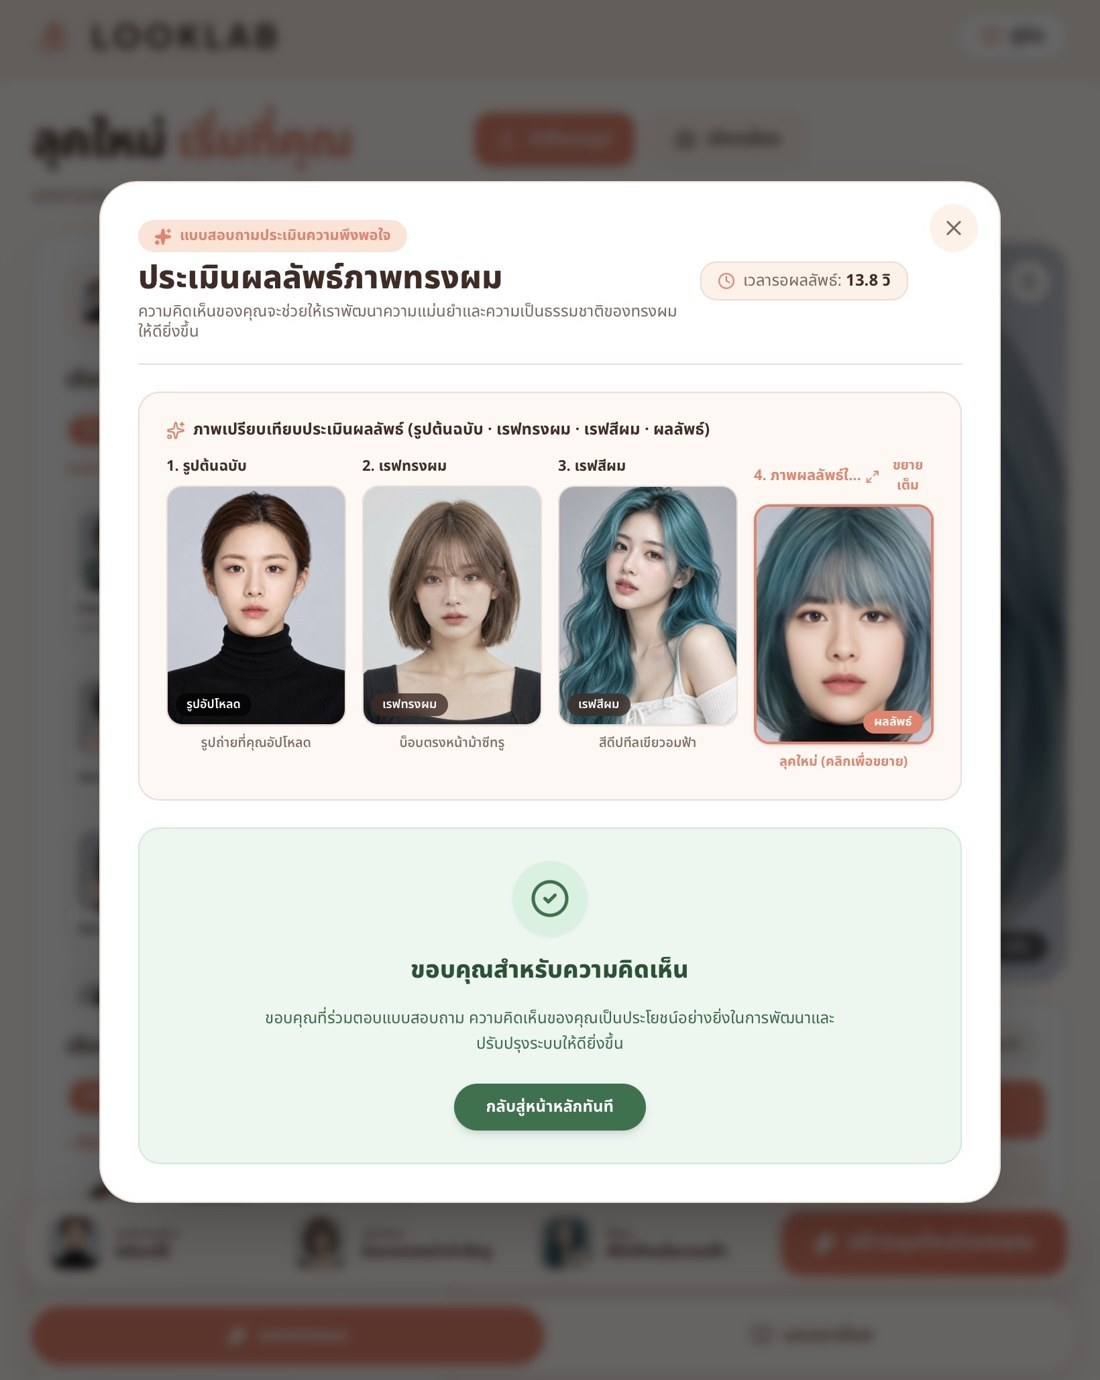
\includegraphics[width=0.55\textwidth]{images/looklab_feedback_done.jpg}
\caption{หน้าหลังส่งแบบประเมินบนเว็บ LOOKLAB}
\label{fig:app_feedback_done}
\end{figure}

% =============================
% ภาคผนวก ค
% =============================
\appendiceschapter{ผลการทดลองเพิ่มเติม}
\label{app:extra}

\renewcommand{\thesection}{ค.\arabic{section}}
\setcounter{section}{0}

\section{ตัวอย่างผลลัพธ์ของโมเดลตั้งต้น}

ก่อนเริ่มปรับจูน ผู้วิจัยรันโมเดลตั้งต้นทั้งสองตัวกับภาพของผู้วิจัย เพื่อดูว่าแต่ละตัวมีจุดอ่อนอะไร
ภาพที่~\ref{fig:app_base} เป็นตัวอย่างหนึ่งชุด แถวบนคือภาพนำเข้า ได้แก่ (ก) ภาพใบหน้า
(ข) ภาพอ้างอิงทรงผม และ (ค) ภาพอ้างอิงสีผม แถวล่างคือผลของ (ง) HairFastGAN และ (จ) Barbershop
ทั้งสองโมเดลวางทรงหน้าม้าและสีแดงได้ใกล้ภาพอ้างอิง แต่ผลของ HairFastGAN มีผมเรียบเกินไปจนสีดูเป็นปื้น
ส่วนผลของ Barbershop มีเส้นผมมากกว่า แต่หน้าม้าดูไม่เรียบร้อยและสีไม่สม่ำเสมอ
ข้อสังเกตจากภาพชุดนี้เป็นจุดเริ่มต้นของการออกแบบฟังก์ชันสูญเสียด้านสีและด้านรายละเอียดผมในบทที่ 3

\begin{figure}[!htbp]
\centering
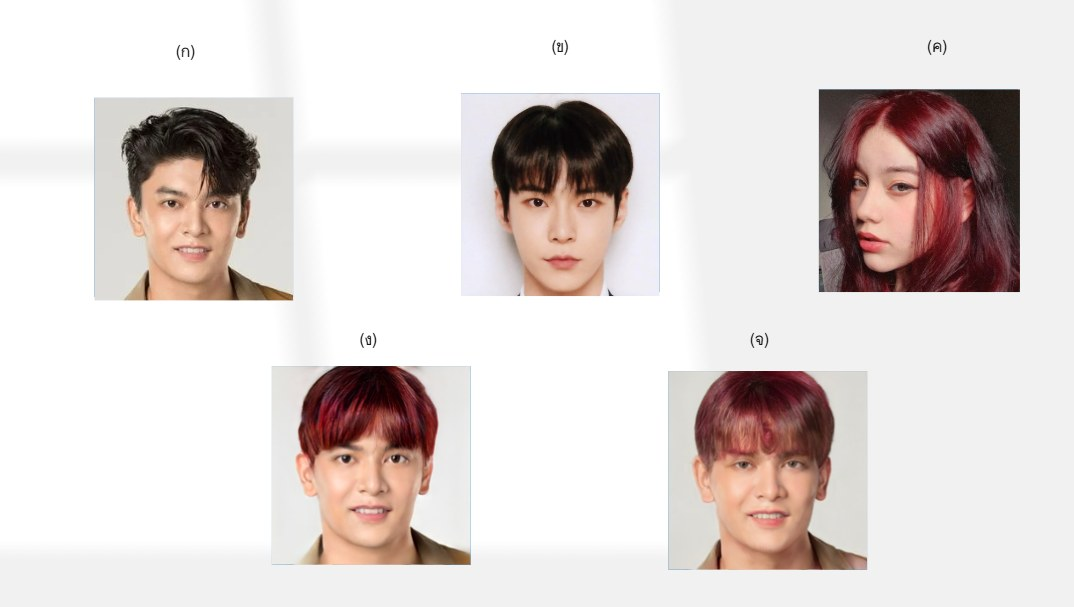
\includegraphics[width=0.85\textwidth]{images/test1.jpg}
\caption{ตัวอย่างภาพนำเข้าและผลลัพธ์ของ HairFastGAN และ Barbershop ก่อนปรับจูน}
\label{fig:app_base}
\end{figure}

\section{การเปรียบเทียบข้อความสั่งงานของ Diffusion}

ข้อความสั่งงาน (Prompt) มีผลต่อสิ่งที่ Diffusion วาดเพิ่ม ผู้วิจัยจึงลองข้อความ 6 แบบ (P1--P6)
กับภาพจากทั้งสองโมเดลก่อนเลือกข้อความที่ใช้จริง
ภาพที่~\ref{fig:app_prompt1} และ~\ref{fig:app_prompt2} เป็นตัวอย่างสองชุด
แถวบนของแต่ละภาพคือภาพนำเข้า 3 ภาพ แถวกลางคือผลของ HairFastGAN ก่อนผ่าน Diffusion (ซ้ายสุด)
ตามด้วยผลหลังผ่าน Diffusion ด้วยข้อความที่ 1--6 และแถวล่างคือผลแบบเดียวกันของ Barbershop
เมื่อดูด้วยตา ความต่างระหว่างข้อความแต่ละแบบมีน้อย เพราะใช้ความแรงต่ำ
ความต่างหลักอยู่ที่ความชัดของเส้นผมและความเข้มของสีผมเล็กน้อย
ส่วนทรงผม ใบหน้า และพื้นหลังแทบไม่เปลี่ยนในทุกข้อความ

\begin{figure}[!htbp]
\centering
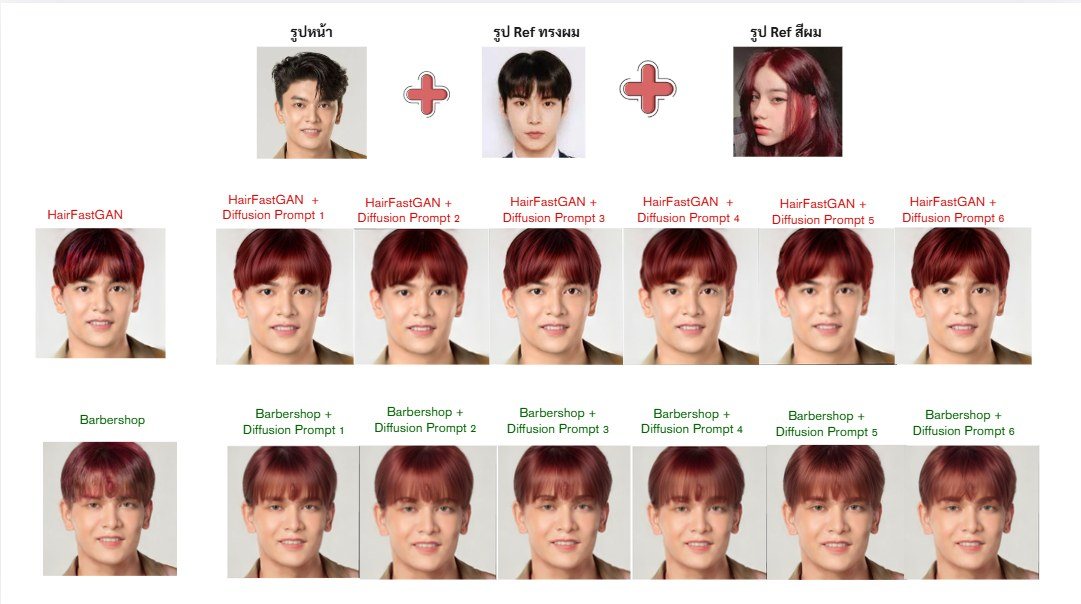
\includegraphics[width=\textwidth]{images/test2.jpg}
\caption{ผลของข้อความสั่งงาน 6 แบบกับภาพจาก HairFastGAN และ Barbershop (ตัวอย่างที่ 1)}
\label{fig:app_prompt1}
\end{figure}

\begin{figure}[!htbp]
\centering
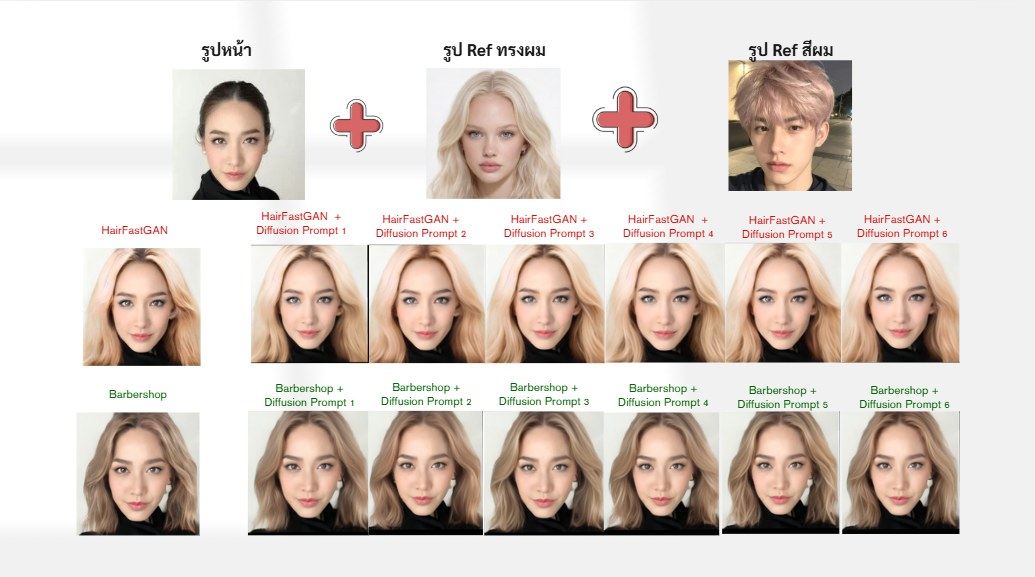
\includegraphics[width=\textwidth]{images/test3.jpg}
\caption{ผลของข้อความสั่งงาน 6 แบบกับภาพจาก HairFastGAN และ Barbershop (ตัวอย่างที่ 2)}
\label{fig:app_prompt2}
\end{figure}

ภาพที่~\ref{fig:app_prompt_metric} วัดผลเดียวกันเป็นตัวเลข แถวบนคือ HairFastGAN และแถวล่างคือ Barbershop
แต่ละคอลัมน์คือตัวชี้วัดหนึ่งตัว ได้แก่ SSIM (Structural Similarity Index), อัตราส่วนสัญญาณสูงสุดต่อสัญญาณรบกวน
(Peak Signal-to-Noise Ratio: PSNR), ความคล้ายของทรงผมที่วัดด้วย CLIP (CLIP-Shape)
และความคล้ายของสีผมที่วัดด้วย CLIP (CLIP-Color) ทุกตัวยิ่งสูงยิ่งดี
แท่งสีจางคือภาพก่อนผ่าน Diffusion (Base) แท่งสีกลางคือข้อความ P1--P5 และแท่งสีเข้มคือข้อความ P6

ผลที่เห็นคือทุกข้อความทำให้ SSIM สูงกว่าภาพก่อนผ่าน Diffusion
(HairFastGAN จาก 0.3827 เป็น 0.390--0.395 และ Barbershop จาก 0.3794 เป็น 0.387--0.391)
ส่วน PSNR, CLIP-Shape และ CLIP-Color เปลี่ยนน้อยมาก ส่วนใหญ่ต่างกันไม่ถึง 0.01
ข้อความ P6 เป็นข้อความเดียวที่ทำให้ CLIP-Shape ของ HairFastGAN สูงกว่าก่อนผ่าน Diffusion (0.6545 เทียบกับ 0.6535)
และให้ค่าที่ไม่ต่ำกว่าข้อความอื่นมากในทุกตัวชี้วัด
ข้อสรุปจากการทดลองนี้คือ เมื่อใช้ความแรงต่ำ การเลือกข้อความสั่งงานมีผลต่อผลลัพธ์ไม่มาก
และในการทดลองนี้ Diffusion แทบไม่เปลี่ยนทรงและสีผมเมื่อวัดด้วย CLIP ซึ่งสอดคล้องกับคะแนนทรงและสีผมจากผู้ใช้ในบทที่ 4
แม้กรณีศึกษาเชิงตัวเลขในบทที่ 4 จะพบว่าสีผมของ HairFastGAN เพี้ยนจากเป้าหมายเล็กน้อยหลังผ่าน Diffusion

\begin{figure}[!htbp]
\centering
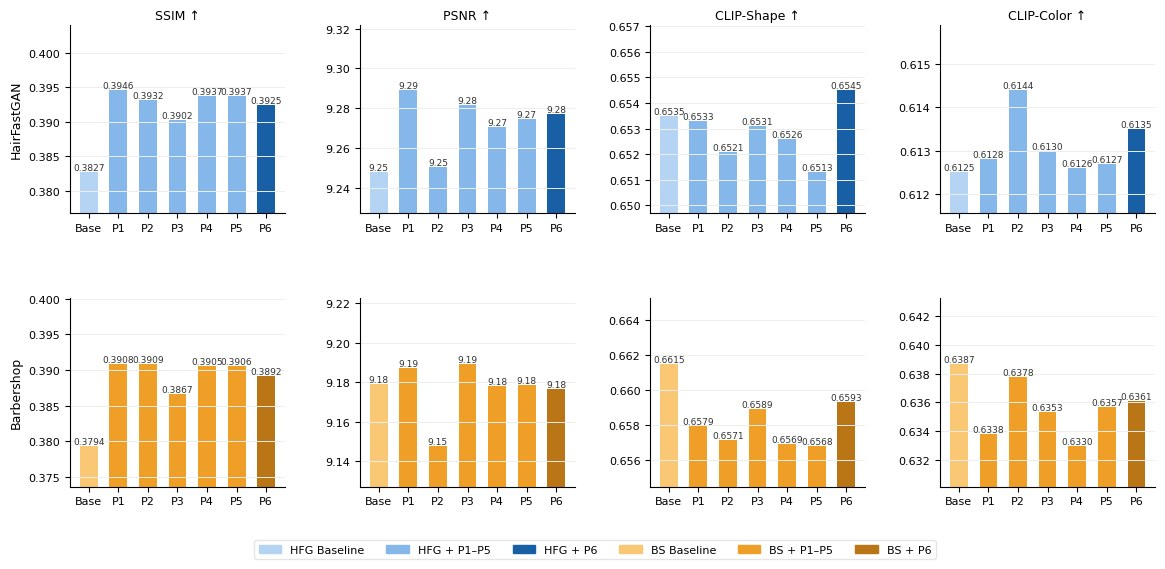
\includegraphics[width=\textwidth]{images/fig_prompt_comparison.jpg}
\caption{ตัวชี้วัดของภาพก่อนผ่าน Diffusion (Base) และหลังผ่านด้วยข้อความ P1--P6}
\label{fig:app_prompt_metric}
\par\vspace{3pt}{\footnotesize\raggedright หมายเหตุ: P1--P6 = ข้อความสั่งงาน (Prompt) แบบที่ 1 ถึง 6, HFG = HairFastGAN, BS = Barbershop ก่อนปรับจูน, SSIM = Structural Similarity Index (ดัชนีความคล้ายเชิงโครงสร้าง), PSNR = Peak Signal-to-Noise Ratio, CLIP = Contrastive Language-Image Pre-training\par}
\end{figure}

% =============================
% ภาคผนวก ง
% =============================
\appendiceschapter{คู่มือการใช้งานเว็บแอปพลิเคชัน LOOKLAB}
\label{app:manual}

\renewcommand{\thesection}{ง.\arabic{section}}
\setcounter{section}{0}
\section{การเข้าใช้งาน}

LOOKLAB ใช้งานผ่านเว็บเบราว์เซอร์ได้ทันทีโดยไม่ต้องติดตั้งโปรแกรม
เข้าได้ที่ \url{https://looklab2.vercel.app/} หรือสแกนคิวอาร์โค้ดในภาพที่~\ref{fig:app_qr}
เมื่อเปิดเว็บครั้งแรก ระบบจะแสดงหน้าต่างคู่มือดังภาพที่~\ref{fig:app_guide}
ซึ่งมี 4 แท็บ คือ ขั้นตอนเริ่มใช้ เทคนิคเตรียมรูป คำแนะนำทรงผมและสีผม และคำถามที่พบบ่อย
ผู้ใช้กด ``เข้าใจแล้ว'' เพื่อเริ่มใช้งาน และเปิดคู่มือนี้อีกครั้งได้จากปุ่ม ``คู่มือ'' ที่มุมขวาบน

\begin{figure}[!htbp]
\centering

\includegraphics[width=0.3\textwidth]{images/looklab_qr.png}
\caption{คิวอาร์โค้ดสำหรับเข้าเว็บแอปพลิเคชัน LOOKLAB}
\label{fig:app_qr}
\end{figure}

\begin{figure}[!htbp]
\centering
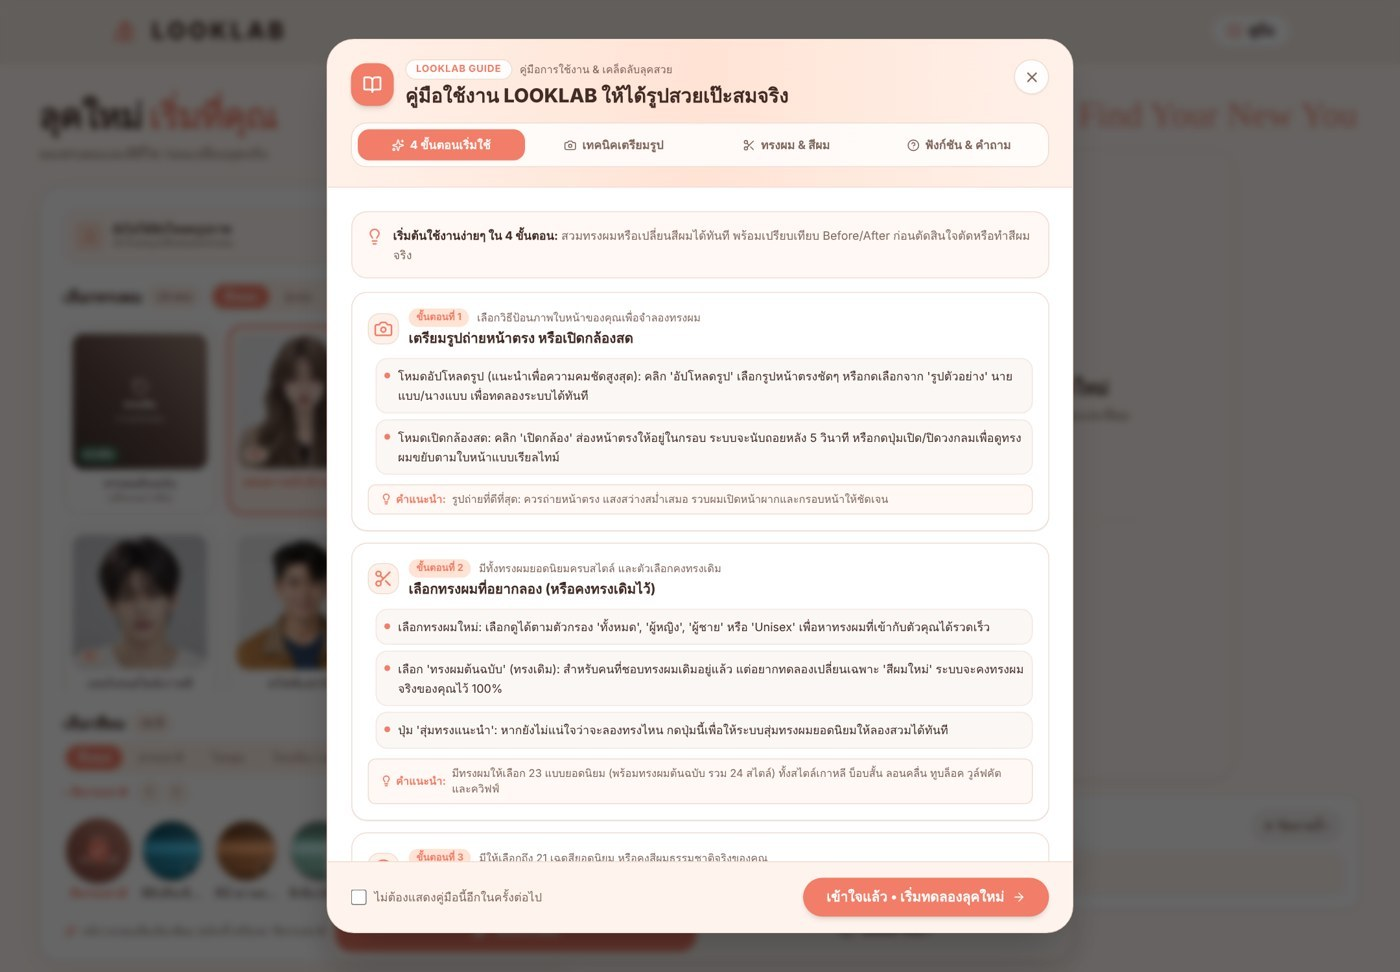
\includegraphics[width=0.8\textwidth]{images/looklab_guide.jpg}
\caption{หน้าต่างคู่มือการใช้งานที่แสดงเมื่อเปิดเว็บครั้งแรก}
\label{fig:app_guide}
\end{figure}

\section{ขั้นตอนการใช้งานโหมดอัปโหลดรูป}

หน้าหลักของ LOOKLAB แบ่งเป็น 3 ส่วน ด้านซ้ายเป็นแผงสำหรับเลือกทรงผมและสีผม
ด้านขวาเป็นพื้นที่แสดงรูปของผู้ใช้และภาพผลลัพธ์
และด้านล่างเป็นแถบสรุปที่แสดงรูป ทรงผม และสีผมที่เลือกอยู่ พร้อมปุ่ม ``สร้างลุคใหม่ของคุณ''
ผู้ใช้เลือกใช้งานได้ 2 โหมด คือ โหมดอัปโหลดรูป ซึ่งให้ภาพผลลัพธ์คุณภาพสูง
และโหมดกล้องสด ซึ่งแสดงทรงผมใหม่บนภาพจากกล้องและขยับตามใบหน้า
โหมดอัปโหลดรูปมี 7 ขั้นตอน ดังนี้

\textbf{ขั้นที่ 1 ใส่รูปใบหน้า} มี 3 วิธีให้เลือก
วิธีแรกคือกดปุ่ม ``อัปโหลดรูปภาพ'' กลางพื้นที่ด้านขวา หรือปุ่ม ``อัปโหลดรูป'' ด้านบน ดังภาพที่~\ref{fig:1}
แล้วเลือกรูปหน้าตรงจากเครื่อง หรือลากไฟล์มาวางในพื้นที่ด้านขวา
วิธีที่สองคือกด ``เปิดกล้อง'' เพื่อถ่ายรูปจากกล้อง ซึ่งอธิบายไว้ในหัวข้อที่~\ref{sec:camera}
และวิธีที่สามคือกดรูปตัวอย่าง ``ผู้หญิง'' หรือ ``ผู้ชาย'' เพื่อทดลองระบบโดยไม่ต้องใช้รูปของตัวเอง
ถ้าเคยใช้งานมาก่อน จะมีกล่อง ``ใช้รูปเดิมของคุณ'' อยู่ใต้ปุ่มอัปโหลด ให้กด ``เลือกรูปนี้''
หรือกด ``ใช้รูปเดิม'' ที่แผงด้านซ้าย รูปเดิมนี้บันทึกไว้เฉพาะในเครื่องของผู้ใช้เท่านั้น คนอื่นมองไม่เห็น

\begin{figure}[!htbp]
\centering
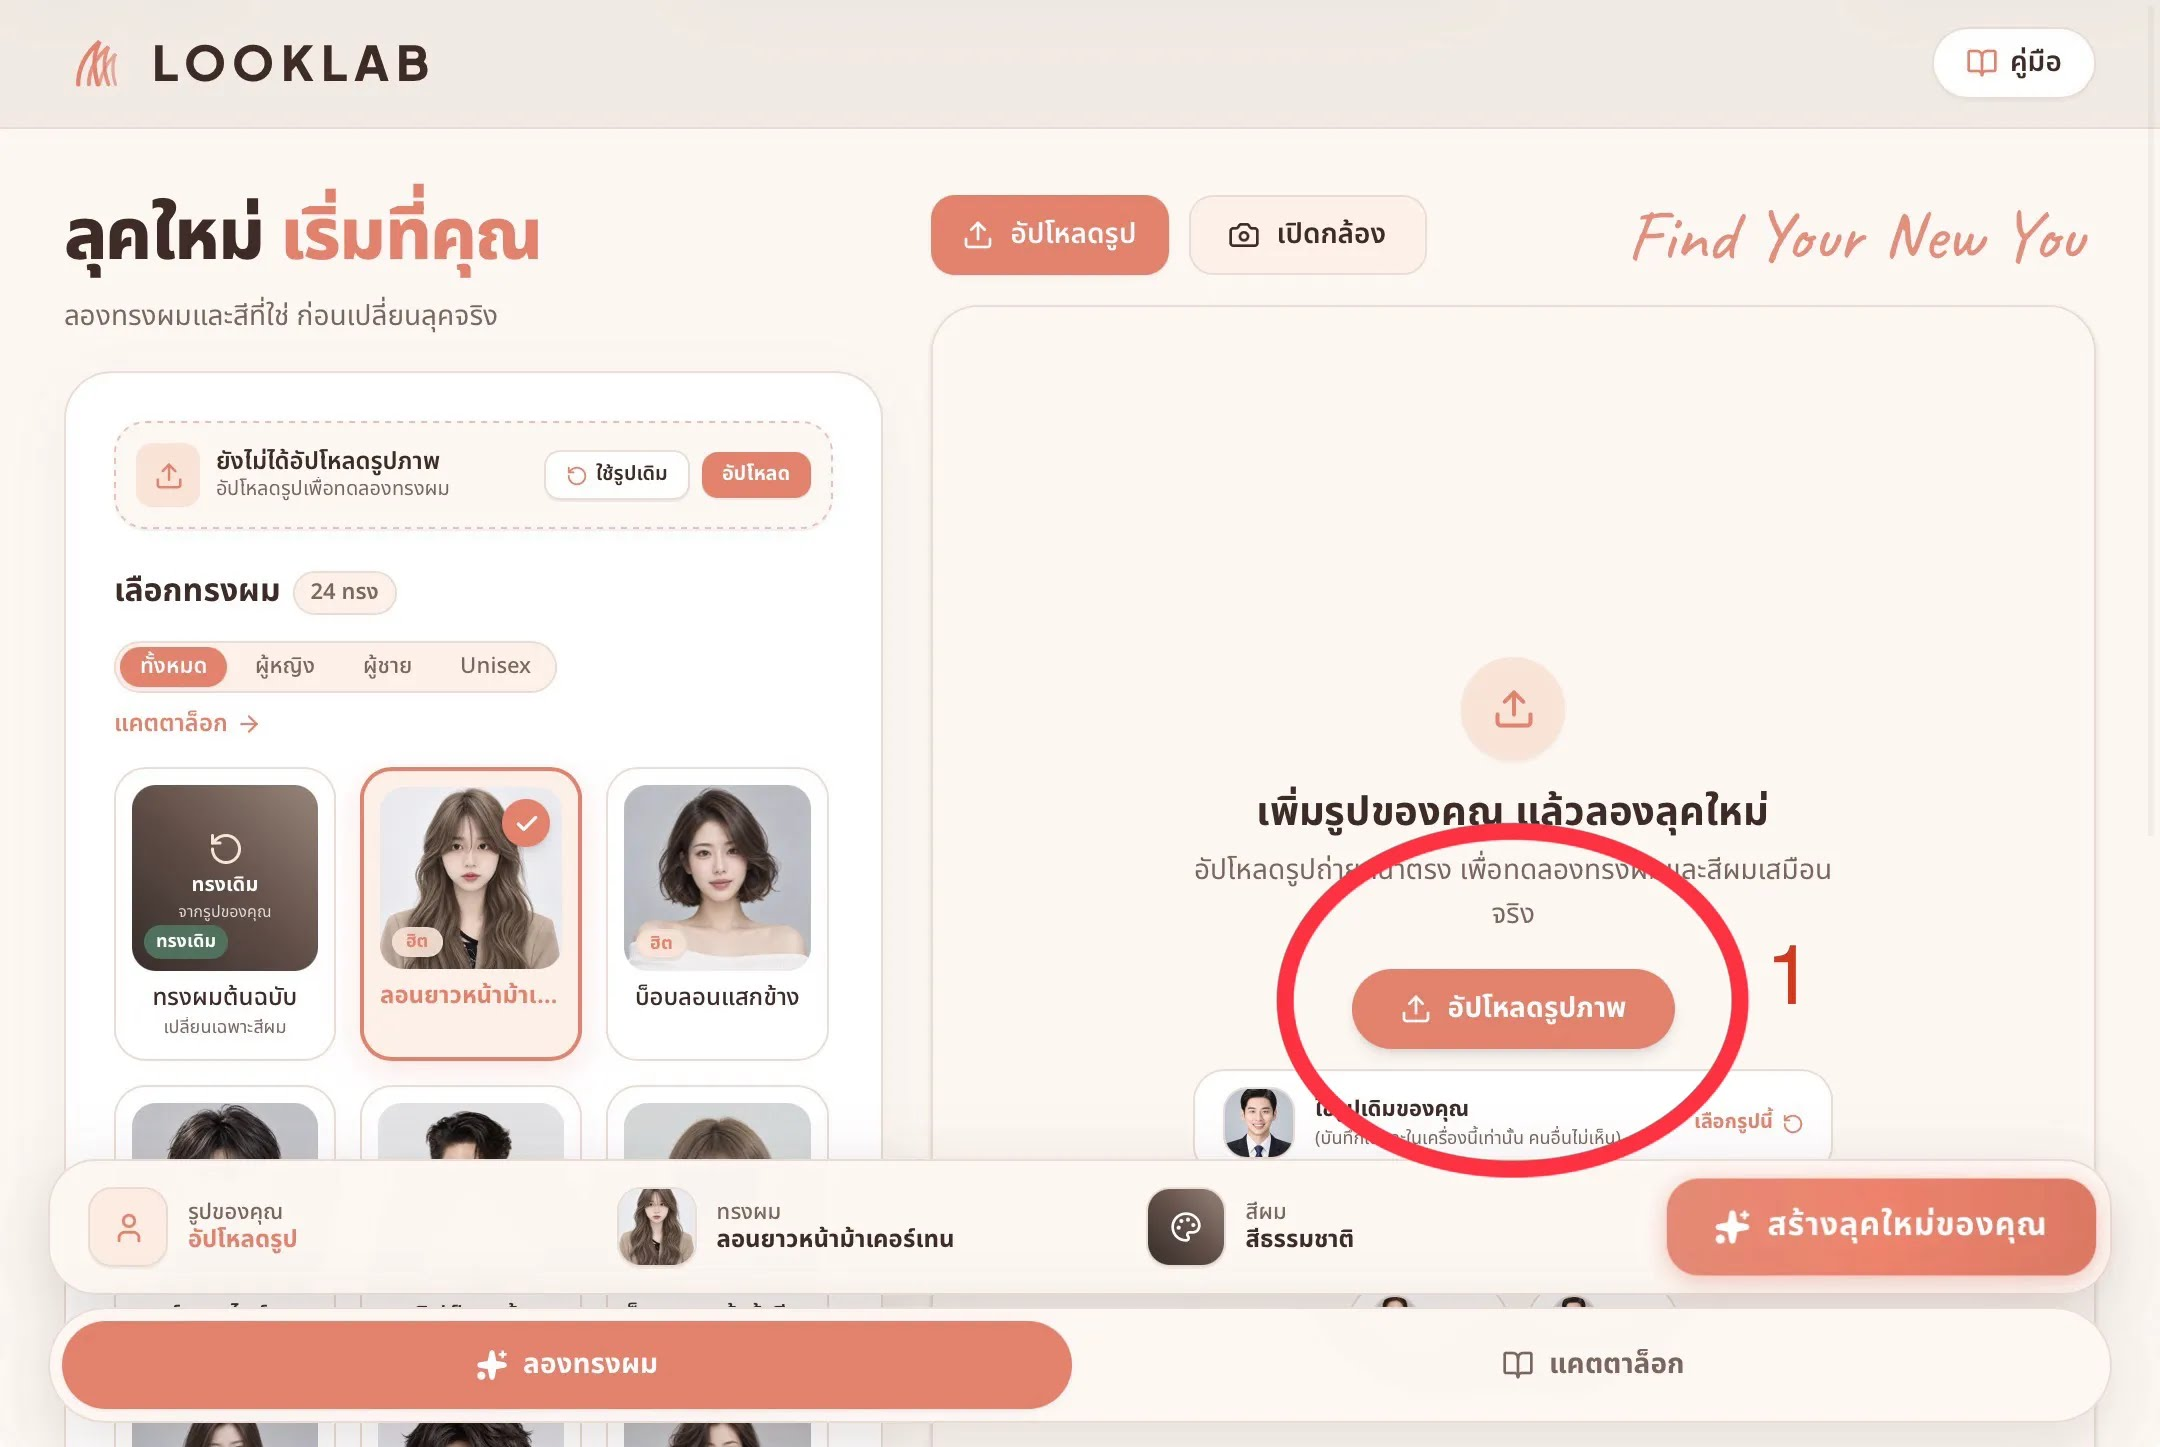
\includegraphics[width=0.9\textwidth]{images/1.jpeg}
\caption{หน้าหลักก่อนใส่รูปและปุ่มอัปโหลดรูปภาพ}
\label{fig:1}
\end{figure}

\textbf{ขั้นที่ 2 ตรวจใบหน้าและเลือกทรงผม}
เมื่อระบบพบใบหน้า จะแสดงกรอบวงรีสีเขียวรอบใบหน้า
และสถานะ ``รูปของคุณ'' ในแถบด้านล่างจะเปลี่ยนเป็น ``พร้อมใช้''
จากนั้นเลือกทรงผมจากแผง ``เลือกทรงผม'' ด้านซ้าย ซึ่งมีทั้งหมด 24 ทรง
กรองได้ด้วยแท็บ ``ทั้งหมด'' ``ผู้หญิง'' ``ผู้ชาย'' และ ``Unisex''
ทรงที่มีป้าย ``ฮิต'' คือทรงยอดนิยม
ทรงที่เลือกอยู่จะมีกรอบสีส้มพร้อมเครื่องหมายถูก
และชื่อทรงจะแสดงในช่อง ``ทรงผม'' ของแถบด้านล่าง ดังภาพที่~\ref{fig:2}
ถ้าต้องการเปลี่ยนเฉพาะสีผม ให้เลือกการ์ดแรก ``ทรงผมต้นฉบับ'' ระบบจะคงทรงผมเดิมไว้
และถ้าอยากดูภาพใหญ่ก่อนตัดสินใจ ให้กด ``แคตตาล็อก''

\begin{figure}[H]
\centering
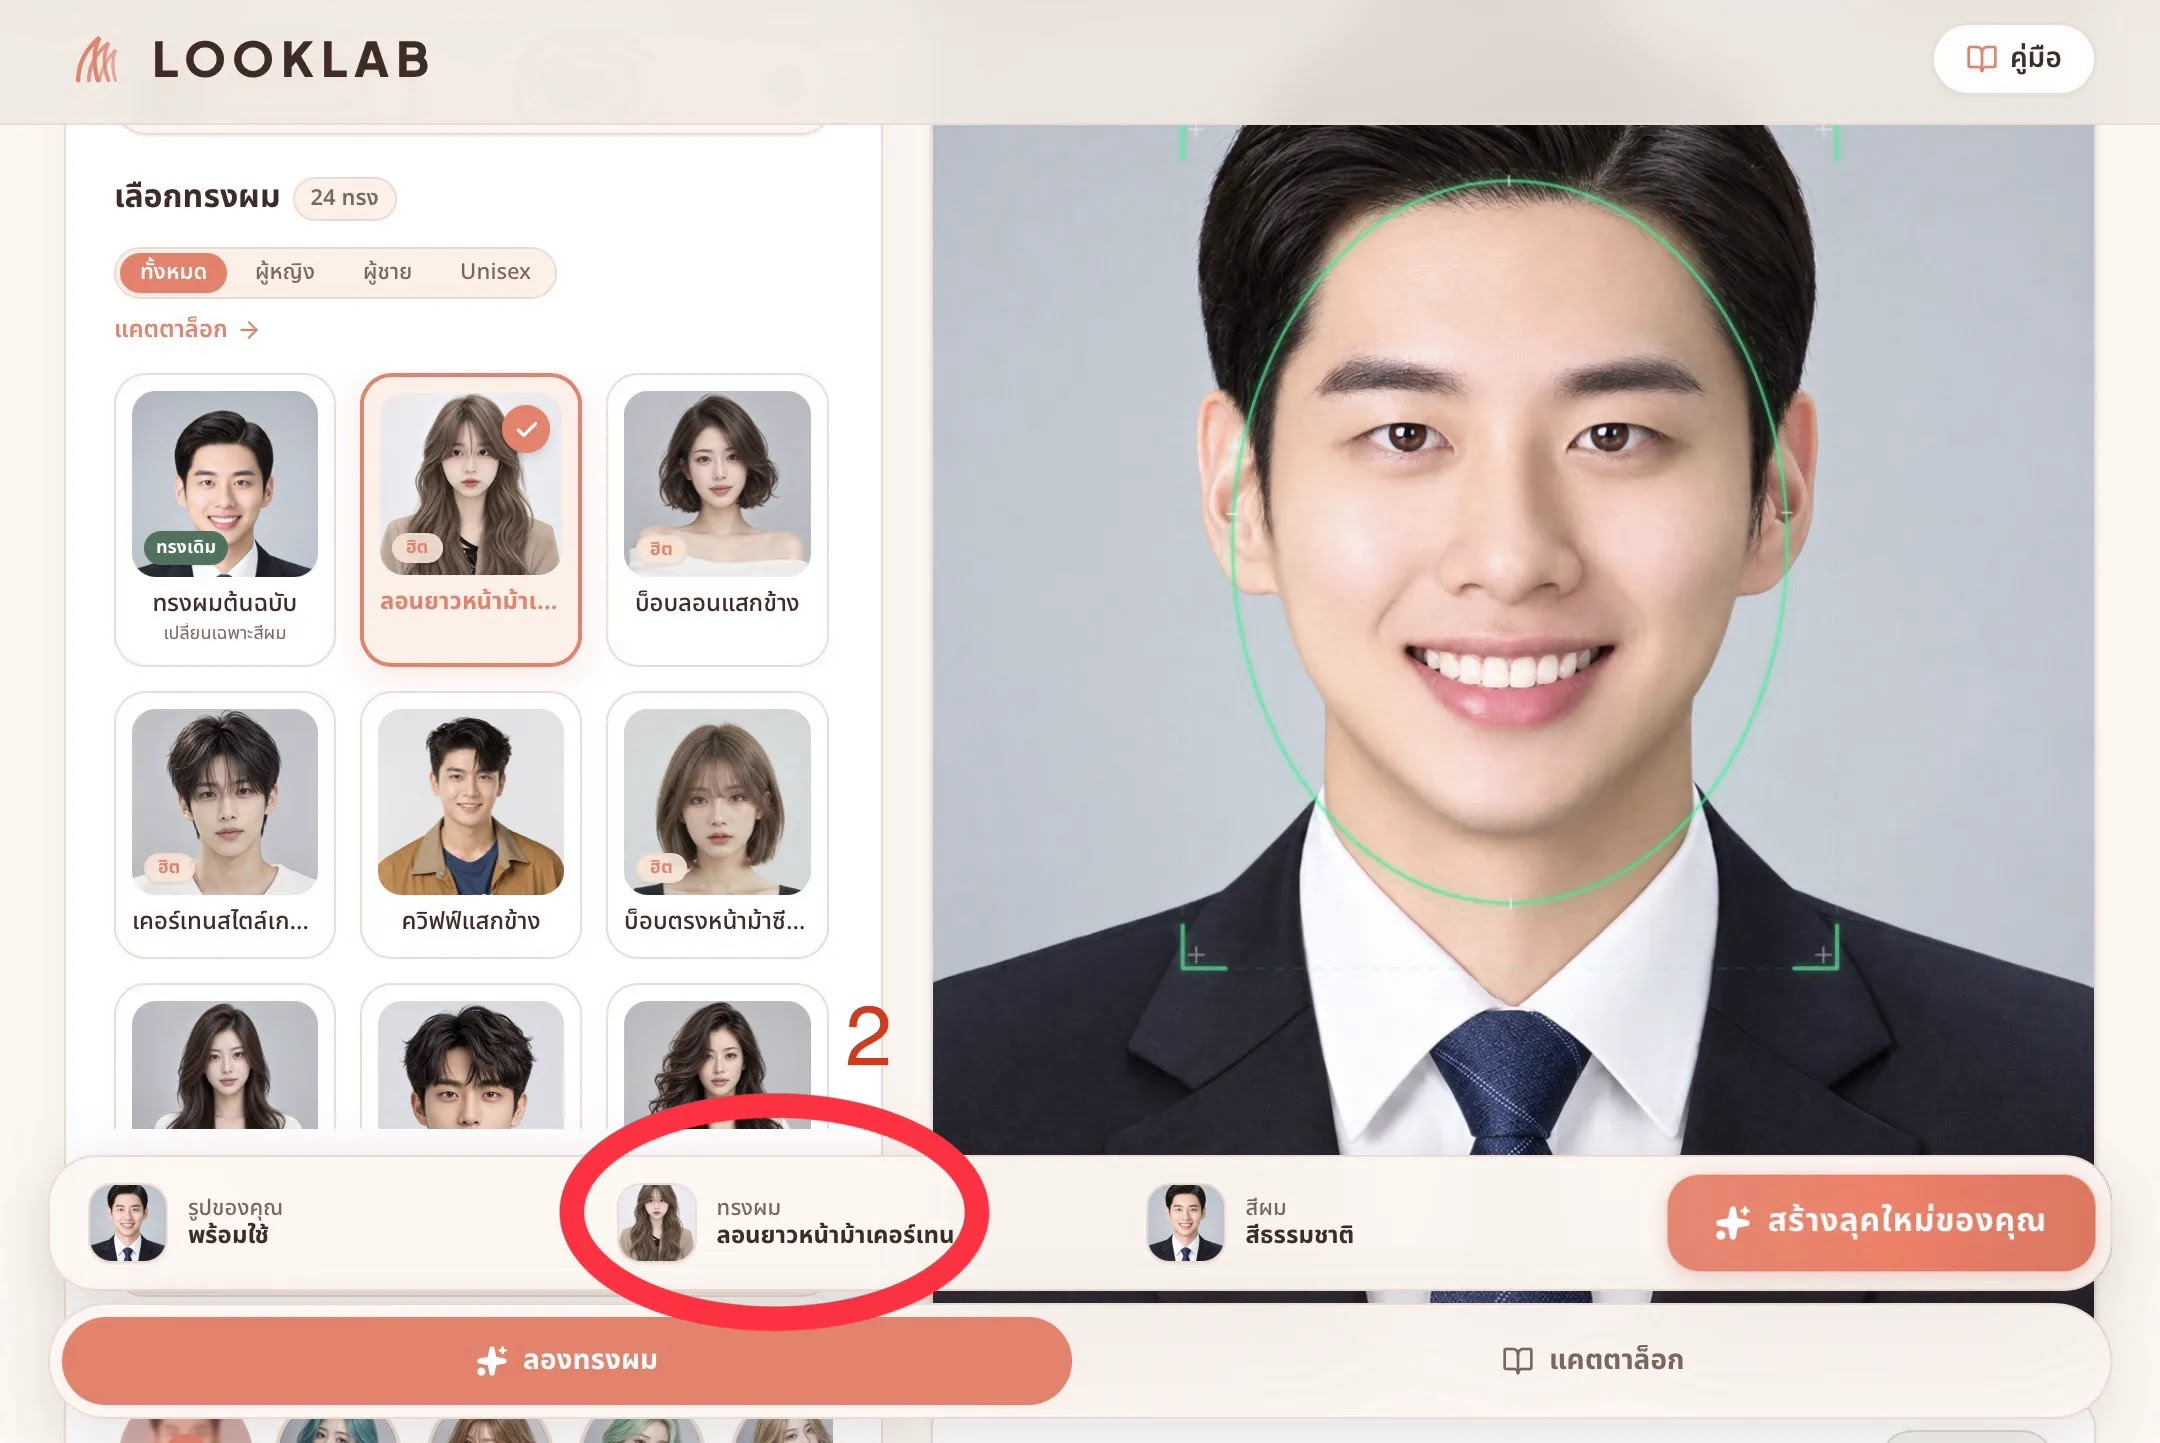
\includegraphics[width=0.9\textwidth]{images/2.jpeg}
\caption{การตรวจพบใบหน้าและการเลือกทรงผม}
\label{fig:2}
\end{figure}

\textbf{ขั้นที่ 3 เลือกสีผม}
เลื่อนแผงด้านซ้ายลงมาที่ส่วน ``เลือกสีผม'' ซึ่งมีทั้งหมด 28 สี
กรองตามโทนได้ด้วยแท็บ ``ทั้งหมด'' ``ธรรมชาติ'' ``โทนอุ่น'' ``โทนเย็น / แอช'' และ ``แฟชั่น / พาสเทล''
และเลื่อนดูสีอื่นได้ด้วยลูกศรซ้ายขวา คลิกที่วงกลมเพื่อเลือกสี
ชื่อสีที่เลือกจะแสดงในช่อง ``สีผม'' ของแถบด้านล่าง
ถ้าต้องการเปลี่ยนเฉพาะทรงผม ให้เลือก ``สีธรรมชาติ''
หรือคลิกซ้ำที่สีที่เลือกอยู่เพื่อกลับไปใช้สีผมเดิมของรูปต้นฉบับ

\textbf{ขั้นที่ 4 สร้างภาพ}
ตรวจสอบรูป ทรงผม และสีผมในแถบด้านล่างอีกครั้ง
แล้วกดปุ่ม ``สร้างลุคใหม่ของคุณ'' ทางขวาของแถบ ดังภาพที่~\ref{fig:3-4}

\begin{figure}[H]
\centering
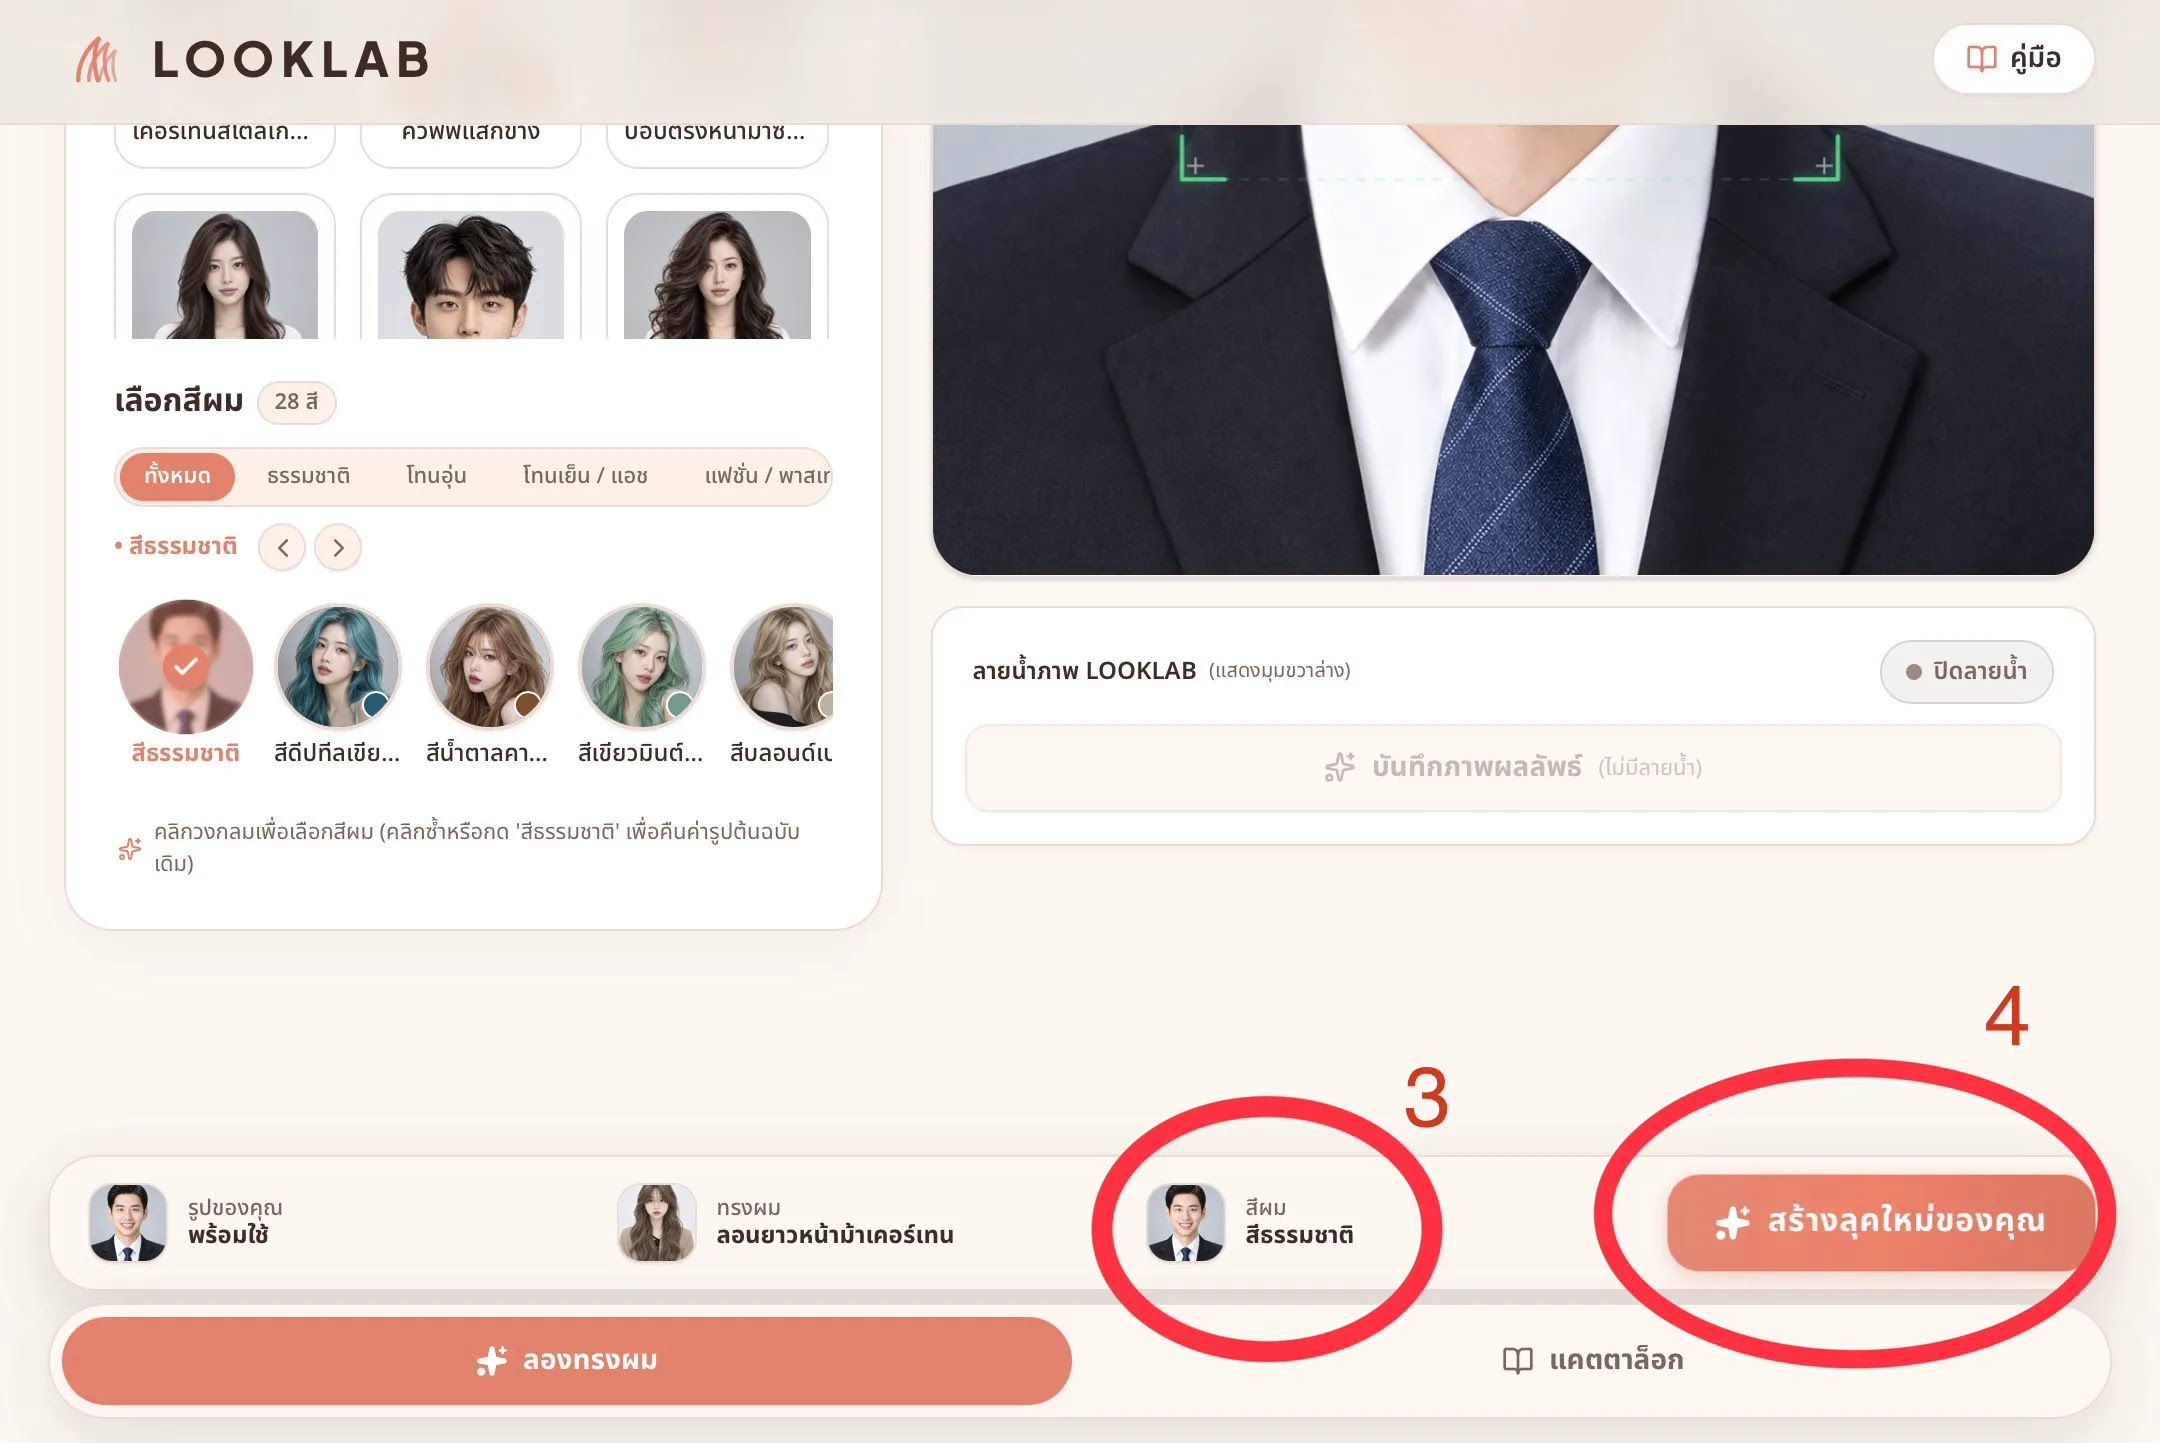
\includegraphics[width=0.9\textwidth]{images/3-4.jpeg}
\caption{การเลือกสีผมและปุ่มสร้างลุคใหม่ของคุณ}
\label{fig:3-4}
\end{figure}

\textbf{ขั้นที่ 5 รอระบบประมวลผล}
ระบบจะแสดงหน้าต่าง ``กำลังสร้างลุคทรงผมใหม่'' พร้อมรูปต้นฉบับ เวลาประมวลผลที่ผ่านไป สถานะการทำงาน
และภาพอ้างอิงทรงผมกับภาพอ้างอิงสีผมที่เลือก ดังภาพที่~\ref{fig:5}
จากการทดลองใช้งานจริง ขั้นนี้ใช้เวลาประมาณ 15 วินาที (ค่ามัธยฐาน 14.9 วินาที)
ระหว่างรอไม่ควรปิดหรือรีเฟรชหน้าเว็บ
ถ้าต้องการเปลี่ยนตัวเลือก ให้กด ``ยกเลิกการสร้างภาพ'' แล้วกลับไปเลือกใหม่

\begin{figure}[!htbp]
\centering
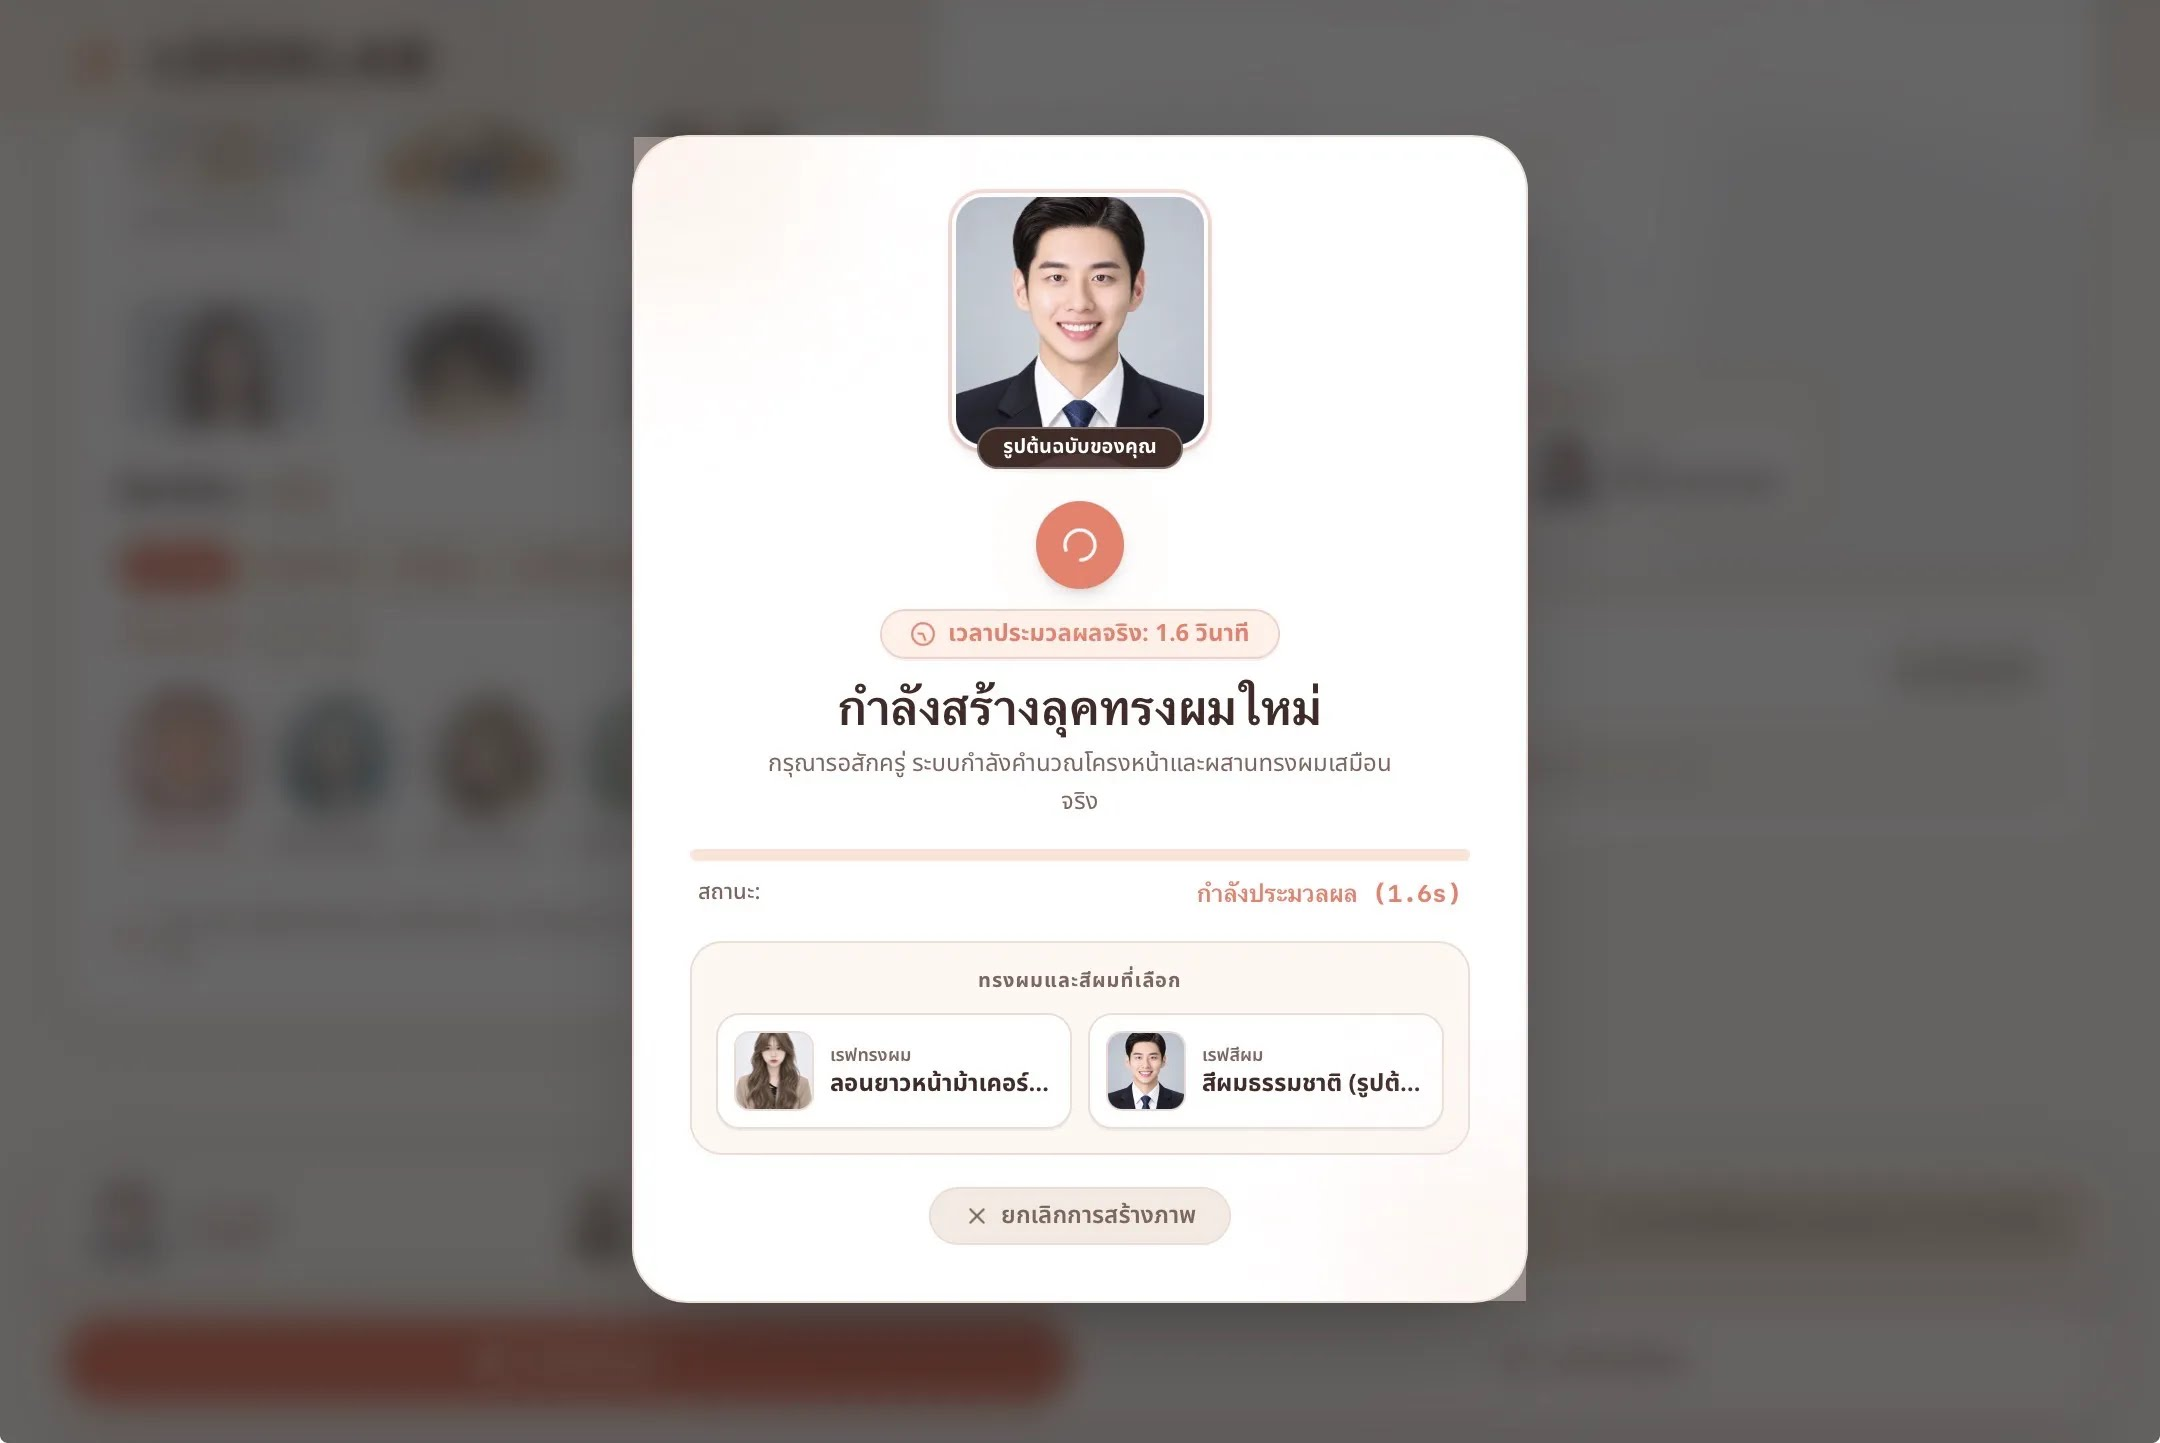
\includegraphics[width=0.8\textwidth]{images/5.jpeg}
\caption{หน้าต่างแสดงสถานะระหว่างสร้างภาพทรงผม}
\label{fig:5}
\end{figure}

\textbf{ขั้นที่ 6 ดูและบันทึกผลลัพธ์}
เมื่อประมวลผลเสร็จ ภาพจะแสดงในโหมด ``สไลด์'' ซึ่งมีแถบเลื่อนแบ่งภาพ
ด้านซ้ายเป็นรูปก่อนเปลี่ยน ด้านขวาเป็นภาพผลลัพธ์
ผู้ใช้ลากปุ่มกลางแถบไปทางซ้ายหรือขวาเพื่อเปรียบเทียบ
หรือกด ``ผลลัพธ์'' เพื่อดูภาพหลังเปลี่ยนทั้งภาพ ดังภาพที่~\ref{fig:7}
ใต้ภาพผลลัพธ์มีส่วน ``ลายน้ำภาพ LOOKLAB'' ให้เลือกเปิดหรือปิดลายน้ำ ซึ่งแสดงที่มุมขวาล่างของภาพ
แล้วกด ``บันทึกภาพผลลัพธ์'' เพื่อเก็บภาพลงเครื่อง
ถ้าต้องการลองทรงผมหรือสีผมอื่นกับรูปเดิม ให้เลือกใหม่แล้วกด ``สร้างลุคใหม่ของคุณ'' อีกครั้งโดยไม่ต้องอัปโหลดรูปใหม่
และถ้าต้องการใช้รูปอื่น ให้กด ``เปลี่ยนรูป'' ที่การ์ด ``รูปภาพของคุณ'' ด้านซ้ายบน

\begin{figure}[!htbp]
\centering
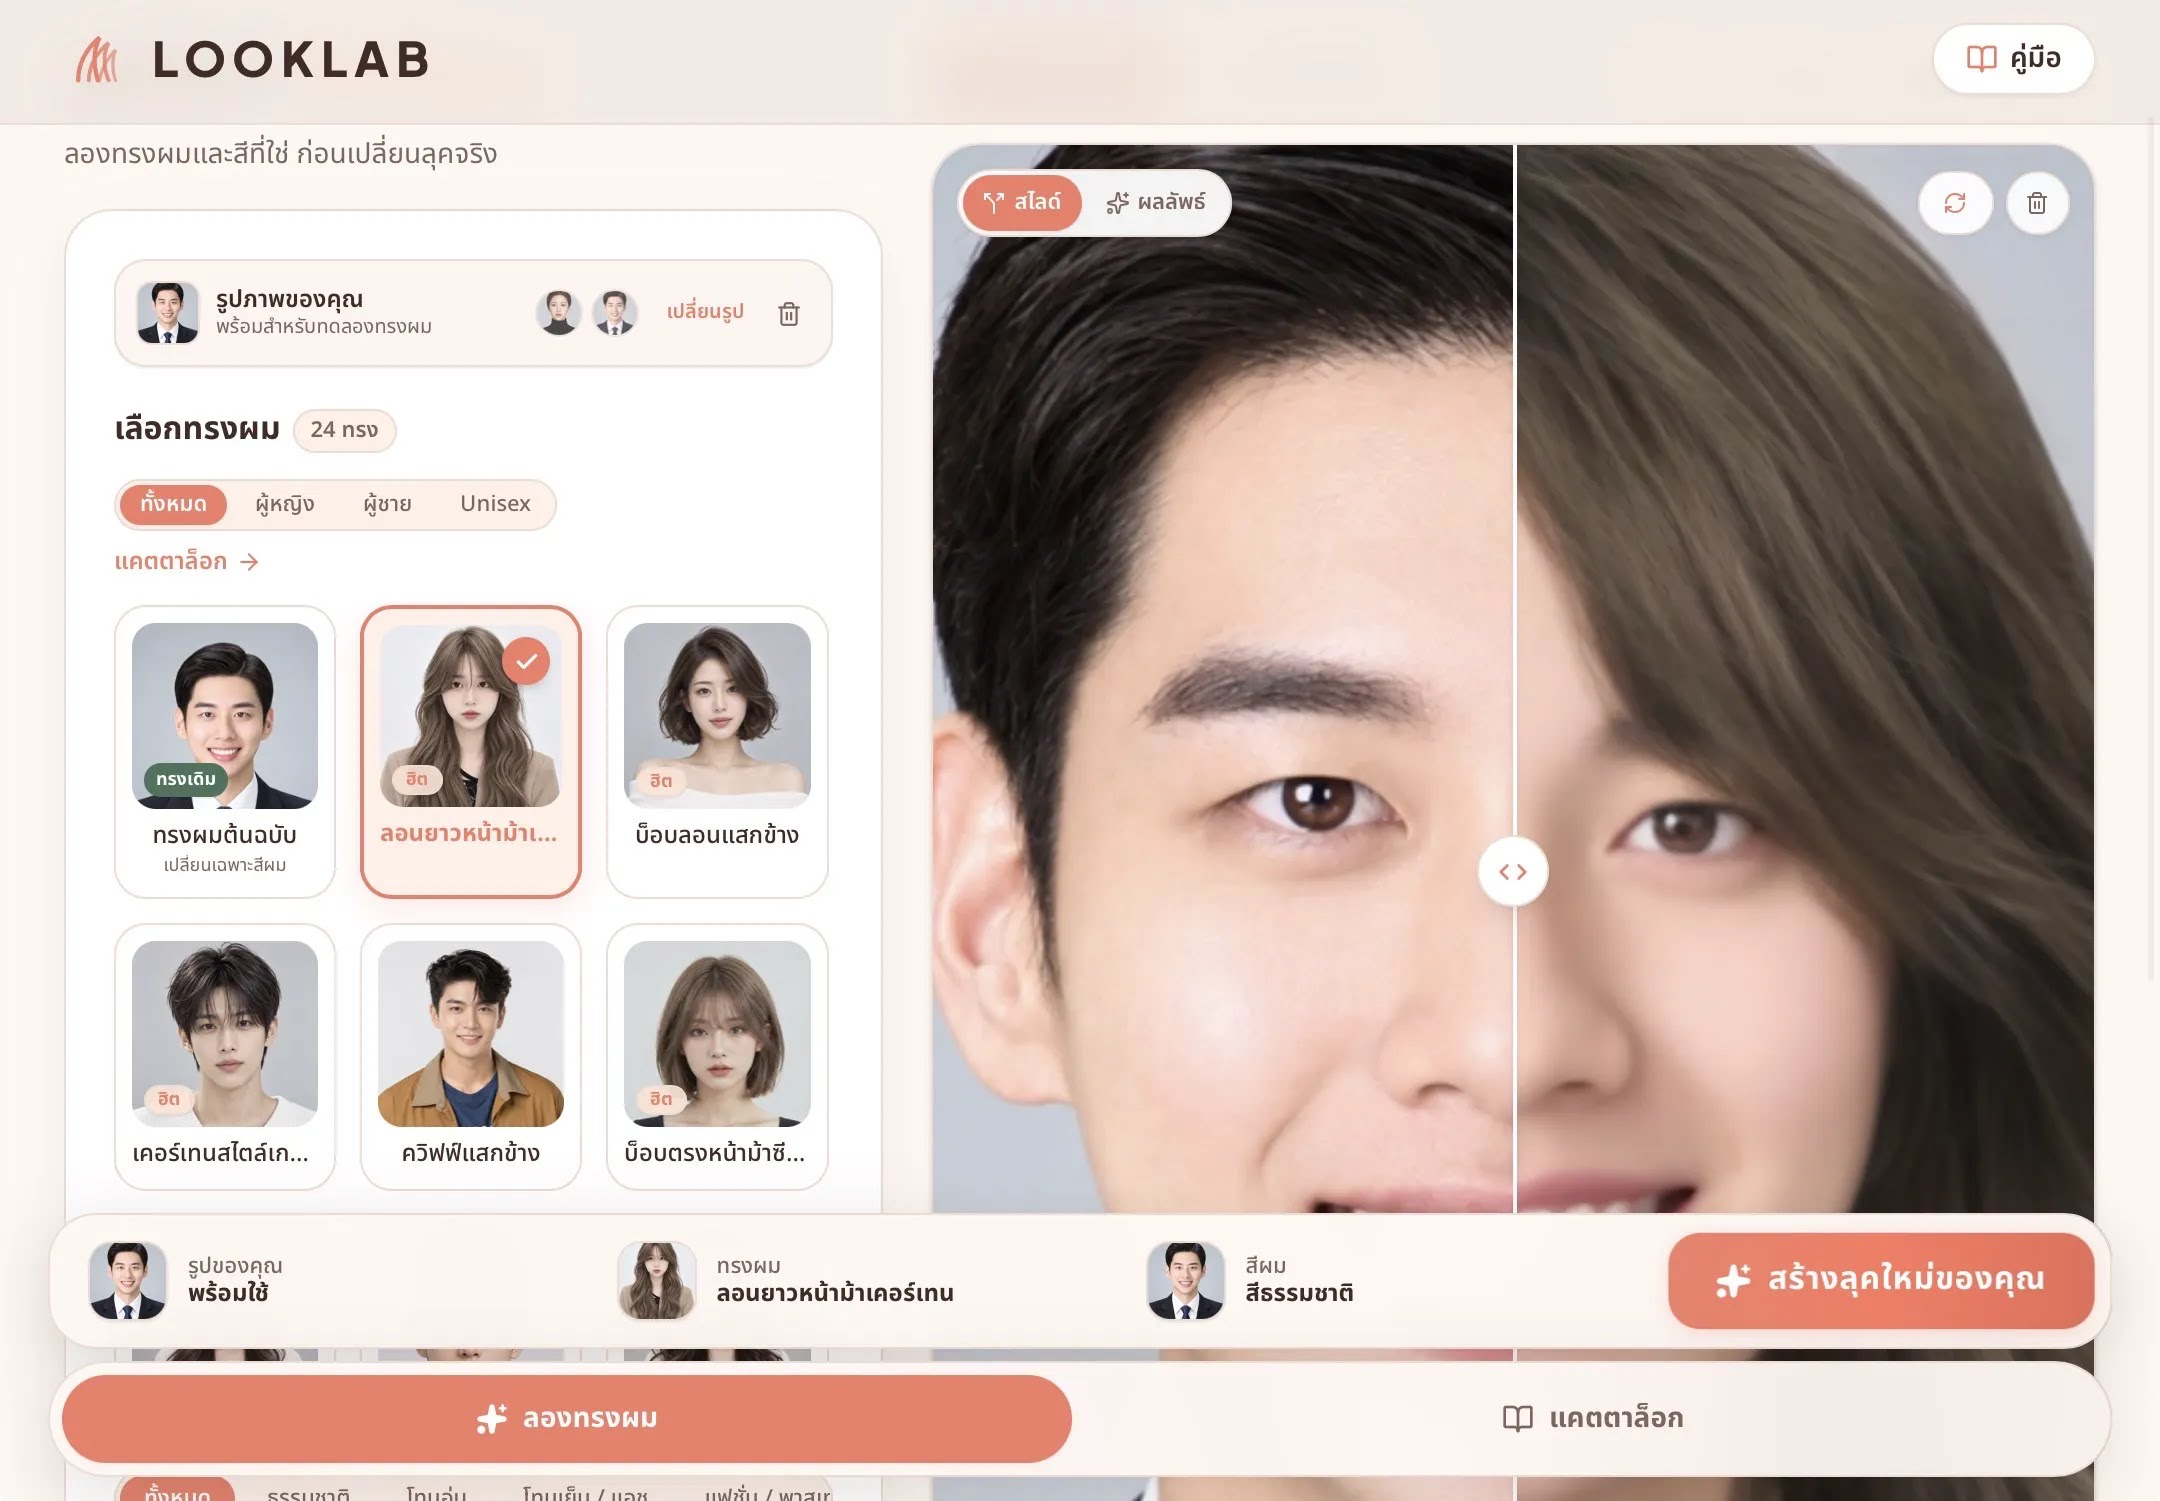
\includegraphics[width=0.9\textwidth]{images/7.jpeg}
\caption{ภาพผลลัพธ์พร้อมแถบเลื่อนเปรียบเทียบก่อนและหลัง}
\label{fig:7}
\end{figure}

\textbf{ขั้นที่ 7 ประเมินผลลัพธ์}
กด ``แบบสอบถามประเมินผลลัพธ์'' เพื่อเปิดหน้าต่างประเมินผลลัพธ์ภาพทรงผม
ด้านบนแสดงเวลารอผลลัพธ์ และภาพเปรียบเทียบ 4 ภาพ คือ รูปต้นฉบับ ภาพอ้างอิงทรงผม ภาพอ้างอิงสีผม และภาพผลลัพธ์
ผู้ใช้คลิกที่ภาพผลลัพธ์หรือกด ``ขยายเต็ม'' เพื่อดูภาพขนาดใหญ่ได้
จากนั้นเลือกช่วงอายุ และให้คะแนนแต่ละข้อเป็นดาว 1 ถึง 5 ดวง
เช่น ทรงผมในภาพผลลัพธ์ตรงตามภาพอ้างอิงทรงผมมากน้อยเพียงใด
ข้อที่มีเครื่องหมายดอกจัน (*) จำเป็นต้องตอบ เมื่อตอบครบแล้วให้ส่งแบบสอบถามที่ท้ายหน้าต่าง
หรือกดปุ่มกากบาทที่มุมขวาบนเพื่อปิดหน้าต่าง
หน้าต่างแบบสอบถามนี้ใช้ร่วมกันทั้งสองโหมด ตัวอย่างหน้าต่างแสดงไว้ในภาพที่~\ref{fig:camera4}

\section{การใช้โหมดกล้องสด}
\label{sec:camera}

โหมดกล้องสดแสดงทรงผมใหม่บนภาพจากกล้อง และให้ทรงผมขยับตามใบหน้า เหมาะกับการดูภาพรวมจากหลายมุม
แต่หลังถ่ายภาพยังต้องรอประมวลผลประมาณ 15 วินาทีก่อนทรงผมใหม่จะปรากฏ
โหมดนี้มี 5 ขั้นตอน ดังนี้

\textbf{ขั้นที่ 1 เปิดกล้อง}
กดปุ่ม ``เปิดกล้อง'' ด้านบนพื้นที่แสดงภาพ ดังภาพที่~\ref{fig:camera1}
เมื่อเบราว์เซอร์ถามสิทธิ์ ให้กดอนุญาตให้เว็บใช้กล้อง
ภาพจากกล้องจะแสดงในพื้นที่ด้านขวา และปุ่มด้านบนจะเปลี่ยนเป็น ``ปิดกล้อง''

\begin{figure}[!htbp]
\centering
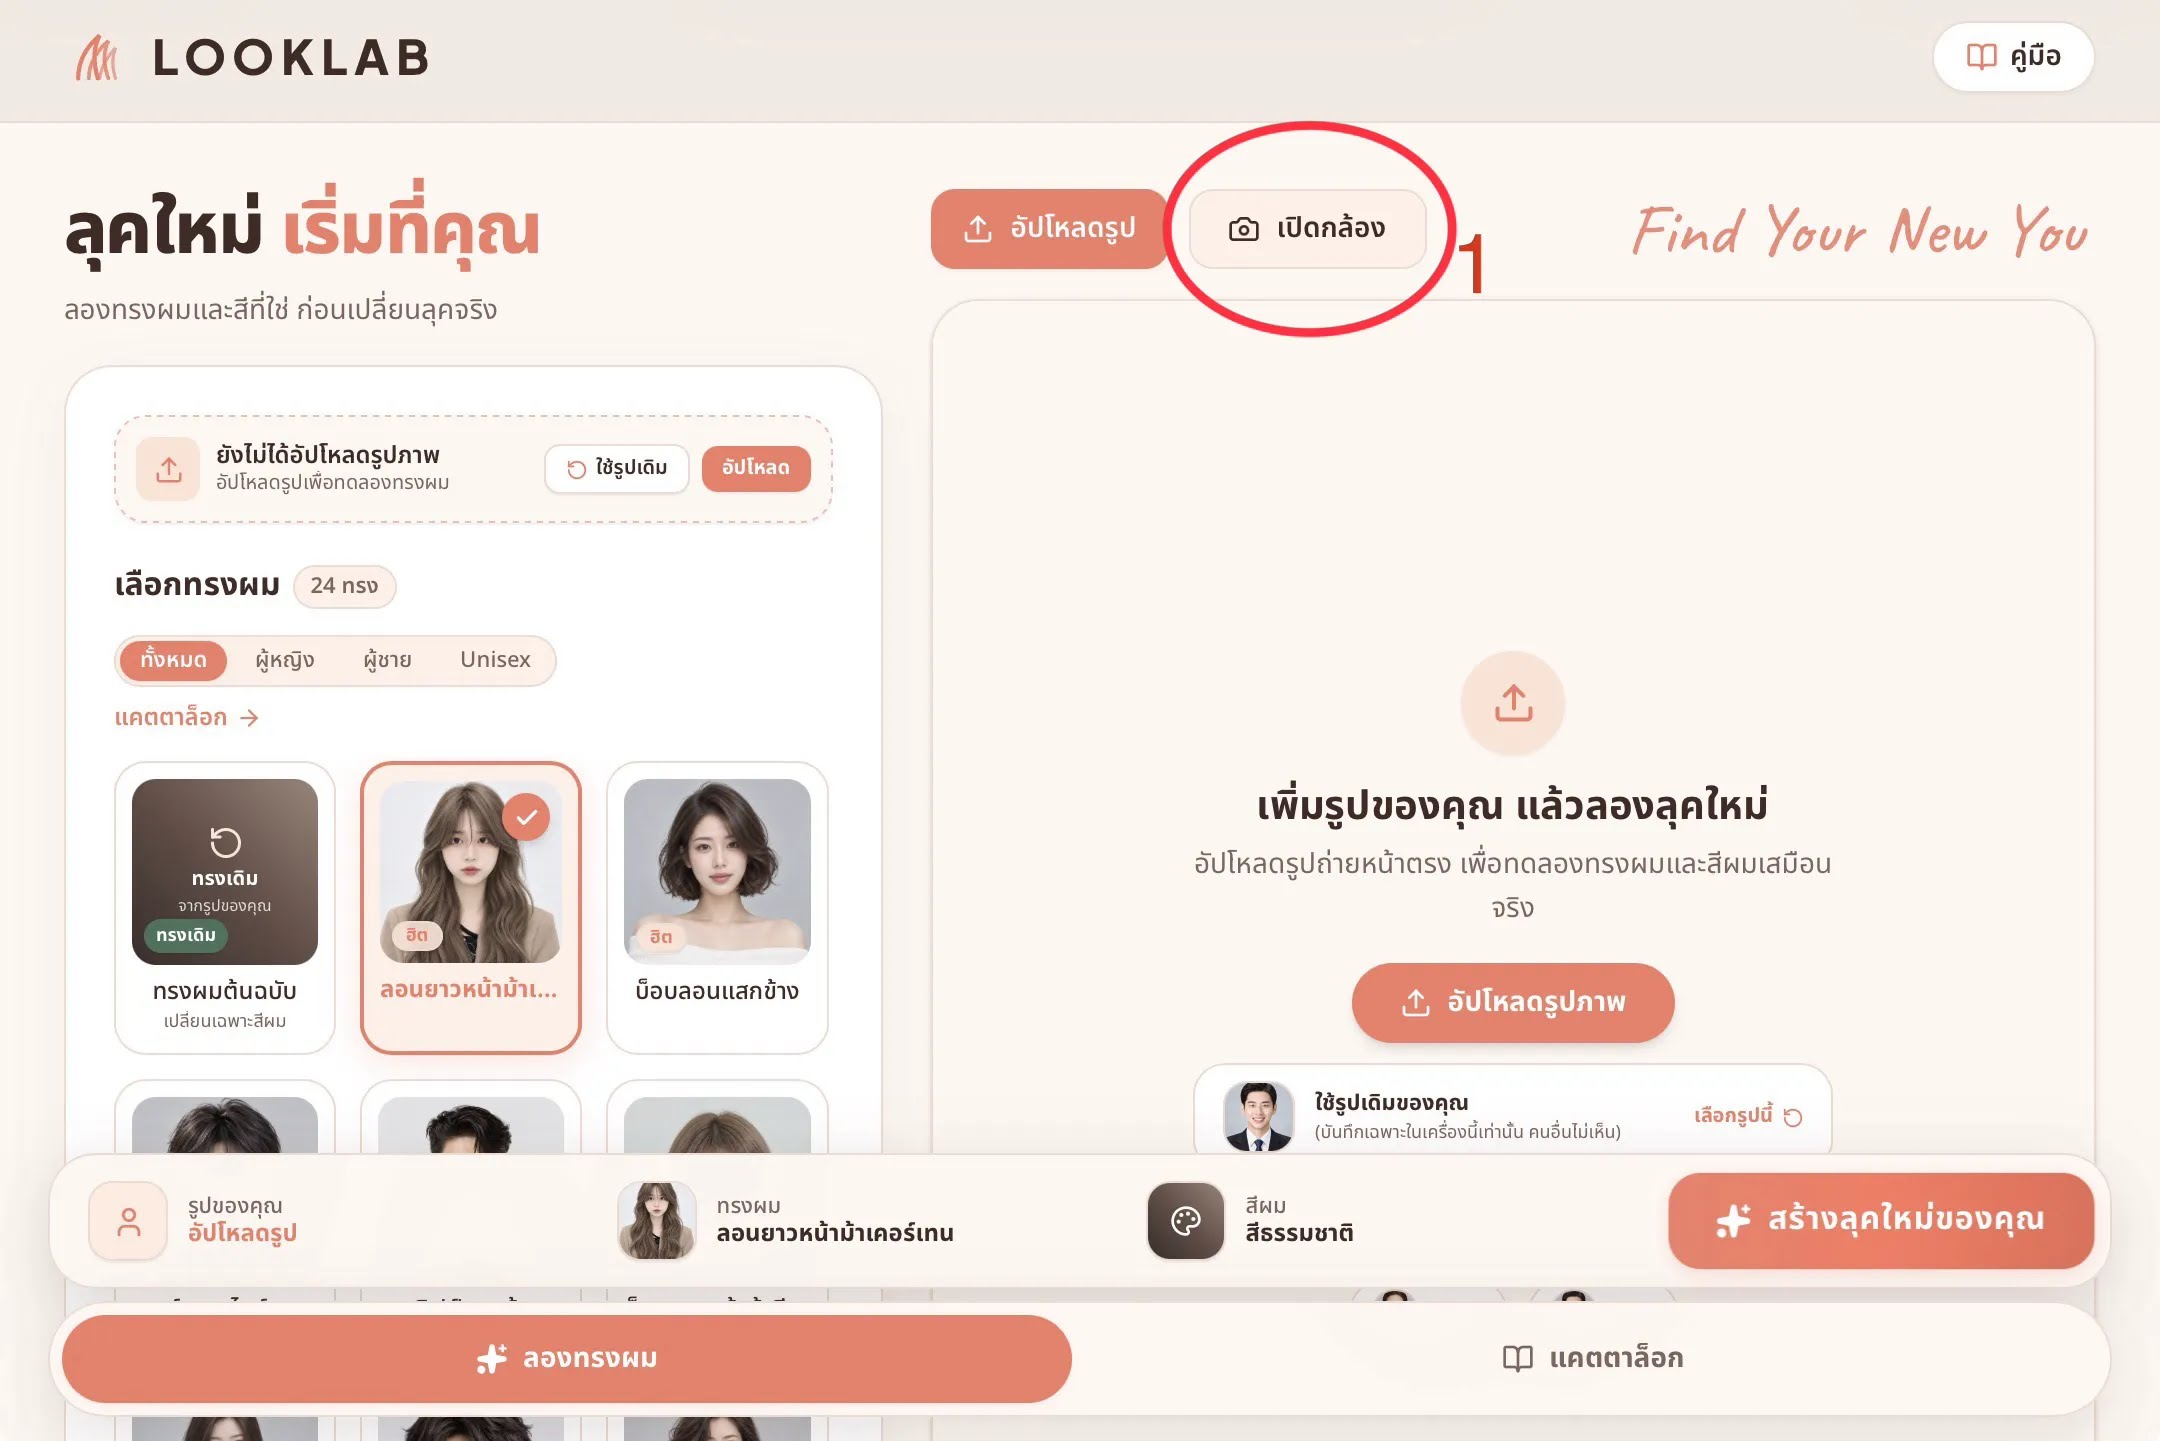
\includegraphics[width=0.9\textwidth]{images/camera1.jpeg}
\caption{ปุ่มเปิดกล้องสำหรับเข้าสู่โหมดกล้องสด}
\label{fig:camera1}
\end{figure}

\textbf{ขั้นที่ 2 เลือกทรงผม}
เลือกทรงผมจากแผงด้านซ้ายเหมือนโหมดอัปโหลดรูป
ในโหมดนี้การ์ด ``ทรงผมต้นฉบับ'' หมายถึงทรงผมจริงจากกล้องสด
และช่องแรกของแถบด้านล่างจะแสดงเป็น ``กล้องของคุณ'' พร้อมสถานะ ``กล้องสดเรียลไทม์''
ทรงที่เลือกจะแสดงในช่อง ``ทรงผม'' ของแถบด้านล่าง

\textbf{ขั้นที่ 3 เลือกสีผมและถ่ายภาพ}
เลือกสีผมจากส่วน ``เลือกสีผม'' ในแผงด้านซ้ายเหมือนโหมดอัปโหลดรูป
ชื่อสีที่เลือกจะแสดงในช่อง ``สีผม'' ของแถบด้านล่าง
จากนั้นหันหน้าตรงเข้าหากล้องในระยะที่เห็นตั้งแต่ศีรษะถึงหัวไหล่ ระบบจะบอกให้ขยับใบหน้าจนอยู่ในวงรี
เมื่ออยู่ในตำแหน่งแล้ว วงรีจะเปลี่ยนเป็นสีฟ้าและนับถอยหลัง 5 วินาที
โดยมุมซ้ายบนของภาพจะแสดงเวลาที่เหลือก่อนถ่ายภาพ ให้อยู่นิ่งจนถ่ายภาพเสร็จ
ภาพที่~\ref{fig:camera2-3} แสดงช่องทรงผม (ขั้นที่ 2) และช่องสีผม (ขั้นที่ 3) ในแถบด้านล่าง
ระหว่างที่ระบบกำลังนับถอยหลังเพื่อถ่ายภาพ

\begin{figure}[H]
\centering
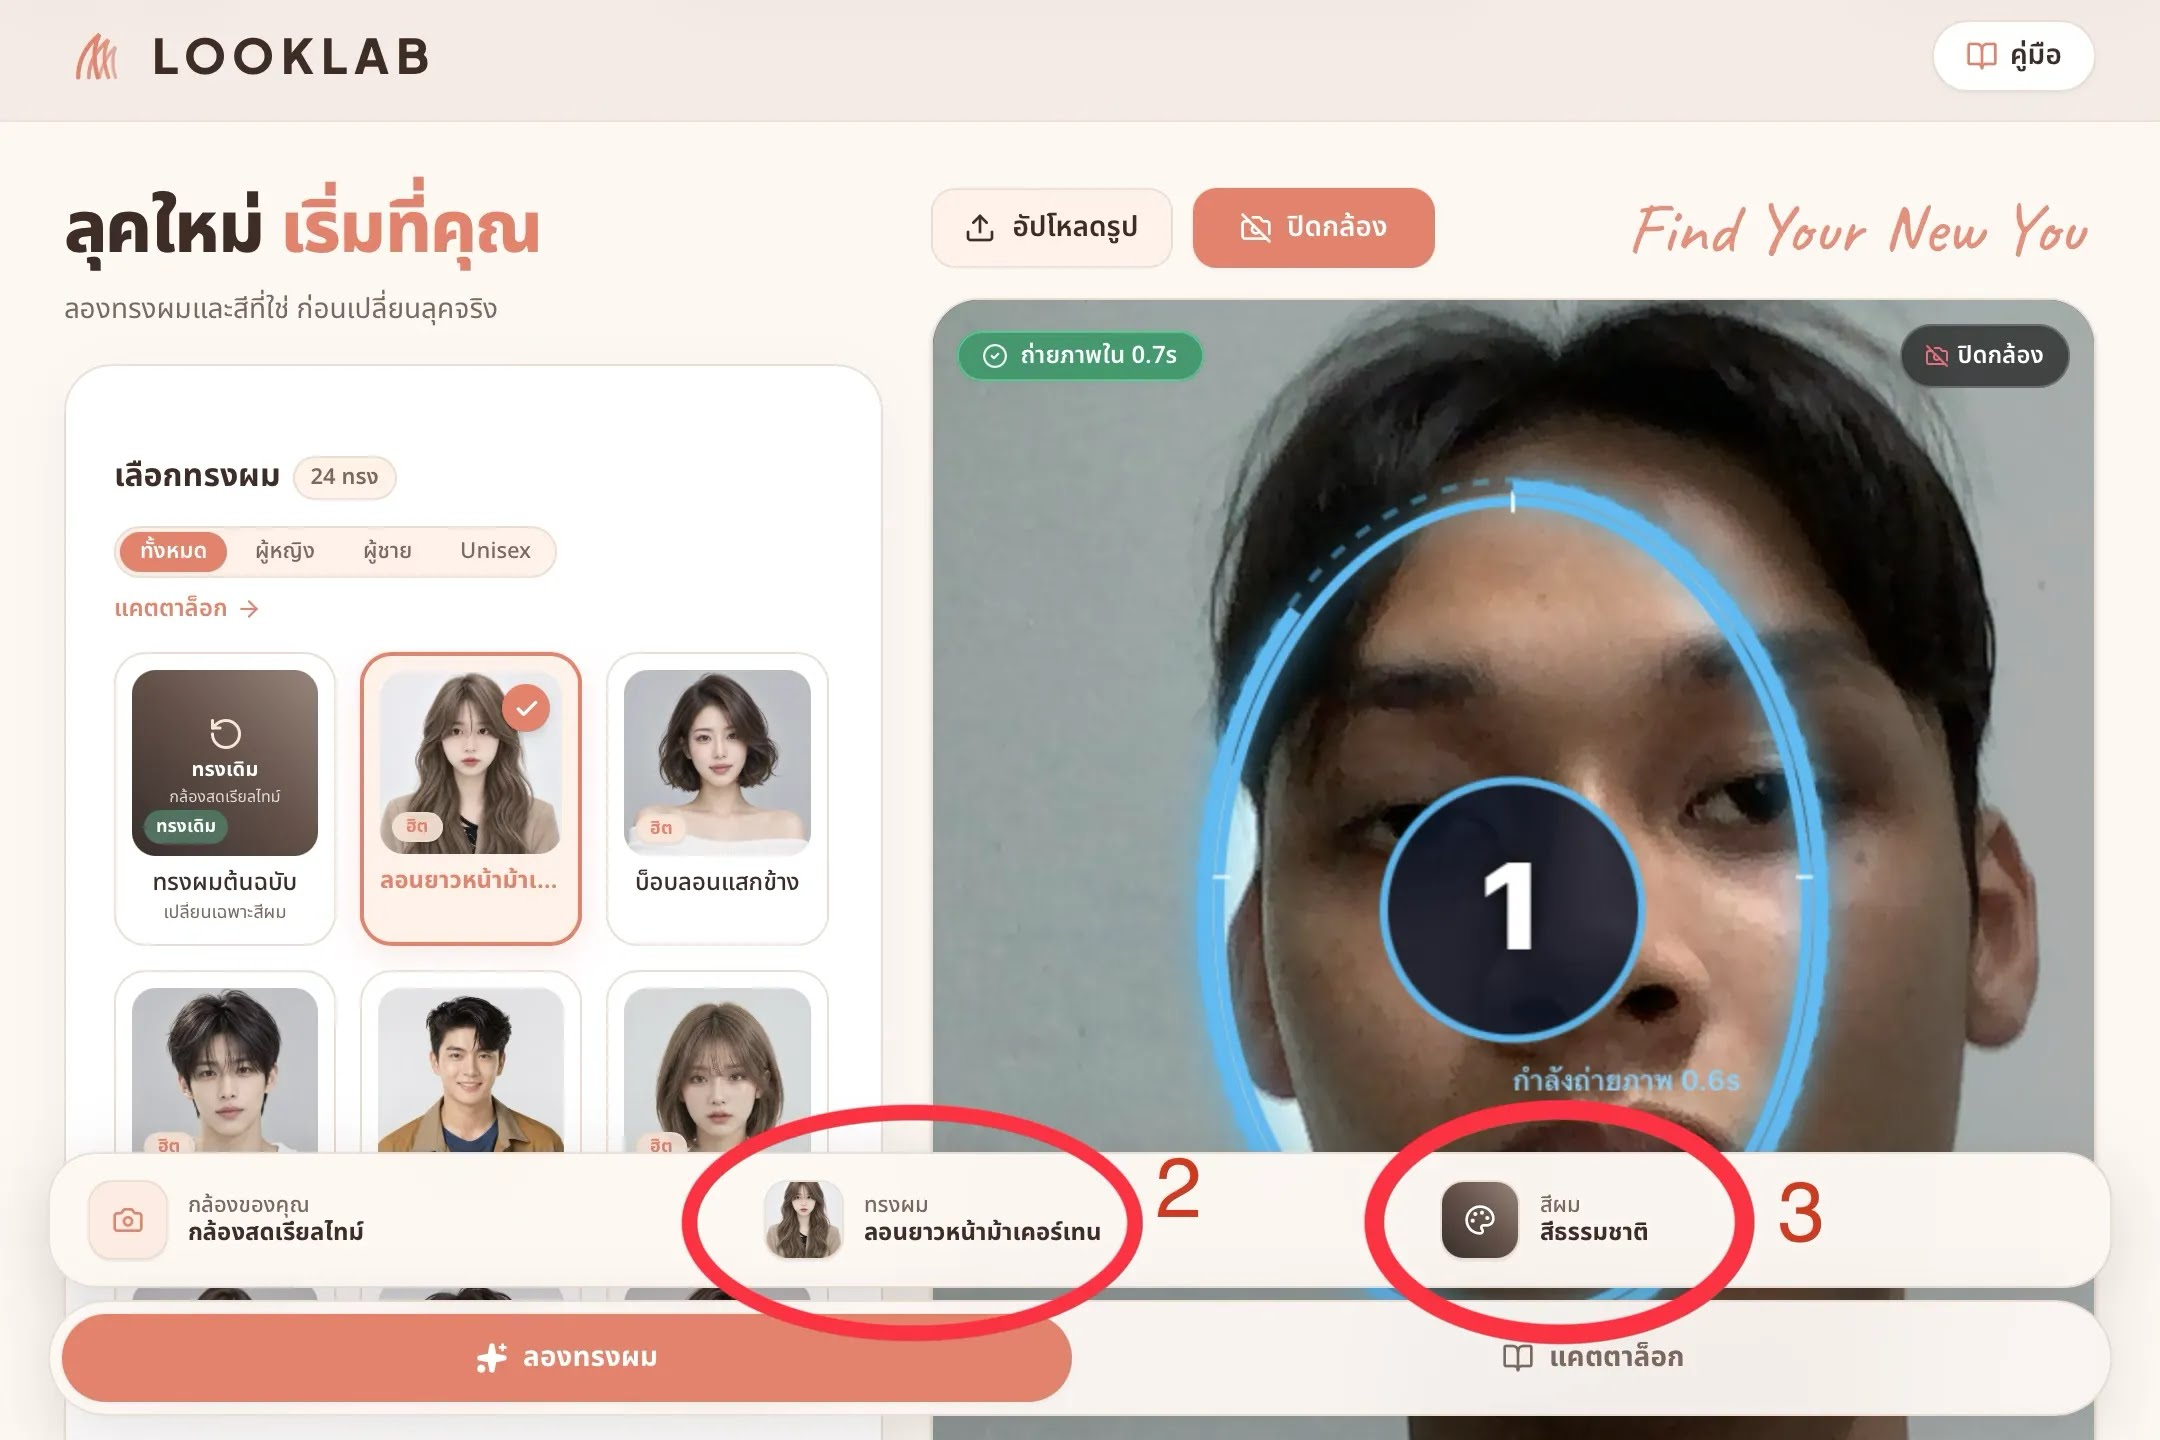
\includegraphics[width=0.9\textwidth]{images/camera2-3.jpeg}
\caption{การเลือกทรงผม สีผม และการนับถอยหลังเพื่อถ่ายภาพในโหมดกล้องสด}
\label{fig:camera2-3}
\end{figure}

\textbf{ขั้นที่ 4 ประเมินผลลัพธ์}
หลังถ่ายภาพเสร็จ ระบบจะนำภาพที่ถ่ายจากกล้องไปสร้างภาพผลลัพธ์ตามทรงผมและสีผมที่เลือก
ผู้ใช้ประเมินผลลัพธ์ได้ด้วยแบบสอบถามเดียวกับขั้นที่ 7 ของโหมดอัปโหลดรูป
ซึ่งแสดงรูปที่ถ่ายจากกล้อง ภาพอ้างอิงทรงผม ภาพอ้างอิงสีผม และภาพผลลัพธ์เทียบกัน ดังภาพที่~\ref{fig:camera4}

\begin{figure}[!htbp]
\centering
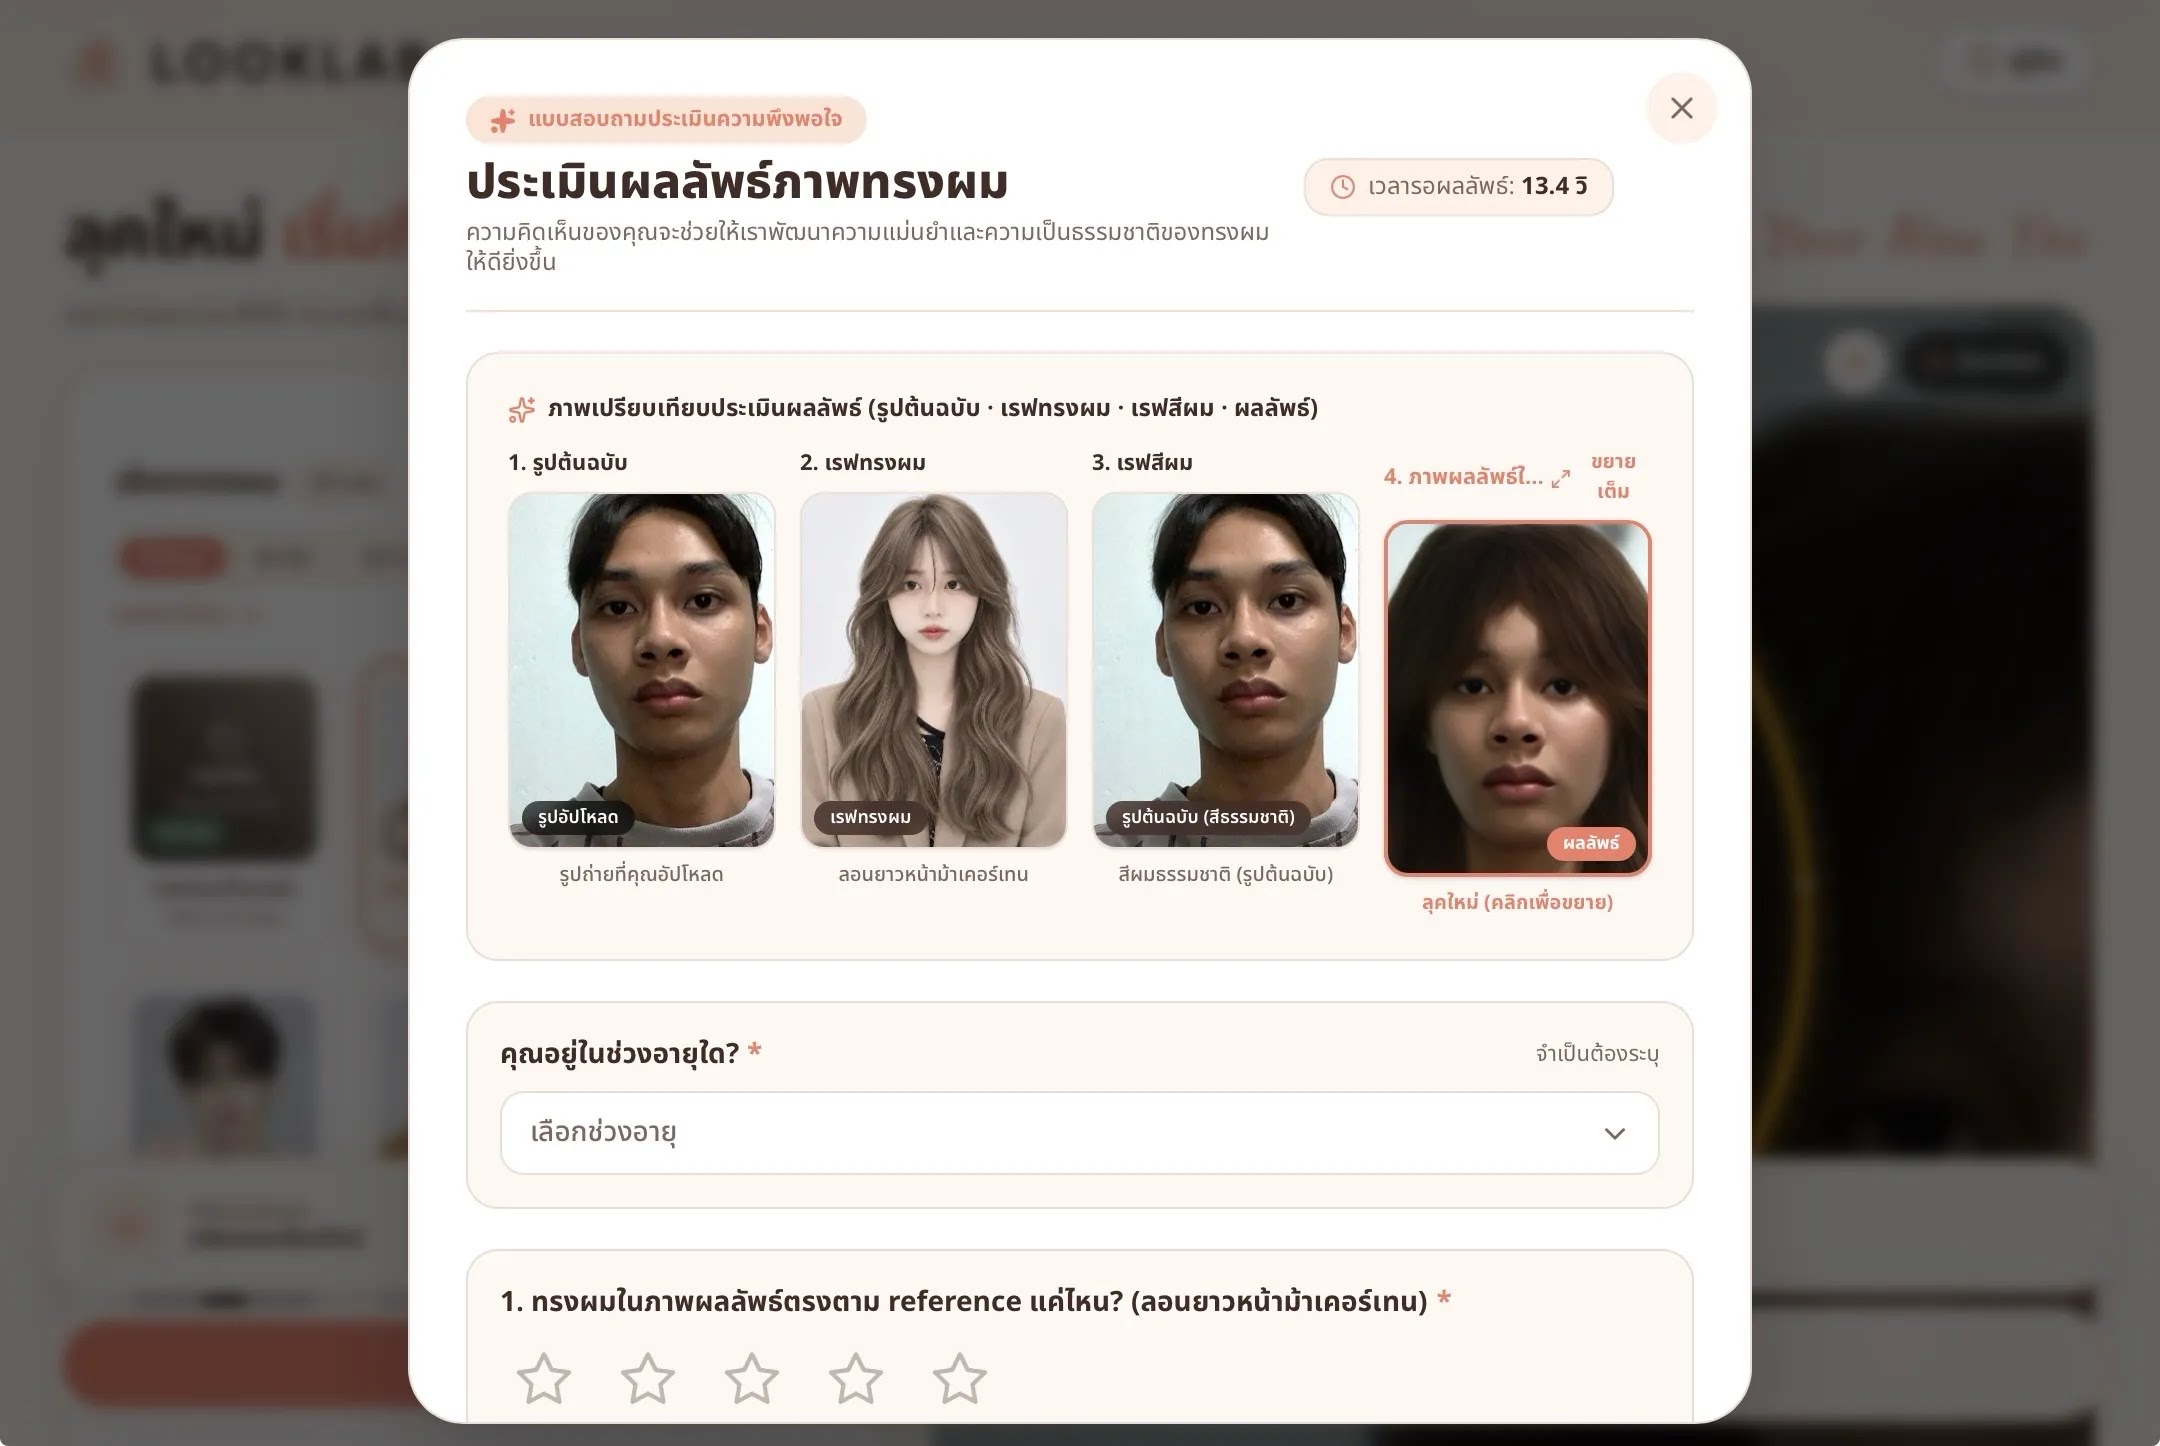
\includegraphics[width=0.8\textwidth]{images/camera4.jpeg}
\caption{หน้าต่างแบบสอบถามประเมินผลลัพธ์ภาพทรงผมจากภาพที่ถ่ายด้วยกล้อง}
\label{fig:camera4}
\end{figure}

\textbf{ขั้นที่ 5 ดูทรงผมบนกล้องสดและบันทึกภาพ}
ทรงผมใหม่จะปรากฏบนภาพจากกล้องและขยับตามศีรษะ ดังภาพที่~\ref{fig:camera5}
ถ้าใบหน้าเลื่อนออกจากกลางกรอบ วงรีจะเปลี่ยนเป็นสีส้มพร้อมข้อความ ``ขยับใบหน้าให้อยู่ตรงกลางกรอบ''
ให้ขยับใบหน้ากลับเข้ากลางกรอบเพื่อให้ทรงผมวางได้ตรงตำแหน่ง
ผู้ใช้กด ``บันทึกภาพนิ่ง'' ที่มุมขวาล่างเพื่อเก็บภาพ และกด ``ปิดกล้อง'' เมื่อใช้งานเสร็จ
ถ้าต้องการภาพคุณภาพสูงที่สุด แนะนำให้ใช้โหมดอัปโหลดรูป

\begin{figure}[!htbp]
\centering
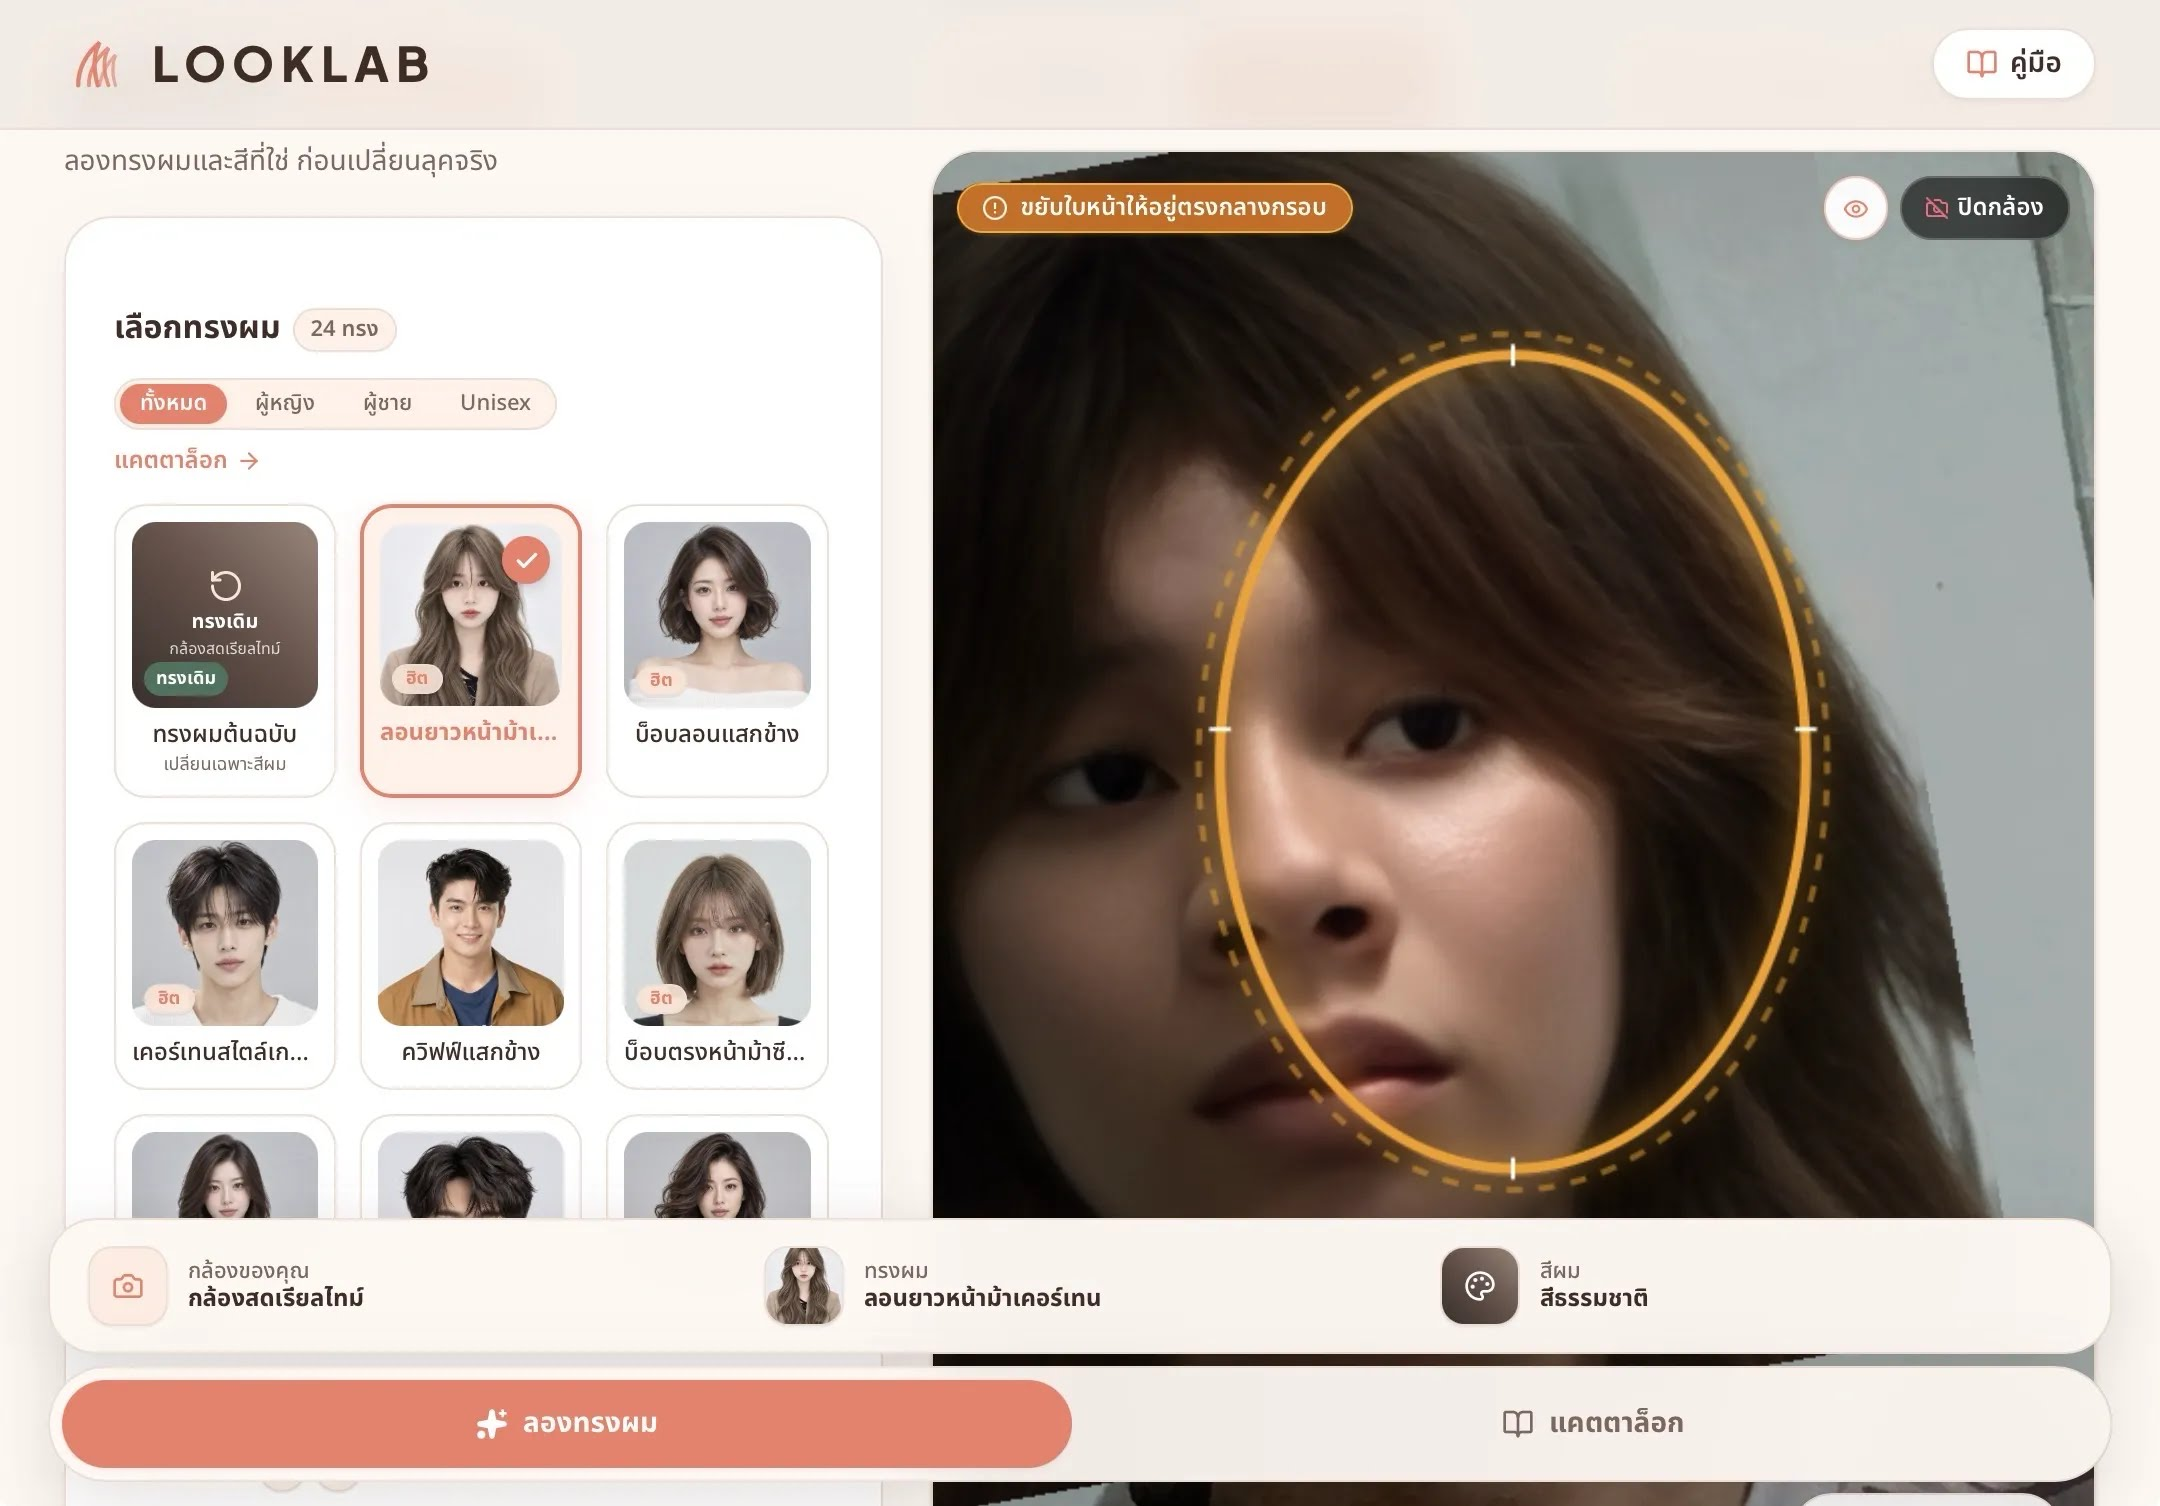
\includegraphics[width=0.9\textwidth]{images/camera5.jpeg}
\caption{ทรงผมใหม่ที่แสดงบนภาพจากกล้องแบบเรียลไทม์}
\label{fig:camera5}
\end{figure}

\section{ข้อแนะนำในการเตรียมรูป}
\label{sec:photo_tips}

ระบบทำงานได้ดีที่สุดกับรูปหน้าตรงในระดับสายตา ที่มีแสงสว่างสม่ำเสมอจากด้านหน้าและไม่ย้อนแสง
ควรรวบผมหรือทัดผมให้เห็นหน้าผากและใบหู เพราะผมเดิมที่ปรกหน้าอาจโผล่ทับทรงผมใหม่
ควรถอดแว่นกรอบหนา หมวก หรือที่คาดผม ทำสีหน้าปกติ และไม่เอียงศีรษะ
ฉากหลังควรเรียบและไม่กลืนกับสีผม และควรใช้รูปที่คมชัดและไม่ผ่านฟิลเตอร์ปรับรูปหน้า
ข้อแนะนำนี้ใช้กับการถ่ายภาพในโหมดกล้องสดด้วย

\section{การแก้ปัญหาเบื้องต้น}

ถ้าระบบเตือนว่าไม่พบใบหน้า หรือวางทรงผมผิดตำแหน่ง ส่วนใหญ่เกิดจากรูปมืด ย้อนแสง หรือหน้าเอียง
ให้ถ่ายรูปใหม่ตามข้อแนะนำในหัวข้อที่~\ref{sec:photo_tips} แล้วลองอีกครั้ง

ถ้าเปิดกล้องไม่ได้ ให้ตรวจสอบว่าได้อนุญาตให้เว็บใช้กล้องในการตั้งค่าของเบราว์เซอร์แล้ว
และไม่มีโปรแกรมอื่นใช้กล้องอยู่ จากนั้นรีเฟรชหน้าเว็บแล้วกด ``เปิดกล้อง'' อีกครั้ง

ถ้าการสร้างภาพใช้เวลานานกว่าปกติมาก ให้ตรวจสอบการเชื่อมต่ออินเทอร์เน็ต
แล้วกด ``ยกเลิกการสร้างภาพ'' และกด ``สร้างลุคใหม่ของคุณ'' อีกครั้ง

ถ้ามีข้อสงสัยอื่น ผู้ใช้เปิดแท็บคำถามที่พบบ่อยในหน้าต่างคู่มือได้จากปุ่ม ``คู่มือ'' ที่มุมขวาบน

% =============================
% ภาคผนวก จ
% =============================
\appendiceschapter{การนำ Artificial Intelligence (AI) มาใช้ในงานวิจัย}
\label{app:ai}

\renewcommand{\thesection}{จ.\arabic{section}}
\setcounter{section}{0}

ภาคผนวกนี้บันทึกว่าผู้วิจัยใช้ AI ในขั้นไหนของโครงงานบ้าง โดย AI ที่ใช้ในหัวข้อที่ จ.1 ถึง จ.9 คือ ChatGPT หัวข้อที่ จ.10 คือ Google AI Studio และหัวข้อที่ จ.11 คือ Claude
แต่ละหัวข้อเริ่มจากข้อความสั่งงาน (Prompt) ที่ผู้วิจัยพิมพ์จริง ตามด้วยสรุปว่า AI ตอบอะไรกลับมา
และปิดท้ายด้วยสิ่งที่ผู้วิจัยทำกับคำตอบนั้น คือนำไปใช้เลย นำไปปรับก่อนใช้ หรือนำไปตรวจสอบกับงานวิจัย โค้ด และผลการรันจริงก่อน
หลักที่ผู้วิจัยยึดตลอดคือคำตอบของ AI เป็นเพียงจุดเริ่มต้น ไม่ใช่ข้อเท็จจริงที่เชื่อได้ทันที
ทุกค่าที่รายงานในบทที่ 3 และบทที่ 4 มาจากโค้ดที่ผู้วิจัยรันเองและผลที่วัดได้จริง ไม่ได้มาจากคำตอบของ AI

\section{การสร้าง Colab ทดลอง HairFastGAN แบบ Pretrained \mbox{(ChatGPT)}}
\label{sec:ai_colab}

ขั้นแรกของโครงงาน ผู้วิจัยต้องการรัน HairFastGAN ด้วยน้ำหนักที่ผู้พัฒนาฝึกไว้แล้ว (Pretrained)
เพื่อดูว่าโมเดลตั้งต้นให้ผลอย่างไร จึงแนบไฟล์งานวิจัย HairFastGAN (arXiv:2404.01094v3) ให้ ChatGPT และส่งข้อความดังนี้
\begin{quote}
\small ``ช่วยอ่านงานวิจัยที่แนบกับโค้ดใน \url{https://github.com/AIRI-Institute/HairFastGAN}
แล้วทำไฟล์ Colab ให้ผมหน่อย ขอให้ติดตั้งและโหลดโมเดลมา pretrained ได้
อัปโหลดรูปหน้า รูปทรงผม และรูปสีผมเพื่อสร้างภาพผลลัพธ์ได้ สามารถใช้งานได้ทั้งแต่ต้นจนจบ
พร้อมอธิบายและสรุปให้ผมเข้าใจด้วย''
\end{quote}

ChatGPT ตอบกลับเป็นไฟล์ \texttt{HairFastGAN\_Pretrained\_\allowbreak Thai\_Colab.ipynb} พร้อมคำอธิบายภาษาไทย ดังภาพที่~\ref{fig:ai_colab}
ในไฟล์มีขั้นตอนครบตั้งแต่ตรวจ GPU ติดตั้ง Python 3.10 กับ PyTorch 1.13.1 ตามที่โครงการเดิมใช้
ดาวน์โหลดน้ำหนักจาก Hugging Face โดยล็อกรุ่นของโค้ดและน้ำหนักไว้ อัปโหลดภาพทีละบทบาท
แล้วเรียก \texttt{HairFast.swap(..., align=True)} ของโครงการเพื่อสร้างภาพขนาด $1024 \times 1024$
และอธิบายลำดับโมดูล Embedding, Pose, Shape, Color และ Refinement ตามงานวิจัย
AI ระบุไว้เองด้วยว่าตรวจเพียงโครงสร้างไฟล์และไวยากรณ์ของโค้ด ยังไม่ได้รันจริงบน GPU
และได้เปลี่ยนตัวดำเนินการของ StyleGAN2 เป็นแบบ PyTorch ล้วนเพื่อเลี่ยงการคอมไพล์ CUDA
ซึ่งอาจทำให้ความเร็วและตัวเลขต่างจากต้นฉบับเล็กน้อย

\begin{figure}[H]
\centering
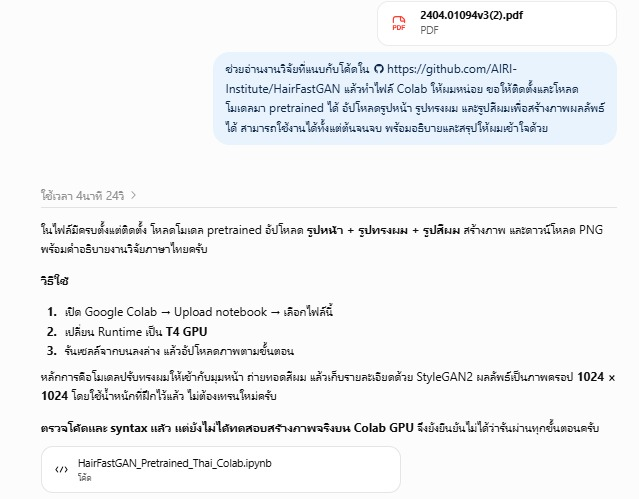
\includegraphics[width=0.6\textwidth]{images/ai_prompt_colab.jpg}
\caption{ข้อความสั่งงานและคำตอบของ ChatGPT ในการสร้าง Colab สำหรับรัน HairFastGAN แบบ Pretrained}
\label{fig:ai_colab}
\par\vspace{3pt}{\footnotesize\raggedright หมายเหตุ: AI = Artificial Intelligence (ปัญญาประดิษฐ์), GPU = Graphics Processing Unit (หน่วยประมวลผลกราฟิก), T4 = รุ่นของ GPU ที่ Colab มีให้ใช้\par}
\end{figure}

ผู้วิจัยไม่ได้ใช้ไฟล์นี้ตามที่ได้มาทั้งหมด แต่ใช้เป็นจุดเริ่มต้นในการทำความเข้าใจโค้ดและรันโมเดลตั้งต้น
สิ่งที่ผู้วิจัยตรวจก่อนคือคำอธิบายโมดูลทั้งห้า ว่าตรงกับงานวิจัยและไฟล์ \texttt{hair\_swap.py}
และ \texttt{models/} ใน GitHub หรือไม่ ซึ่งเป็นพื้นฐานของหัวข้อที่~\ref{sec:hairfastgan}
จากนั้นนำโค้ดไปรันจริงบน Colab และแก้ปัญหาที่เกิดระหว่างติดตั้ง
เมื่อเข้าสู่ขั้นทดลองจริง ผู้วิจัยย้ายไปใช้ GPU A100 และเขียนสมุดบันทึกของตัวเองเพิ่ม
ให้โหลดน้ำหนักที่ปรับจูนแล้วพร้อมตรวจค่าแฮชของไฟล์
ตั้งค่าการผสม $F$ เป็น 0.95 และปิดการหมุนภาพทรงผมให้เหมือนกันทั้งตอนฝึกและตอนทดสอบ
รวมทั้งเก็บเวลาประมวลผลของแต่ละขั้นแยกกัน
ส่วนเวลาที่ได้จาก Colab ฉบับนี้ ผู้วิจัยไม่ได้นำไปรายงาน เพราะใช้ตัวดำเนินการคนละแบบกับต้นฉบับ ตามที่ AI เตือนไว้

\section{การเพิ่มขั้นปรับภาพด้วย Realistic Vision V5.1 \mbox{(ChatGPT)}}
\label{sec:ai_diffusion}

หลังได้ภาพจาก HairFastGAN แล้ว ผู้วิจัยเห็นว่าเส้นผมยังนุ่มและเบลอ จึงขอให้ ChatGPT เพิ่มขั้นปรับภาพต่อท้าย
\begin{quote}
\small ``จากโค้ดเดิม ช่วยเพิ่มขั้นตอนปรับภาพด้วย Stable Diffusion โมเดล Realistic Vision V5.1
ต่อจากภาพผลลัพธ์ให้หน่อย อยากให้หน้าและเส้นผมดูคมชัดเป็นธรรมชาติมากขึ้น
โดยรักษาหน้าตา ทรงผม และสีผมจากภาพเดิมให้มากที่สุด แสดงภาพก่อนและหลังพร้อมเวลาประมวลผล
และบันทึกรูปได้ ทำเป็นเซลล์เพิ่มใน Colab ให้ด้วย''
\end{quote}

ChatGPT ตอบกลับเป็นเซลล์เพิ่มเติม (\texttt{Realistic\_Vision\_\allowbreak V51\_Addon\_\allowbreak Cells.ipynb}) ดังภาพที่~\ref{fig:ai_diffusion}
แนวทางของ AI คือแปลงทั้งภาพแบบ Image-to-Image ด้วยรุ่น \texttt{Realistic\_Vision\_V5.1\_noVAE}
คู่กับ VAE (Variational Autoencoder) รุ่น \texttt{sd-vae-ft-mse} ตัวลบสัญญาณรบกวน DPM-Solver++
ความแรง 0.18 ค่านำทาง 3.5 จำนวน 30 ขั้น แล้วนำผลมาผสมกลับกับภาพเดิมทั้งภาพที่สัดส่วน 0.65
พร้อมแสดงภาพก่อน ภาพ Diffusion ล้วน และภาพหลังผสม และแยกเวลาโหลดโมเดลออกจากเวลาปรับภาพ
AI เตือนไว้ด้วยว่าข้อความสั่งงานไม่ได้ล็อกใบหน้า และขั้นนี้ไม่รับประกันว่าภาพจะคมขึ้นทุกภาพ

\begin{figure}[H]
\centering
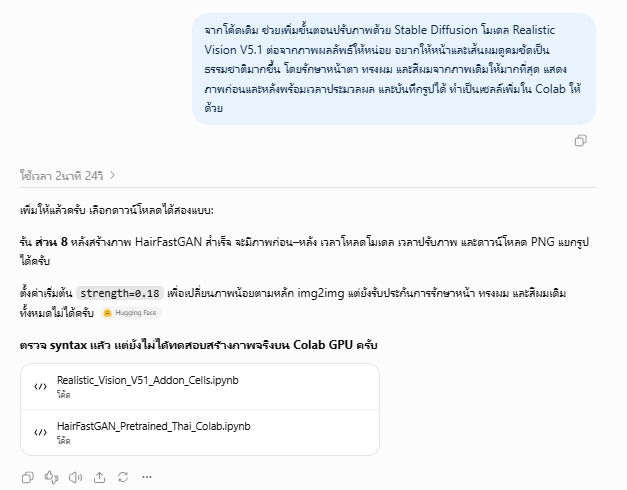
\includegraphics[width=0.6\textwidth]{images/ai_prompt_diffusion.jpg}
\caption{ข้อความสั่งงานและคำตอบของ ChatGPT ในการเพิ่มขั้นปรับภาพด้วย Realistic Vision V5.1}
\label{fig:ai_diffusion}
\par\vspace{3pt}{\footnotesize\raggedright หมายเหตุ: AI = Artificial Intelligence (ปัญญาประดิษฐ์), GPU = Graphics Processing Unit (หน่วยประมวลผลกราฟิก)\par}
\end{figure}

ผู้วิจัยใช้คำตอบนี้เป็นแนวคิดตั้งต้นเท่านั้น และเปลี่ยนวิธีเกือบทั้งหมดก่อนนำไปใช้จริง
เหตุผลหลักคือการแปลงทั้งภาพแบบ Image-to-Image ทำให้พื้นหลังและเสื้อผ้าเปลี่ยนไปด้วย
และการผสมภาพทั้งภาพที่สัดส่วนคงที่ไม่ได้แยกว่าส่วนไหนควรเปลี่ยนมากหรือน้อย
ขั้นที่ใช้จริง (หัวข้อที่~\ref{sec:diffusion}) จึงเปลี่ยนเป็น Stable Diffusion Inpainting
ที่ใช้ SegFormer-B2 สร้างหน้ากากให้แก้ได้เฉพาะผมกับใบหน้า ลดความแรงเหลือ 0.15 ลดค่านำทางเหลือ 2.5
ใช้ตัวลบสัญญาณรบกวน UniPC (Unified Predictor-Corrector) และเขียนข้อความสั่งงานใหม่
จากนั้นเพิ่มขั้นเก็บพื้นหลังและขั้นเพิ่มความคมที่ผู้วิจัยออกแบบเอง
ค่าที่เลือกทั้งหมดมาจากการทดลองเปรียบเทียบของผู้วิจัย เช่น การเทียบข้อความสั่งงาน 6 แบบในภาคผนวก~ค
และวัดผลด้วย MUSIQ (Multi-scale Image Quality Transformer) ArcFace IoU (Intersection over Union) และความเห็นของผู้ใช้ในบทที่ 4
สิ่งที่ผู้วิจัยคงไว้จากคำตอบของ AI มีเพียงแนวคิดใช้ความแรงต่ำ การแสดงภาพก่อนและหลังเทียบกัน
และการแยกเวลาโหลดโมเดลออกจากเวลาประมวลผล

\section{การวิเคราะห์ว่าส่วนไหนของ HairFastGAN ปรับจูนได้ \mbox{(ChatGPT)}}
\label{sec:ai_finetune}

ก่อนเริ่มปรับจูน ผู้วิจัยต้องการรู้ว่าโค้ดของ HairFastGAN เปิดให้ฝึกส่วนไหนได้บ้าง
และต้องการแยกให้ชัดว่าอะไรคือการปรับจูนน้ำหนักจริง อะไรเป็นแค่การปรับค่าตอนสร้างภาพ จึงถาม ChatGPT ว่า
\begin{quote}
\small ``ช่วยดูงานวิจัย โค้ดใน github ให้หน่อยว่าโมเดลเขาสามารถ fine-tune ตรงไหนได้บ้าง
แต่ละส่วนทำหน้าที่อะไร และควรเลือกปรับส่วนไหนให้เหมาะกับงานของผม ต้องเตรียมข้อมูลและฝึกยังไง
ช่วยแยกด้วยว่าอันไหนเป็นการ fine-tune น้ำหนักโมเดลจริง และอันไหนเป็นแค่การปรับค่าตอนสร้างภาพ
ขอวิเคราะห์จากโค้ดจริงและอธิบายให้เข้าใจง่ายก่อน ยังไม่ต้องเขียนโค้ด''
\end{quote}

ChatGPT ตอบเป็นคำอธิบายยาวที่แบ่งเป็นหลายส่วน ภาพที่~\ref{fig:ai_finetune} แสดงข้อความสั่งงานและตอนต้นของคำตอบ
และภาพที่~\ref{fig:ai_ft_infer} แสดงตารางที่แยกการปรับจูนจริงออกจากการปรับค่า
ใจความหลักของคำตอบมีดังนี้
AI อธิบายหน้าที่ของแต่ละโมดูลและบอกว่าโมดูลไหนมีสคริปต์ฝึกในโครงการ
แนะนำให้เริ่มปรับจูนโมดูล Refinement (PostProcess) ก่อน เพราะตรงกับปัญหาใบหน้าและรายละเอียด
โดยให้ล็อก \texttt{encoder\_face} ไว้ก่อน แล้วค่อยพิจารณาปรับ Blending เมื่อพบปัญหาสีผม
AI ยังเตือนจุดที่ต้องระวังในโค้ด เช่น ตัวโหลดน้ำหนักใช้ \texttt{strict=False} ซึ่งโหลดไม่ครบก็ไม่แจ้งเตือน
และสคริปต์ฝึก Blending กับ Rotate สร้างโมเดลใหม่โดยไม่ได้โหลดน้ำหนักเดิมให้อัตโนมัติ
ด้านข้อมูล AI บอกว่าไม่จำเป็นต้องมีภาพคนเดิมหลังเปลี่ยนทรงจริง และควรแบ่งชุดข้อมูลตามบุคคล
ด้านการฝึก AI แนะนำอัตราการเรียนรู้ราว $1 \times 10^{-5}$ ถึง $5 \times 10^{-5}$
ให้เลือก Checkpoint จากชุดตรวจสอบโดยดูหลายด้านพร้อมกัน ไม่ใช่ดูค่าสูญเสียตอนฝึกอย่างเดียว
และเสนอให้ทดลองเทียบ 4 เงื่อนไข คือ โมเดลตั้งต้น โมเดลที่ปรับจูน และทั้งสองแบบเมื่อต่อ Diffusion
ท้ายคำตอบ AI ย้ำว่า Colab ที่ทำให้ก่อนหน้ายังเป็นแค่การรันโมเดลตั้งต้นต่อด้วย Diffusion ยังไม่มีการปรับจูนน้ำหนัก

\begin{figure}[H]
\centering
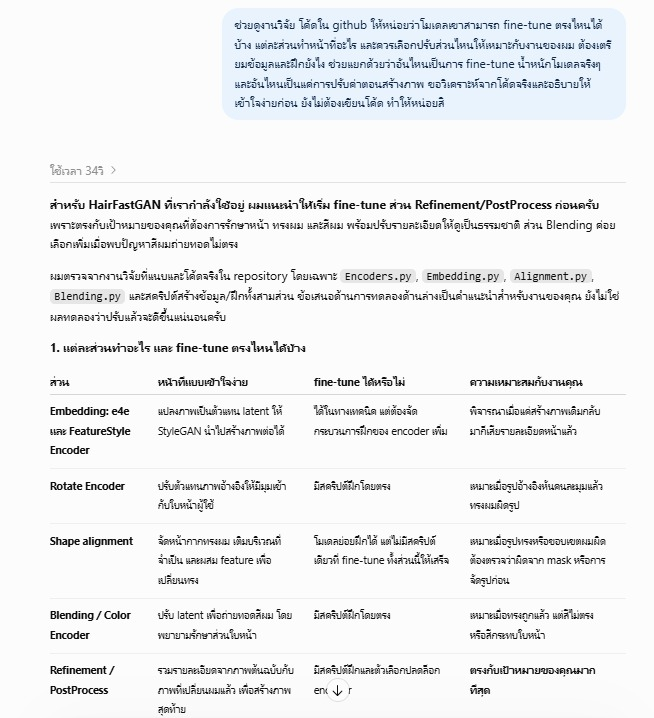
\includegraphics[width=0.6\textwidth]{images/ai_prompt_finetune.jpg}
\caption{ข้อความสั่งงานและตอนต้นของคำตอบ ChatGPT เรื่องส่วนที่ปรับจูนได้ของ HairFastGAN}
\label{fig:ai_finetune}
\par\vspace{3pt}{\footnotesize\raggedright หมายเหตุ: AI = Artificial Intelligence (ปัญญาประดิษฐ์), e4e = Encoder for Editing, CLIP = Contrastive Language-Image Pre-training, BiSeNet = Bilateral Segmentation Network, StyleGAN2 = Style-based Generative Adversarial Network รุ่นที่ 2\par}
\end{figure}

\begin{figure}[H]
\centering
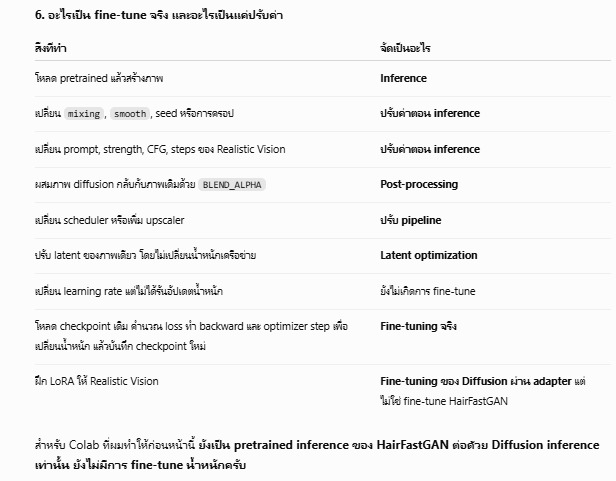
\includegraphics[width=0.6\textwidth]{images/ai_answer_ft_vs_infer.jpg}
\caption{ตารางในคำตอบของ ChatGPT ที่แยกการปรับจูนน้ำหนักจริงออกจากการปรับค่าตอนสร้างภาพ}
\label{fig:ai_ft_infer}
\par\vspace{3pt}{\footnotesize\raggedright หมายเหตุ: AI = Artificial Intelligence (ปัญญาประดิษฐ์), CFG = Classifier-Free Guidance, LoRA = Low-Rank Adaptation\par}
\end{figure}

คำตอบนี้มีประโยชน์ที่สุดในสามข้อ เพราะช่วยให้ผู้วิจัยเห็นภาพรวมของโค้ดและกำหนดขอบเขตงานได้
แต่ผู้วิจัยตรวจทุกประเด็นกับโค้ดจริงก่อน และตัดสินใจหลายเรื่องต่างจากที่ AI แนะนำ
เรื่องที่ผู้วิจัยใช้ตามคำตอบ ได้แก่ การแยกการปรับจูนจริงออกจากการปรับค่าตอนสร้างภาพ
การล็อกโมดูล Embedding, Pose และ Shape ไว้ การเลือก Checkpoint จากชุดตรวจสอบโดยดูหลายด้าน
และแนวคิดเทียบโมเดลทั้งก่อนและหลังต่อ Diffusion ซึ่งกลายเป็นโครงของแบบประเมินผู้ใช้
เรื่องที่ผู้วิจัยตรวจแล้วแก้ คือคำเตือนเรื่อง \texttt{strict=False}
ในโค้ดที่ใช้จริง ผู้วิจัยโหลดน้ำหนักด้วย \texttt{strict=True}
และตรวจว่าชื่อพารามิเตอร์ที่ฝึกตรงกับชั้น Modulation ของ Blending Encoder ครบทุกตัว
ส่วนเรื่องที่ผู้วิจัยทำต่างจากคำแนะนำมีสี่เรื่อง
เรื่องแรก ผู้วิจัยปรับจูนทั้ง Blending (เฉพาะชั้น Modulation) และ PostProcess ทั้งโมดูลพร้อมกัน
เพราะผลจากโมเดลตั้งต้นมีปัญหาทั้งสีผมที่เป็นปื้นและใบหน้าซีด
เรื่องที่สอง ผู้วิจัยใช้อัตราการเรียนรู้เท่ากับหรือต่ำกว่าที่ AI แนะนำ คือ $1 \times 10^{-5}$ และ $5 \times 10^{-6}$ สำหรับ Blending
และ $1 \times 10^{-6}$ และ $5 \times 10^{-7}$ สำหรับ PostProcess (ตารางที่~\ref{tab:trials})
เรื่องที่สาม ผู้วิจัยไม่ได้ใช้ฟังก์ชันสูญเสียเดิมของโครงการ แต่ออกแบบฟังก์ชันสูญเสีย 5 ด้านขึ้นเอง (หัวข้อที่~\ref{sec:loss})
และใช้ชุดเดียวกันกับ Barbershop เพื่อให้เปรียบเทียบสองโมเดลได้ยุติธรรม
เรื่องสุดท้าย ผู้วิจัยเพิ่มเกณฑ์ผ่าน 5 ด่านในการเลือก Checkpoint ซึ่งไม่มีในคำตอบของ AI
และขยายงานไปปรับจูน Barbershop ด้วย ซึ่งอยู่นอกขอบเขตของคำถามนี้

\section{การสร้าง Colab ทดลอง Barbershop แบบ Pretrained \mbox{(ChatGPT)}}
\label{sec:ai_bs_colab}

หลังได้ผลของ HairFastGAN แล้ว ผู้วิจัยต้องการรัน Barbershop แบบ Pretrained เพื่อใช้เป็นโมเดลเปรียบเทียบ
จึงแนบไฟล์งานวิจัย Barbershop (arXiv:2106.01505v2) ให้ ChatGPT และส่งข้อความดังนี้
\begin{quote}
\small ``ช่วยอ่านงานวิจัยที่แนบและโค้ดใน \url{https://github.com/ZPdesu/Barbershop}
แล้วทำไฟล์ Colab ให้ผมหน่อย ขอให้ติดตั้งและโหลดโมเดล pretrained มาใช้งานได้
อัปโหลดรูปหน้า รูปทรงผม และรูปสีผมเพื่อสร้างภาพผลลัพธ์ พร้อมบันทึกรูปได้
ขอแบบรันตามได้ตั้งแต่ต้นจนจบ พร้อมอธิบายขั้นตอนและสรุปการทำงานให้ผมเข้าใจง่าย ๆ ด้วยครับ''
\end{quote}

ChatGPT ตอบกลับเป็นไฟล์ \texttt{Barbershop\_Pretrained\_\allowbreak Thai\_Colab.ipynb} ดังภาพที่~\ref{fig:ai_bs_colab}
ในไฟล์ล็อกรุ่นของโค้ดจาก GitHub ไว้ ดาวน์โหลดน้ำหนัก StyleGAN2 กับ BiSeNet และโมเดลจุดสังเกตบนใบหน้า
จัดแนวใบหน้าเป็นภาพ $1024 \times 1024$ แล้วรันโค้ดของผู้พัฒนาตามลำดับ
คือค้นหารหัสใน $W^{+}$ ค้นหาต่อใน $FS$ จัดรูปตามหน้ากาก และผสมสไตล์
โดยมีโหมด \texttt{official} ที่ใช้จำนวนรอบตามค่าเริ่มต้นของโค้ด (1,100 / 250 / 140 / 100 / 400 รอบ)
และโหมด \texttt{preview} ที่ลดรอบไว้ทดสอบระบบเท่านั้น
ChatGPT ยังแก้โค้ดเดิมบางจุดให้รันบน Colab รุ่นปัจจุบันได้ เช่น คำสั่งย่อภาพของ Pillow ที่เลิกใช้แล้ว
การโหลดน้ำหนักด้วย PyTorch รุ่นใหม่ และการกันหารด้วยศูนย์เมื่อหน้ากากว่าง พร้อมบันทึกรายการที่แก้ไว้ในไฟล์แยก
และระบุว่ายังไม่ได้รันสร้างภาพจริงบน GPU

\begin{figure}[H]
\centering
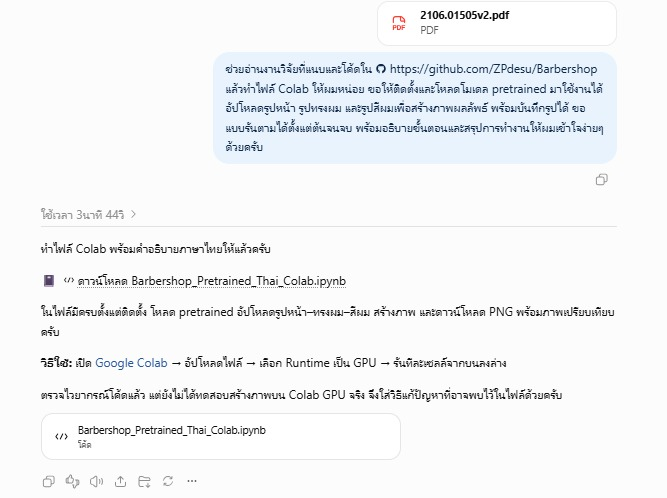
\includegraphics[width=0.6\textwidth]{images/ai_bs_prompt_colab.jpg}
\caption{ข้อความสั่งงานและคำตอบของ ChatGPT ในการสร้าง Colab สำหรับรัน Barbershop แบบ Pretrained}
\label{fig:ai_bs_colab}
\par\vspace{3pt}{\footnotesize\raggedright หมายเหตุ: GPU = Graphics Processing Unit (หน่วยประมวลผลกราฟิก), PNG = Portable Network Graphics (ไฟล์ภาพ)\par}
\end{figure}

ไฟล์นี้เป็นส่วนที่ผู้วิจัยนำไปใช้ต่อมากที่สุดในบรรดาคำตอบทั้งหมด แต่ก็ใช้หลังจากตรวจกับโค้ดต้นฉบับแล้ว
ผู้วิจัยเปิดไฟล์ \texttt{main.py} ใน GitHub เทียบว่าจำนวนรอบในโหมด \texttt{official} ตรงกับค่าเริ่มต้นจริง
และดูว่าการแก้โค้ดแต่ละจุดไม่ได้เปลี่ยนวิธีการของ Barbershop
จากนั้นนำไปรันจริง และใช้ค่าเดียวกันนี้ในขั้นทดลอง ได้แก่ จำนวนรอบตามค่าเริ่มต้นทั้งหมด
โหมด \texttt{realistic} ค่าเรียบของหน้ากาก 5 และการแก้การโหลดน้ำหนักกับคำสั่งย่อภาพแบบเดียวกัน
โหมด \texttt{preview} ผู้วิจัยไม่ได้ใช้กับผลที่รายงาน เพราะ ChatGPT เตือนไว้เองว่าไม่ควรใช้เป็นผลตั้งต้น
สิ่งที่ผู้วิจัยเขียนเพิ่มเองสำหรับการทดลอง คือให้รันการค้นหารหัสของแต่ละภาพเพียงครั้งเดียวแล้วเก็บไว้ใช้ซ้ำ
ตรวจว่าน้ำหนักตัวสร้างภาพไม่ถูกเปลี่ยนระหว่างรัน และจับเวลาของแต่ละขั้นแยกกัน

\section{การเพิ่มขั้นปรับภาพต่อจาก Barbershop \mbox{(ChatGPT)}}
\label{sec:ai_bs_diffusion}

เมื่อได้ภาพจาก Barbershop แล้ว ผู้วิจัยขอให้ ChatGPT เพิ่มขั้นปรับภาพต่อท้าย ด้วยข้อความเดียวกับที่ใช้กับ HairFastGAN
\begin{quote}
\small ``จากโค้ดเดิม ช่วยเพิ่มขั้นตอนปรับภาพด้วย Stable Diffusion โมเดล Realistic Vision V5.1
ต่อจากภาพผลลัพธ์ให้หน่อย อยากให้หน้าและเส้นผมดูคมชัดเป็นธรรมชาติมากขึ้น
โดยรักษาหน้าตา ทรงผม และสีผมจากภาพเดิมให้มากที่สุด แสดงภาพก่อนและหลังพร้อมเวลาประมวลผล
และบันทึกรูปได้ ทำเป็นเซลล์เพิ่มใน Colab ให้ด้วย''
\end{quote}

ChatGPT เพิ่มส่วนที่ 10 ต่อท้ายไฟล์เดิม ดังภาพที่~\ref{fig:ai_bs_diffusion}
แนวทางยังเป็น Image-to-Image ทั้งภาพเหมือนของ HairFastGAN แต่ค่าต่างออกไปเล็กน้อย
คือความแรง 0.15 ค่านำทาง 3.5 จำนวน 40 ขั้น และผสมภาพจาก Diffusion ร้อยละ 70 กับภาพเดิมร้อยละ 30
พร้อมแสดงภาพก่อนและหลัง แยกเวลาโหลดโมเดลออกจากเวลาปรับภาพ และเลือกบันทึกลง Google Drive ได้
ChatGPT ระบุไว้ว่ายังไม่ได้ทดสอบบน GPU จริง และข้อความ ``same person'' ในข้อความสั่งงานไม่ได้ล็อกใบหน้าให้เหมือนเดิม

\begin{figure}[H]
\centering
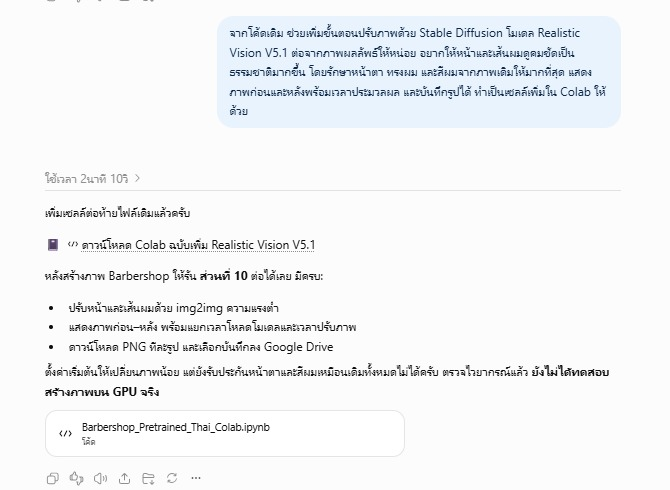
\includegraphics[width=0.6\textwidth]{images/ai_bs_prompt_diffusion.jpg}
\caption{ข้อความสั่งงานและคำตอบของ ChatGPT ในการเพิ่มขั้นปรับภาพต่อจาก Barbershop}
\label{fig:ai_bs_diffusion}
\par\vspace{3pt}{\footnotesize\raggedright หมายเหตุ: GPU = Graphics Processing Unit (หน่วยประมวลผลกราฟิก), PNG = Portable Network Graphics (ไฟล์ภาพ)\par}
\end{figure}

ผู้วิจัยไม่ได้ใช้ค่าชุดนี้ ปัญหาที่พบคือคำตอบของ ChatGPT ให้ค่าไม่เท่ากันระหว่างสองโมเดล
(HairFastGAN ความแรง 0.18 ผสม 0.65 แต่ Barbershop ความแรง 0.15 ผสม 0.70)
ถ้านำไปใช้ตรง ๆ จะเปรียบเทียบผลของ Diffusion ระหว่างสองโมเดลไม่ได้
ผู้วิจัยจึงใช้ขั้นขัดเกลาชุดเดียวกันกับภาพจากทั้งสองโมเดล ตามที่อธิบายในหัวข้อที่~\ref{sec:ai_diffusion}
คือ Inpainting เฉพาะผมกับใบหน้า ความแรง 0.15 ค่านำทาง 2.5 UniPC 30 ขั้น และ Seed 3407
สิ่งที่คงไว้จากคำตอบนี้คือแนวคิดแยกเวลาโหลดโมเดลออกจากเวลาประมวลผล และการเก็บภาพก่อนและหลังไว้เทียบกัน

\section{การวิเคราะห์ว่าส่วนไหนของ Barbershop ปรับจูนได้ \mbox{(ChatGPT)}}
\label{sec:ai_bs_finetune}

ผู้วิจัยถามคำถามเดียวกับหัวข้อที่~\ref{sec:ai_finetune} แต่เปลี่ยนเป็น Barbershop
เพราะต้องการรู้ว่าโมเดลที่ไม่มีเครือข่ายทายรหัสจะปรับจูนตรงไหนได้บ้าง
\begin{quote}
\small ``ช่วยดูงานวิจัย โค้ดใน github ให้หน่อยว่าโมเดลเขาสามารถ fine-tune ตรงไหนได้บ้าง
แต่ละส่วนทำหน้าที่อะไร และควรเลือกปรับส่วนไหนให้เหมาะกับงานของผม ต้องเตรียมข้อมูลและฝึกยังไง
ช่วยแยกด้วยว่าอันไหนเป็นการ fine-tune น้ำหนักโมเดลจริง ๆ และอันไหนเป็นแค่การปรับค่าตอนสร้างภาพ
ขอวิเคราะห์จากโค้ดจริงและอธิบายให้เข้าใจง่ายก่อน ยังไม่ต้องเขียนโค้ด''
\end{quote}

ChatGPT ตอบว่าประเด็นสำคัญที่สุดคือ Barbershop เดิมไม่ได้ปรับจูนน้ำหนักโมเดลเลย ดังภาพที่~\ref{fig:ai_bs_finetune}
แม้ในโค้ดจะมีการหาอนุพันธ์และตัวปรับค่าทำงานทุกรอบ แต่สิ่งที่ถูกปรับคือรหัสแฝงของแต่ละภาพ ส่วนน้ำหนักของ StyleGAN2 และ BiSeNet ถูกล็อกไว้
จากนั้นเสนอทางเลือกที่เป็นการปรับจูนจริง ได้แก่ ปรับจูน BiSeNet ปรับ StyleGAN2 บางส่วน
ปรับตัวสร้างภาพเฉพาะบุคคล (Pivotal Tuning Inversion: PTI) ฝึก LoRA ของ Realistic Vision หรือฝึกตัวเข้ารหัสเพิ่ม
ถ้าเลือกปรับ StyleGAN2 ChatGPT แนะนำให้เริ่มจากบล็อกช่วงหลังที่คุมรายละเอียด และล็อก Mapping Network กับบล็อกช่วงต้นไว้
ดังภาพที่~\ref{fig:ai_bs_stylegan} และเตือนว่าตัวสร้างภาพที่ปรับแล้วควรถูกใช้ตลอดทั้งกระบวนการ ตั้งแต่ขั้นค้นหารหัส
ChatGPT ยังแยกให้เห็นว่าการเปลี่ยนจำนวนรอบ อัตราการเรียนรู้ของการค้นหา หรือค่าของ Diffusion
เป็นเพียงการปรับค่า (Hyperparameter Tuning) ไม่ควรเรียกว่าการปรับจูนโมเดล
แนะนำให้แบ่งข้อมูลตามบุคคล และเสนอให้ตรวจว่าภาพเสียคุณภาพตั้งแต่ขั้นไหนก่อนเลือกส่วนที่จะฝึก

\begin{figure}[H]
\centering
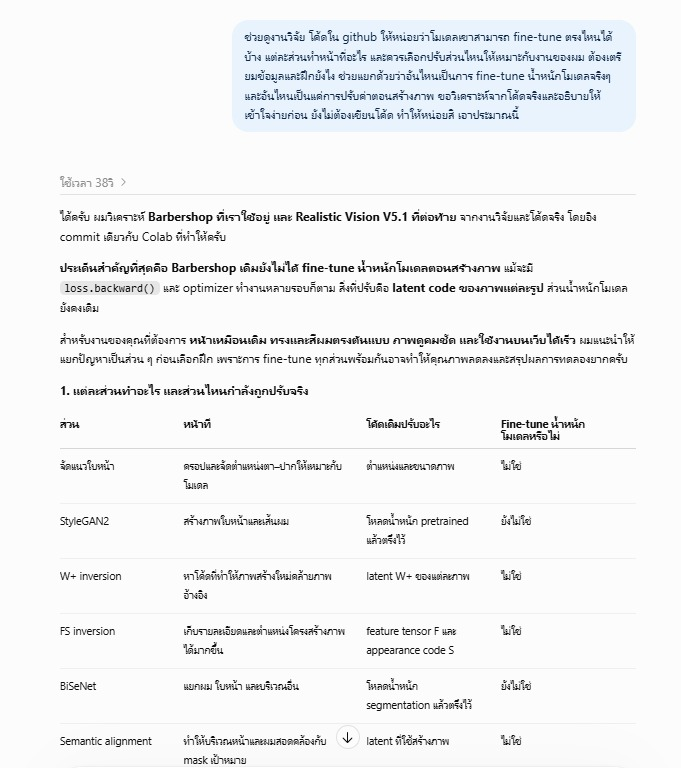
\includegraphics[width=0.6\textwidth]{images/ai_bs_prompt_finetune.jpg}
\caption{ข้อความสั่งงานและตอนต้นของคำตอบ ChatGPT เรื่องส่วนที่ปรับจูนได้ของ Barbershop}
\label{fig:ai_bs_finetune}
\par\vspace{3pt}{\footnotesize\raggedright หมายเหตุ: StyleGAN2 = Style-based Generative Adversarial Network รุ่นที่ 2, FS = พื้นที่แฝงที่แยกโครงร่าง ($F$) และสไตล์ ($S$), BiSeNet = Bilateral Segmentation Network\par}
\end{figure}

\begin{figure}[H]
\centering
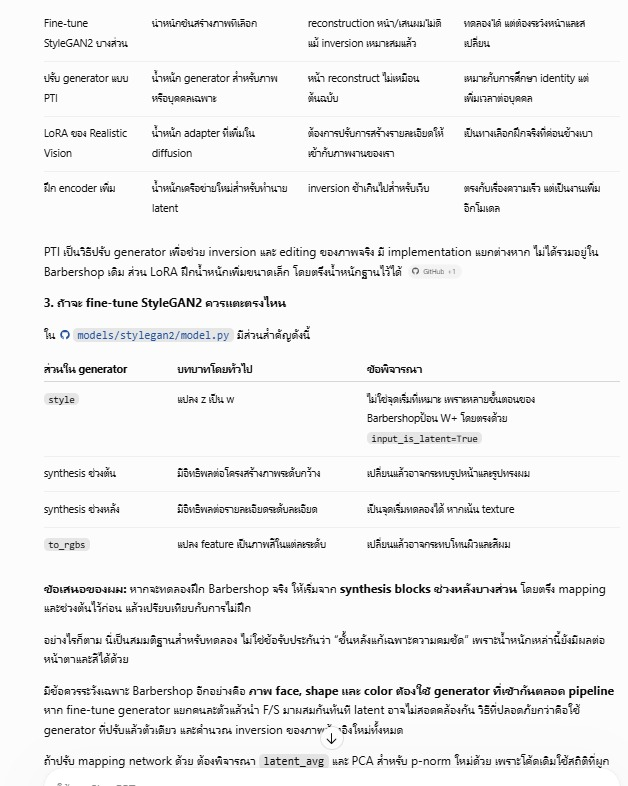
\includegraphics[width=0.55\textwidth]{images/ai_bs_answer_stylegan.jpg}
\caption{คำตอบของ ChatGPT เรื่องส่วนของ StyleGAN2 ที่ควรปรับจูนใน Barbershop}
\label{fig:ai_bs_stylegan}
\par\vspace{3pt}{\footnotesize\raggedright หมายเหตุ: PTI = Pivotal Tuning Inversion, LoRA = Low-Rank Adaptation, StyleGAN2 = Style-based Generative Adversarial Network รุ่นที่ 2\par}
\end{figure}

คำตอบนี้เป็นที่มาของการตัดสินใจหลักในการปรับจูน Barbershop
ผู้วิจัยตรวจกับไฟล์ \texttt{models/Net.py} แล้วพบว่าน้ำหนักของตัวสร้างภาพถูกตั้งไม่ให้รับเกรเดียนต์จริงตามที่ ChatGPT บอก
จึงเลือกทางเลือกปรับ StyleGAN2 บางส่วนตามคำแนะนำ โดยปรับเฉพาะชั้น \texttt{convs[6:]} และ \texttt{to\_rgbs[3:]}
ซึ่งเป็นชั้นความละเอียด 64--1024 พิกเซล และล็อก Mapping Network กับชั้นช่วงต้นไว้ (หัวข้อที่~\ref{sec:pipe_bs})
ส่วนที่ผู้วิจัยทำต่างจากคำแนะนำมีสองเรื่อง
เรื่องแรก ระหว่างฝึกผู้วิจัยไม่ได้ค้นหารหัสใหม่ด้วยตัวสร้างภาพที่ปรับแล้วทุกรอบ แต่ใช้รหัสที่ค้นไว้ครั้งเดียวจากตัวสร้างภาพเดิม
เพราะถ้าค้นใหม่ทุกรอบ การฝึกหนึ่ง Trial จะใช้เวลาหลายสัปดาห์ ผู้วิจัยยอมรับข้อจำกัดนี้และเขียนไว้ในบทที่ 3
แต่ตอนทดสอบและสร้างภาพให้ผู้ใช้ประเมิน ผู้วิจัยรวมน้ำหนักที่ปรับแล้วเข้ากับไฟล์ \texttt{ffhq.pt}
และใช้ตัวสร้างภาพตัวนี้ตลอดทั้งกระบวนการตามที่ ChatGPT เตือน
เรื่องที่สอง ผู้วิจัยไม่ได้ทำทางเลือกอื่น เช่น PTI หรือ LoRA เพราะต้องการให้ Barbershop ใช้ฟังก์ชันสูญเสีย
ชุดข้อมูล และกติกาการเลือก Checkpoint ชุดเดียวกับ HairFastGAN เพื่อให้เปรียบเทียบได้ตรงกัน
การแยกการปรับจูนจริงออกจากการปรับค่าตามคำตอบนี้ ทำให้ผู้วิจัยรายงานในบทที่ 3 ได้ชัดว่า
จำนวนรอบค้นหาทั้งหมดใช้ค่าเดิมของผู้พัฒนา และสิ่งที่ถูกฝึกจริงมีเพียงชั้นของ StyleGAN2 ที่ระบุไว้

\section{การเปรียบเทียบ Barbershop A30 กับ HairFastGAN B24 \mbox{(ChatGPT)}}
\label{sec:ai_compare}

หลังปรับจูนเสร็จและเลือก Checkpoint ได้แล้ว ผู้วิจัยต้องการเครื่องมือที่สร้างภาพจากสองโมเดลด้วยภาพนำเข้าชุดเดียวกัน
ต่อด้วยขั้นขัดเกลาชุดเดียวกัน แล้ววัดผลทุกขั้น จึงส่งไฟล์เปรียบเทียบเดิมของโครงการให้ ChatGPT พร้อมข้อความดังนี้
\begin{quote}
\small ``หลังจาก fine-tune เสร็จแล้ว ช่วยทำไฟล์ Colab เปรียบเทียบ Barbershop ที่ใช้ checkpoint A30
กับ HairFastGAN ที่ใช้ checkpoint B24 ให้หน่อย โดยใช้รูปหน้า รูปทรงผม และรูปสีผมชุดเดียวกัน
แล้วนำผลของทั้งสองโมเดลไปต่อ Diffusion Realistic Vision V5.1 และปรับความคมด้วยวิธีและค่าเดียวกัน
แสดงภาพแต่ละขั้นตอน พร้อมเปรียบเทียบเวลาและประเมินคุณภาพภาพ การรักษาใบหน้า ทรงผม และสีผม
สรุปเป็นตารางกับกราฟ พร้อมบันทึกภาพและผลประเมินได้ ขอแบบรันตามได้ตั้งแต่ต้นจนจบ พร้อมอธิบายให้เข้าใจง่าย ๆ''
\end{quote}

ChatGPT ตอบกลับเป็นไฟล์ \texttt{Barbershop\_A30\_vs\_\allowbreak HairFastGAN\_B24\_\allowbreak Complete.ipynb} ดังภาพที่~\ref{fig:ai_compare}
ไฟล์นี้ต่อยอดจากไฟล์เปรียบเทียบเดิมของโครงการ ไม่ได้เขียนวิธีการใหม่
ส่วนที่ ChatGPT เพิ่มคือการตรวจไฟล์น้ำหนัก A30 ก่อนใช้ โดยดูเลข Epoch ชื่อและขนาดของพารามิเตอร์
ว่ามีเฉพาะชั้นที่ปรับจูนจริง แล้วรวมเข้ากับ \texttt{ffhq.pt} เป็นไฟล์ใหม่ และบันทึกค่าแฮชของทั้งไฟล์ A30 และไฟล์ที่รวมแล้วไว้ในบันทึกการรัน
ด้านการวัดผล ไฟล์วัดภาพทั้ง 8 ภาพ (2 โมเดล $\times$ 4 ขั้น) ด้วย MUSIQ ArcFace ความคลาดเคลื่อนสีผมในปริภูมิ Lab
IoU ของผมเทียบกับภาพก่อน Diffusion และ MAE กับ SSIM นอกหน้ากาก แยกผลต่างเป็น 4 ช่วง
จับเวลาแต่ละขั้นแยกกัน และมีส่วนเลือกจับเวลาขั้นขัดเกลาซ้ำหลายรอบ
ChatGPT อธิบายข้อจำกัดของตัวชี้วัดไว้ด้วย เช่น MUSIQ ไม่ได้บอกว่าทรงผมถูกต้อง IoU เทียบภาพก่อน Diffusion ไม่ใช่การวัดว่าตรงทรงเป้าหมาย
และผลจากภาพชุดเดียวยังสรุปเป็นผลวิจัยไม่ได้ และแจ้งว่าตรวจเพียงไวยากรณ์ของโค้ด ยังไม่ได้รันกับน้ำหนักจริงบน GPU

\begin{figure}[H]
\centering
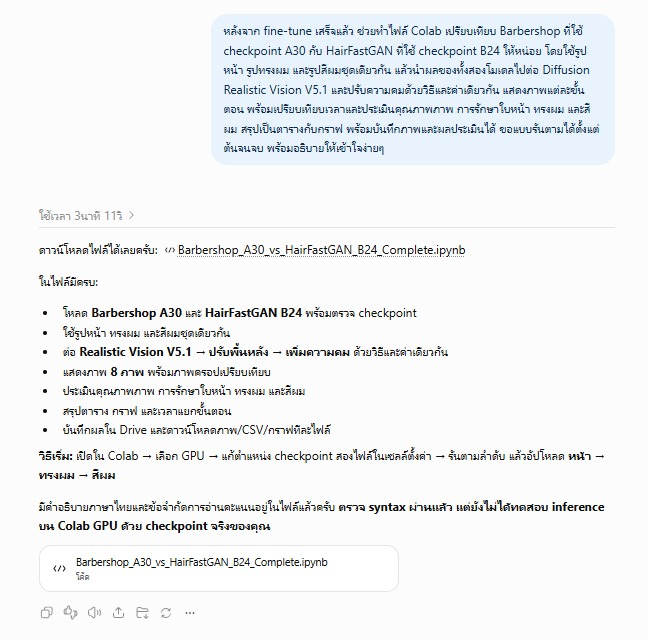
\includegraphics[width=0.55\textwidth]{images/ai_compare_prompt.jpg}
\caption{ข้อความสั่งงานและคำตอบของ ChatGPT ในการสร้างไฟล์เปรียบเทียบ Barbershop A30 กับ HairFastGAN B24}
\label{fig:ai_compare}
\par\vspace{3pt}{\footnotesize\raggedright หมายเหตุ: A30 = น้ำหนักของ Barbershop-FT Trial A Epoch 30, B24 = น้ำหนักของ HairFastGAN Trial B Epoch 24, CSV = Comma-Separated Values (ไฟล์ตาราง), PNG = Portable Network Graphics (ไฟล์ภาพ), GPU = Graphics Processing Unit (หน่วยประมวลผลกราฟิก)\par}
\end{figure}

ก่อนใช้ ผู้วิจัยตรวจว่าค่าของขั้นขัดเกลาในไฟล์ตรงกับที่ตั้งไว้ในบทที่ 3 ทุกค่า
ได้แก่ Seed 3407 ความแรง 0.15 จำนวน 30 ขั้น ค่านำทาง 2.5 และน้ำหนักเพิ่มความคมของผม 0.65 ใบหน้า 0.25 จำกัด $\pm 5$ ระดับ
และตรวจว่าทั้งสองโมเดลใช้ภาพที่จัดแนวแล้วชุดเดียวกัน
ผลกรณีศึกษาในหัวข้อที่~\ref{sec:diff_result} ใช้ตัวชี้วัดและการแยกเวลาชุดเดียวกับไฟล์นี้
และผู้วิจัยตีความผลตามข้อจำกัดที่ ChatGPT เตือนไว้ คือรายงานเป็นกรณีศึกษา 8 ชุดภาพ ไม่สรุปเป็นผลทั่วไป
และไม่ใช้ MUSIQ หรือ IoU เทียบภาพก่อนเป็นตัวตัดสินคุณภาพของทรงผม
ส่วนที่ผู้วิจัยทำเพิ่มเองคือรันกับภาพ 8 ชุด รวมใบหน้า 7 คน และสรุปผลเป็นรายชุดพร้อมค่าเฉลี่ย
นำตัวเลขทั้งหมดมาจากไฟล์ผลลัพธ์ที่บันทึกไว้โดยตรง และใช้ความเห็นของผู้ใช้ 41 คนเป็นหลักในการตัดสินว่าภาพดีขึ้นหรือไม่

\section{การออกแบบหน้าเว็บ LOOKLAB \mbox{(ChatGPT)}}
\label{sec:ai_web_design}

เมื่อโมเดลพร้อมใช้งานแล้ว ผู้วิจัยต้องการหน้าเว็บที่ดูดีและใช้ง่ายสำหรับให้คนทั่วไปทดลอง
แต่ยังไม่มีภาพในใจว่าหน้าเว็บควรเป็นแบบไหน จึงขอให้ ChatGPT ออกแบบหน้าตาเว็บมาให้เลือกก่อน
\begin{quote}
\small ``ช่วยออกแบบเว็บให้ใช้งานสวย ๆ ให้หน่อย เปลี่ยนชื่อเป็น LOOKLAB ออกเป็นรูปหน้าเว็บมาให้ดูก่อน
ออกแบบหน้าเว็บหลายแบบให้เลือกสิ ขอสัก 10 หน้า''
\end{quote}

ChatGPT ตอบกลับเป็นภาพตัวอย่างหน้าเว็บ 10 แบบ ดังภาพที่~\ref{fig:ai_web_design}
แต่ละแบบใช้ชุดสีและการจัดวางต่างกัน และ ChatGPT สรุปชื่อกับแนวของแต่ละแบบเป็นตาราง ดังภาพที่~\ref{fig:ai_web_10styles}
เช่น แบบ 01 Rose Atelier โทนชมพูกุหลาบ แบบ 03 Peach Room โทนพีช--คอรัล อบอุ่น และแบบ 08 Nordic Blue โทนฟ้าหม่น
ChatGPT ระบุไว้ว่าทั้งหมดเป็นภาพแนวทางการออกแบบเท่านั้น ยังไม่ได้แก้โค้ด
และแนะนำว่าเลือกแบบเดียว หรือผสมสีกับการจัดวางจากหลายแบบก็ได้

\begin{figure}[H]
\centering
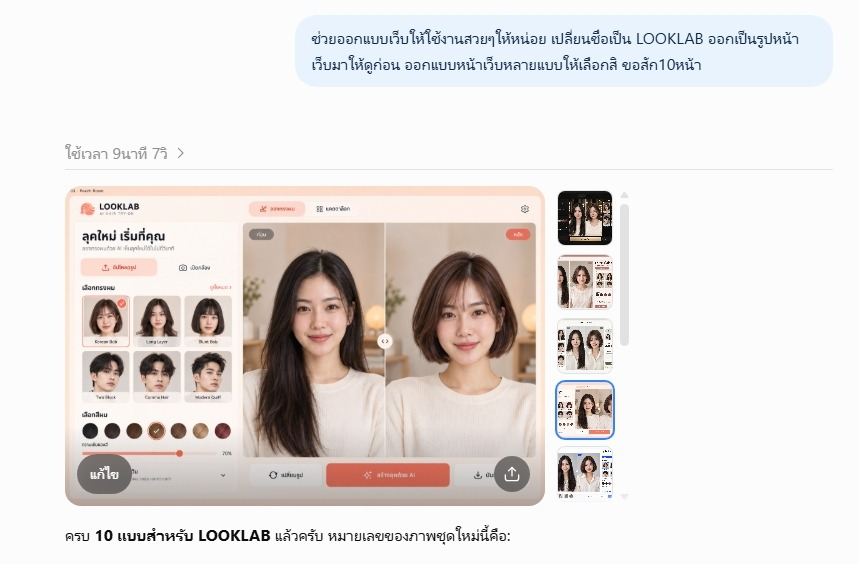
\includegraphics[width=0.6\textwidth]{images/ai_web_design.jpg}
\caption{ข้อความสั่งงานและภาพตัวอย่างหน้าเว็บที่ ChatGPT ออกแบบ (แบบ 03 Peach Room)}
\label{fig:ai_web_design}
\end{figure}

\begin{figure}[H]
\centering
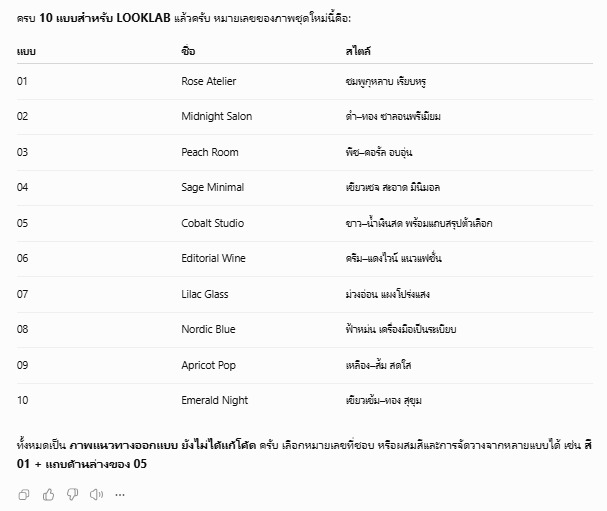
\includegraphics[width=0.55\textwidth]{images/ai_web_10styles.jpg}
\caption{ตารางสรุปหน้าเว็บ 10 แบบที่ ChatGPT ออกแบบให้เลือก}
\label{fig:ai_web_10styles}
\end{figure}

ผู้วิจัยใช้ภาพชุดนี้เป็นตัวเลือกด้านหน้าตาเท่านั้น โดยดูทั้ง 10 แบบแล้วเลือกแบบ 03 Peach Room
เพราะโทนพีช--คอรัลดูอบอุ่นและเป็นมิตรกับผู้ใช้ทั่วไป และการจัดวางแบ่งเป็นแผงเลือกทรงและสีด้านซ้ายกับภาพผลลัพธ์ด้านขวา
ซึ่งตรงกับลำดับการใช้งานของเว็บ คืออัปโหลดรูป เลือกทรง เลือกสี แล้วสร้างภาพ
ภาพตัวอย่างใช้ภาพบุคคลและผลลัพธ์ที่ ChatGPT สร้างขึ้นเพื่อแสดงแนวการออกแบบ ผู้วิจัยจึงไม่ได้นำภาพเหล่านี้ไปใส่ในเว็บ
ภาพทรงผม ภาพสีผม และภาพผลลัพธ์บนเว็บจริงมาจากชุดภาพของโครงการและจากโมเดลที่ทำงานจริงทั้งหมด

\section{การเขียนข้อความสั่งงานเพื่อสร้างหน้าเว็บจริง \mbox{(ChatGPT)}}
\label{sec:ai_web_prompt}

หลังเลือกแบบได้แล้ว ผู้วิจัยต้องนำแบบนี้ไปสร้างเป็นหน้าเว็บจริงใน Google AI Studio ซึ่งเป็นเครื่องมือที่ใช้พัฒนาโปรเจกต์เว็บของโครงการ
จึงถาม ChatGPT ว่าควรสั่งงานอย่างไร
\begin{quote}
\small ``ชอบ 03 Peach Room พีช--คอรัล อบอุ่น จะเอาไป prompt บอกให้ google ai studio ทำให้ได้แบบนี้ได้ยังไง''
\end{quote}

ChatGPT ตอบกลับเป็นข้อความสั่งงานสำเร็จรูปให้นำไปวางใน Google AI Studio พร้อมแนบภาพแบบ 03 ดังภาพที่~\ref{fig:ai_web_prompt}
ข้อความนี้กำหนดแนวการออกแบบเป็นค่าที่ชัดเจน เช่น พื้นหลังครีม \#FFF8F4 สีหลักคอรัล \#F27D68 พื้นสีอ่อน \#FFE9E1
ข้อความสีเข้ม \#392A25 เส้นขอบ \#EFDCD3 มุมการ์ดโค้ง 20--24 พิกเซล และฟอนต์ Noto Sans Thai
กำหนดการจัดวางหน้าคอมพิวเตอร์เป็นสองคอลัมน์ ด้านซ้ายประมาณร้อยละ 36 สำหรับอัปโหลดรูป เลือกทรง และเลือกสี
ด้านขวาประมาณร้อยละ 64 สำหรับภาพผู้ใช้ ตัวเลื่อนเทียบก่อนและหลัง และปุ่ม ``สร้างลุคด้วย AI''
และกำหนดลำดับการแสดงผลบนมือถือ
ส่วนที่สำคัญที่สุดคือข้อความนี้สั่งให้รักษาฟังก์ชันเดิมทั้งหมด ได้แก่ การอัปโหลด กล้อง AR การเลือกทรงและสี
การเชื่อมต่อ HairFastGAN ผ่าน API การตั้งค่าเซิร์ฟเวอร์ การดาวน์โหลด และคีย์ localStorage เดิม
ห้ามนำภาพหน้าจอมาวางแทนหน้าเว็บ และเมื่อแก้เสร็จต้อง build ตรวจ TypeScript และตรวจหน้าจอทั้งคอมพิวเตอร์และมือถือ

\begin{figure}[H]
\centering
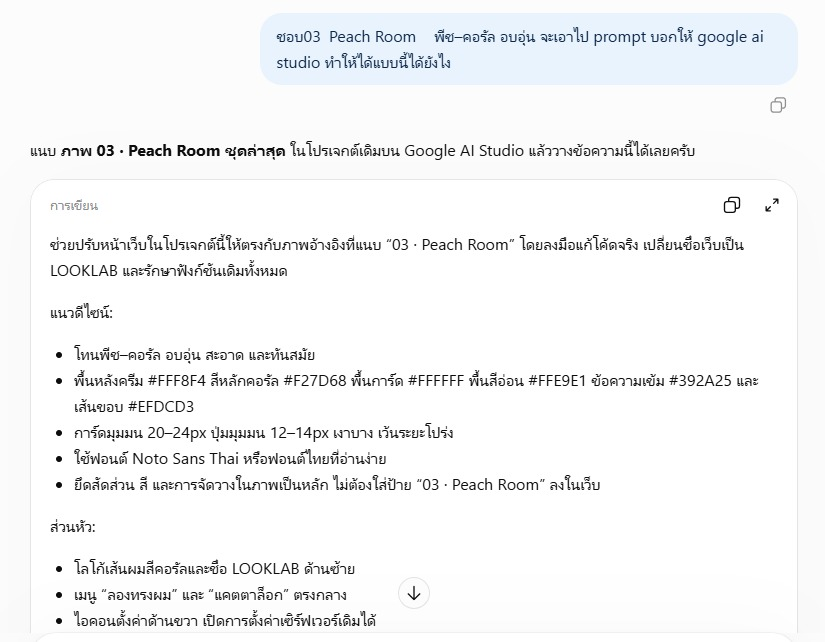
\includegraphics[width=0.6\textwidth]{images/ai_web_prompt.jpg}
\caption{ข้อความสั่งงานและข้อความสำหรับ Google AI Studio ที่ ChatGPT เขียนให้}
\label{fig:ai_web_prompt}
\par\vspace{3pt}{\footnotesize\raggedright หมายเหตุ: AI = Artificial Intelligence (ปัญญาประดิษฐ์), \#FFF8F4, \#F27D68 และอื่น ๆ = รหัสสีแบบเลขฐานสิบหก (Hex Color Code)\par}
\end{figure}

ผู้วิจัยนำข้อความนี้ไปใช้กับ Google AI Studio โดยไม่ได้แก้ข้อความ เพราะระบุสิ่งที่ต้องการได้ชัดกว่าที่ผู้วิจัยเขียนเอง
โดยเฉพาะส่วนที่สั่งให้รักษาฟังก์ชันเดิม ซึ่งผู้วิจัยใช้เป็นรายการตรวจผลที่ได้ในหัวข้อถัดไป
ผลที่ได้จาก Google AI Studio และสิ่งที่ผู้วิจัยตรวจพบอธิบายไว้ในหัวข้อที่~\ref{sec:ai_studio}

\section{การสร้างหน้าเว็บตามแบบที่เลือก \mbox{(Google AI Studio)}}
\label{sec:ai_studio}

ผู้วิจัยนำข้อความสั่งงานที่ ChatGPT เขียนให้ในหัวข้อที่~\ref{sec:ai_web_prompt} ไปวางใน Google AI Studio
พร้อมแนบภาพแบบ 03 Peach Room และพิมพ์ต่อท้ายว่า
\begin{quote}
\small ``เริ่มแก้โปรเจกต์ได้เลย ขอให้ใกล้ภาพอ้างอิงมากที่สุด ทั้งสี สัดส่วน รูปภาพ การ์ด และตำแหน่งปุ่ม''
\end{quote}

Google AI Studio ใช้โมเดล Gemini ทำงานประมาณ 14 นาที แก้ไฟล์ 18 ไฟล์ และได้หน้าเว็บตามภาพที่~\ref{fig:ai_studio}
หน้าตาที่ได้ใกล้กับแบบที่เลือกมาก ทั้งชุดสี การ์ดมุมโค้ง แผงเลือกทรงและสีด้านซ้าย และตัวเลื่อนเทียบก่อนและหลังด้านขวา
โค้ดใช้ค่าสีตามข้อความสั่งงานครบ คือ \#FFF8F4 \#F27D68 \#FFE9E1 \#392A25 และ \#EFDCD3 กับฟอนต์ Noto Sans Thai

\begin{figure}[H]
\centering
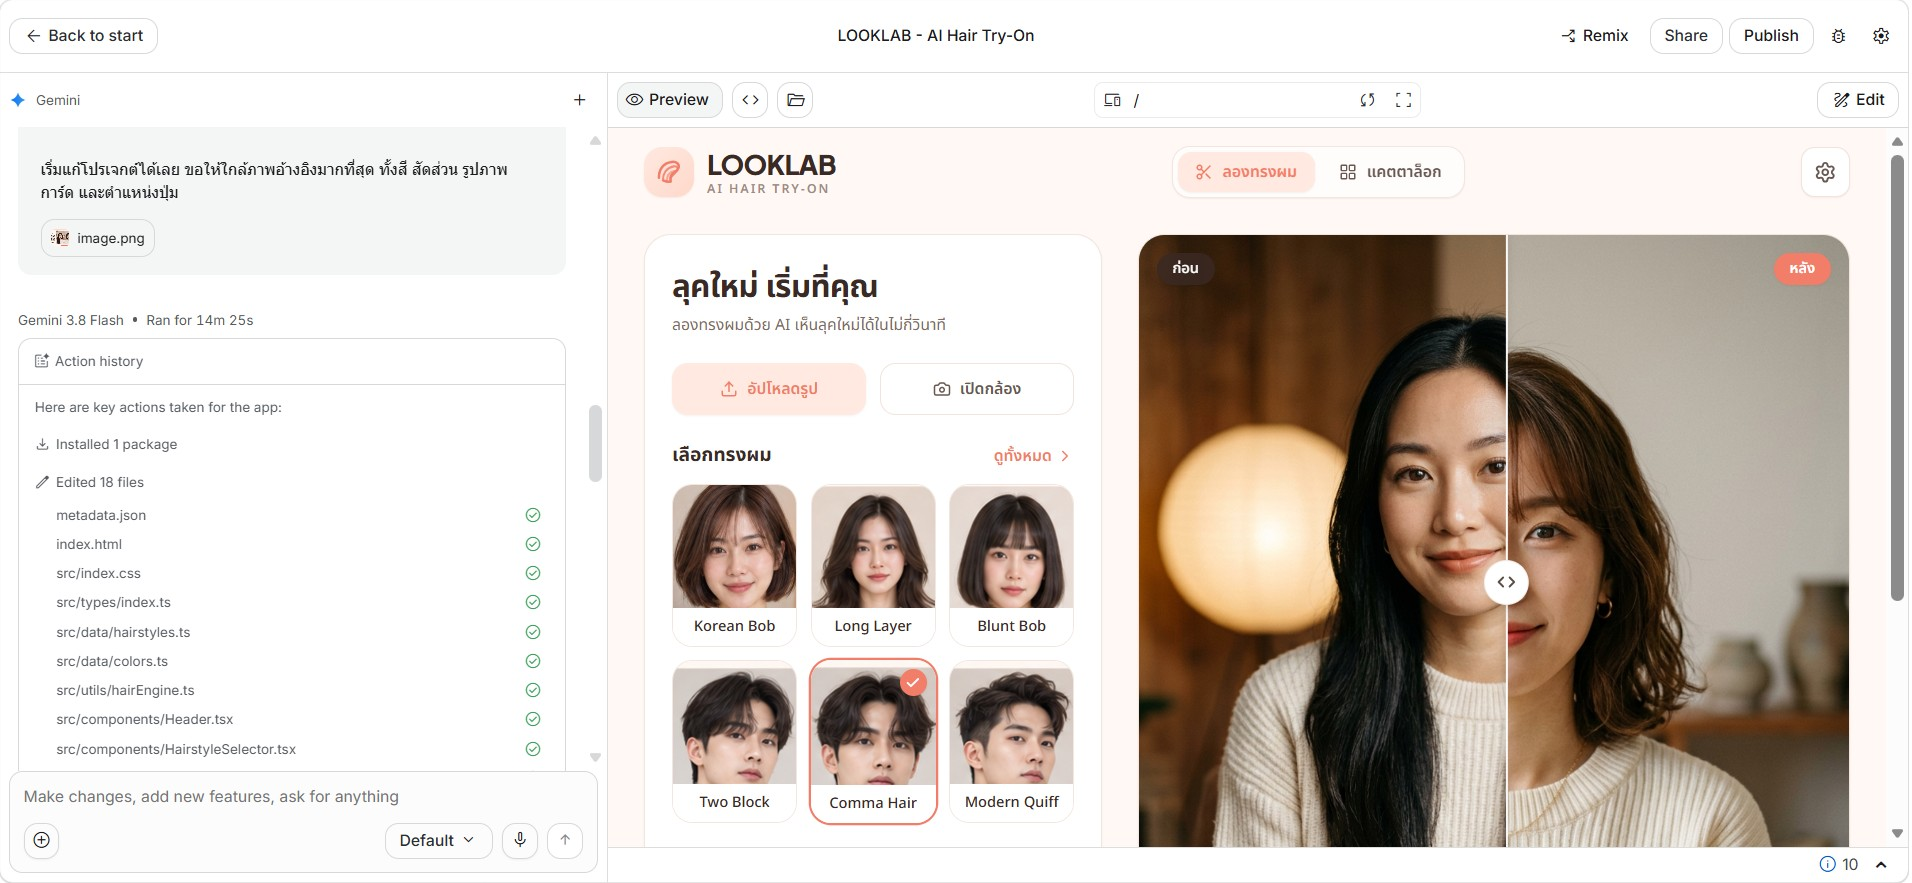
\includegraphics[width=\textwidth]{images/ai_studio_result.jpg}
\caption{หน้าเว็บที่ Google AI Studio สร้างตามข้อความสั่งงานและแบบ 03 Peach Room}
\label{fig:ai_studio}
\par\vspace{3pt}{\footnotesize\raggedright หมายเหตุ: AI = Artificial Intelligence (ปัญญาประดิษฐ์)\par}
\end{figure}

แม้หน้าตาจะตรงกับที่ต้องการ แต่เมื่อผู้วิจัยเปิดโค้ดเทียบกับโปรเจกต์เดิม กลับพบว่า Google AI Studio ไม่ได้แก้แค่หน้าตา
แต่เขียนโครงสร้างของเว็บขึ้นใหม่ และทำให้ฟังก์ชันเดิมหายไปหลายส่วน ทั้งที่ข้อความสั่งงานกำหนดให้รักษาไว้ทั้งหมด
ความต่างหลักสรุปไว้ในตารางที่~\ref{tab:ai_studio_compare}
คอลัมน์กลางคือโค้ดที่ Google AI Studio สร้าง และคอลัมน์ขวาคือเว็บ LOOKLAB ที่ใช้จริง

\begin{table}[H]
\centering
\caption{เปรียบเทียบโค้ดที่ Google AI Studio สร้างกับเว็บ LOOKLAB ที่ใช้จริง}
\label{tab:ai_studio_compare}
\small
\begin{tabular}{|L{3.4cm}|L{4.8cm}|L{4.8cm}|}
\hline
\textbf{รายการ} & \textbf{โค้ดจาก Google AI Studio} & \textbf{เว็บ LOOKLAB ที่ใช้จริง} \\ \hline
หน้าตาและชุดสี & ตามแบบ 03 Peach Room & ตามแบบ 03 Peach Room (สีข้อความปรับเป็น \#432B25) \\ \hline
จำนวนทรงผม & 10 ทรง (ภาพที่ AI สร้างขึ้น) & 24 ทรง จากชุดภาพของโครงการ \\ \hline
จำนวนสีผม & 7 สี & 28 สี และตัวเลือกสีธรรมชาติ \\ \hline
โหมดกล้อง & เปิดกล้องได้ แต่ไม่มีการติดตามใบหน้า & ติดตามใบหน้าด้วย MediaPipe FaceLandmarker และวางทรงผมแบบ AR \\ \hline
การเชื่อมต่อโมเดล & เรียกเซิร์ฟเวอร์โดยตรง ไม่มีเซิร์ฟเวอร์กลาง & ผ่านเซิร์ฟเวอร์กลาง Express ไปยัง FastAPI บน GPU และติดตามสถานะงาน \\ \hline
เมื่อเชื่อมต่อเซิร์ฟเวอร์ไม่ได้ & แต่งสีผมบนภาพด้วย Canvas หรือแสดงภาพตัวอย่าง แล้วแจ้งว่าสร้างสำเร็จ & แจ้งข้อผิดพลาดเป็นภาษาไทย ไม่แสดงภาพที่ไม่ได้มาจากโมเดล \\ \hline
แบบประเมินหลังใช้งาน & ไม่มี & มีแบบประเมิน 6 หัวข้อ และขอความยินยอม \\ \hline
คีย์ localStorage & เปลี่ยนเป็นชุดใหม่ & ใช้คีย์เดิม \\ \hline
\end{tabular}
\par\vspace{3pt}{\footnotesize\raggedright หมายเหตุ: AI = Artificial Intelligence (ปัญญาประดิษฐ์), AR = Augmented Reality (ความเป็นจริงเสริม), GPU = Graphics Processing Unit (หน่วยประมวลผลกราฟิก), API = Application Programming Interface, localStorage = พื้นที่เก็บข้อมูลในเบราว์เซอร์\par}
\end{table}

ปัญหาที่ร้ายแรงที่สุดคือแถวที่หก เมื่อไม่ได้ตั้งค่าเซิร์ฟเวอร์ หรือเชื่อมต่อเซิร์ฟเวอร์ไม่ได้
โค้ดของ Google AI Studio จะหน่วงเวลา 0.8 วินาทีให้ดูเหมือนกำลังประมวลผล แล้วระบายสีทับบริเวณผมด้วย Canvas
หรือแสดงภาพตัวอย่างที่เตรียมไว้ และถ้าไม่ได้ตั้งค่าเซิร์ฟเวอร์ ยังแจ้งผู้ใช้ว่าสร้างลุคสำเร็จ
ถ้านำขึ้นเว็บทั้งแบบนี้ ผู้ใช้อาจได้ภาพที่ไม่ได้มาจาก HairFastGAN เลยโดยไม่รู้ตัว
และคะแนนประเมินจากการทดลองใช้ 100 ครั้งก็จะไม่ได้วัดโมเดลของโครงการจริง

ผู้วิจัยจึงไม่ได้ใช้โค้ดชุดนี้แทนโปรเจกต์เดิม แต่ใช้เป็นต้นแบบด้านหน้าตาเท่านั้น
โดยนำชุดสี ฟอนต์ ขนาดมุมโค้ง และการจัดวางแบบสองคอลัมน์มาปรับเข้ากับโค้ดเดิมของ LOOKLAB
และคงทุกส่วนที่ทำงานจริงไว้ ได้แก่ ทรงผม 24 แบบ สีผม 28 สี โหมดกล้องที่ติดตามใบหน้า เซิร์ฟเวอร์กลางที่เชื่อมกับโมเดล
แบบประเมินหลังใช้งาน และคีย์ localStorage เดิม
เมื่อเชื่อมต่อเซิร์ฟเวอร์ไม่ได้ เว็บที่ใช้จริงจะแจ้งข้อผิดพลาด ไม่สร้างภาพขึ้นเอง
หน้าเว็บสุดท้ายแสดงในภาพที่~\ref{fig:web_main} (หัวข้อที่~\ref{sec:webapp})
ซึ่งหน้าตาใกล้กับภาพที่~\ref{fig:ai_studio} แต่ทุกภาพผลลัพธ์มาจากโมเดลของโครงการ

\section{การนำเว็บขึ้นใช้งานบน Vercel และ RunPod \mbox{(Claude)}}
\label{sec:ai_deploy}

ช่วงทดสอบแรก เซิร์ฟเวอร์โมเดลรันอยู่บน Google Colab และเชื่อมกับเว็บผ่าน ngrok ซึ่งต้องเปิด Colab ค้างไว้ตลอด
ผู้วิจัยจึงต้องการย้ายหน้าเว็บไปไว้บน Vercel และย้ายเซิร์ฟเวอร์โมเดลไปไว้บน RunPod ซึ่งเป็นบริการเช่า GPU
โดยให้เซิร์ฟเวอร์ใช้กระบวนการจากสมุดบันทึก \texttt{LOOKLAB\_Diffusion\_\allowbreak Native\_Sharp.ipynb} ที่ผู้วิจัยใช้อยู่
จึงแนบสมุดบันทึกนั้น โค้ดเซิร์ฟเวอร์เดิม (\texttt{khem\_backend.zip}) และโค้ดเว็บ (\texttt{looklab\_final.zip}) ให้ Claude พร้อมข้อความดังนี้
\begin{quote}
\small ``เราอยากเอา frontend ไปขึ้น vercel แล้วเอา backend ไปรันในรันพอต
โดยเปลี่ยนไปใช้โหลดจากไฟล์ LOOKLAB\_Diffusion\_Native\_Sharp.ipynb ของเราเอาไปแทนอันเดิม
ทำให้หน่อยสิให้มันเอาไปใช้ให้ได้ ต้องไปทำยังไงบ้างทำให้ทุกขั้นตอนตั้งแต่จนเสร็จ''
\end{quote}

Claude ตอบกลับเป็นไฟล์ \texttt{looklab\_deploy.zip} และคู่มือภาษาไทย \texttt{DEPLOY\_TH.md} ดังภาพที่~\ref{fig:ai_claude_deploy} และ~\ref{fig:ai_claude_steps}
ในไฟล์แบ่งเป็นสองส่วน ส่วนแรกคือเซิร์ฟเวอร์โมเดลที่ย้ายโค้ดจากสมุดบันทึกมาเป็น Docker Image สำหรับ RunPod
โดยตรวจค่าแฮชของไฟล์น้ำหนัก B24 ก่อนเริ่มทำงาน ใช้ค่าขั้นขัดเกลาเดิม (ความแรง 0.15, 30 ขั้น, ค่านำทาง 2.5, Seed 3407)
และมีเส้นทาง \texttt{/generate}, \texttt{/health} และ \texttt{/feedback} เหมือนเดิม พร้อมเพิ่ม \texttt{/ping} ที่ RunPod ใช้ตรวจสถานะ
ส่วนที่สองคือหน้าเว็บสำหรับ Vercel ที่เปลี่ยนเซิร์ฟเวอร์กลาง Express เป็น Vercel Functions แยกไฟล์ในโฟลเดอร์ \texttt{api/}
เก็บ API key ของ RunPod ไว้ฝั่งเซิร์ฟเวอร์ ย่อรูปไม่ให้เกินด้านยาว 1,536 พิกเซลก่อนส่ง เพราะ Vercel รับข้อมูลได้ไม่เกิน 4.5 MB ต่อครั้ง
และลองเชื่อมต่อใหม่อัตโนมัติระหว่างรอเซิร์ฟเวอร์เริ่มทำงาน (Cold Start)
Claude ยังพบว่ารูปสีผม 28 รูปในเว็บเดิมเป็นภาพเส้นผมล้วนที่ไม่มีใบหน้า ทำให้ HairFastGAN หาใบหน้าไม่เจอทุกครั้งที่เลือกสีอื่นนอกจากสีธรรมชาติ
จึงเพิ่มขั้นสำรองที่ย้อมผมในรูปของผู้ใช้ด้วยสีจากภาพนั้นแล้วใช้เป็นภาพอ้างอิงสีแทน
และเตือนว่าไฟล์ \texttt{.env} ในโค้ดเซิร์ฟเวอร์เดิมมี API key จริงอยู่ ควรสร้าง key ใหม่
Claude แจ้งว่าทดสอบฟังก์ชันประมวลผลภาพ เส้นทาง API และการ build บน Vercel แล้ว
แต่ยังไม่ได้ build Docker Image จริงและยังไม่ได้รันโมเดลบน GPU

\begin{figure}[H]
\centering
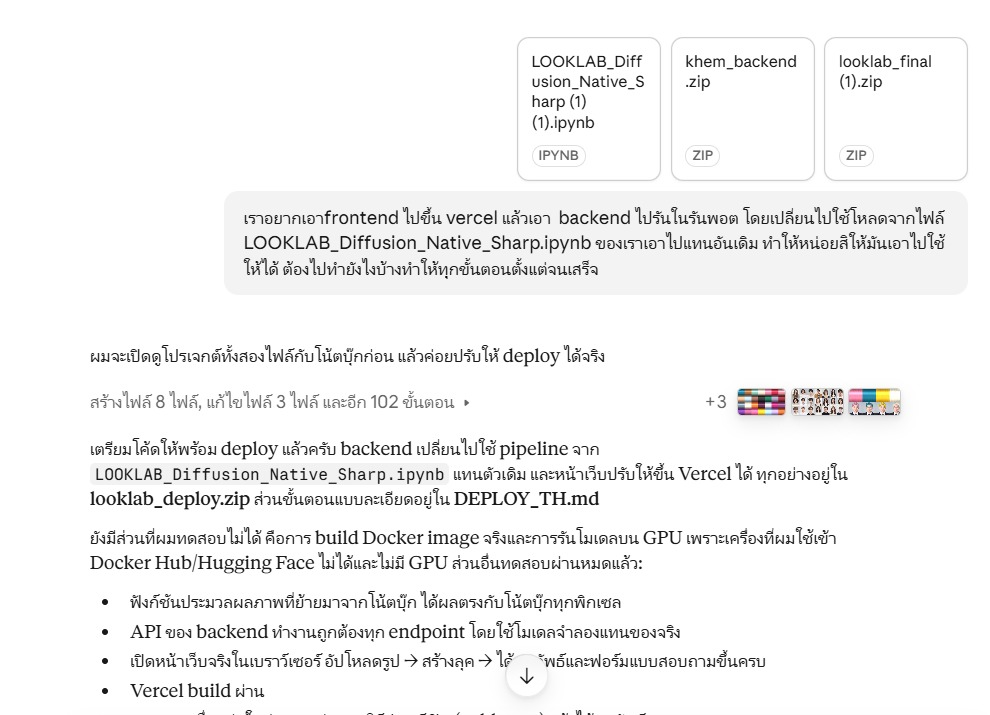
\includegraphics[width=0.65\textwidth]{images/ai_claude_deploy.jpg}
\caption{ข้อความสั่งงานและคำตอบของ Claude เรื่องการนำเว็บขึ้น Vercel และ RunPod}
\label{fig:ai_claude_deploy}
\end{figure}

\begin{figure}[H]
\centering
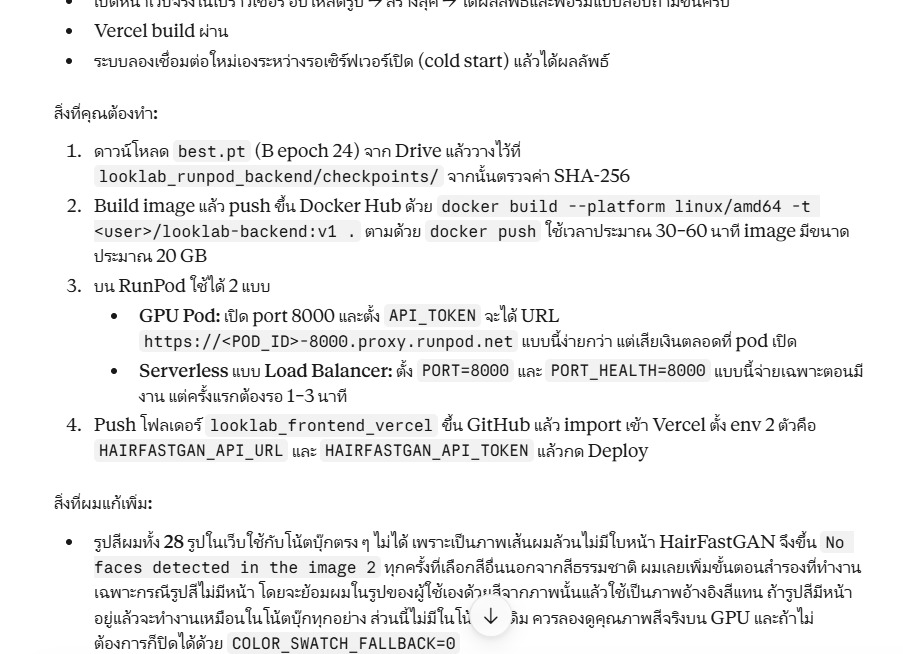
\includegraphics[width=0.65\textwidth]{images/ai_claude_steps.jpg}
\caption{ขั้นตอนที่ Claude ให้ผู้วิจัยทำต่อ และสิ่งที่ Claude แก้เพิ่ม}
\label{fig:ai_claude_steps}
\par\vspace{3pt}{\footnotesize\raggedright หมายเหตุ: GPU = Graphics Processing Unit (หน่วยประมวลผลกราฟิก), API = Application Programming Interface, SHA-256 = Secure Hash Algorithm 256 บิต (ค่าแฮชสำหรับตรวจไฟล์), env = Environment Variable (ตัวแปรสภาพแวดล้อม)\par}
\end{figure}

ผู้วิจัยใช้คำตอบนี้เป็นแนวทางหลักในการย้ายระบบ แต่ไม่ได้ใช้โค้ดทุกส่วนตามที่ได้มา
ตารางที่~\ref{tab:ai_deploy_compare} เทียบโค้ดหน้าเว็บที่ Claude ทำให้กับโค้ดหน้าเว็บที่ใช้จริงหลังย้ายขึ้น Vercel

\begin{table}[H]
\centering
\caption{เปรียบเทียบหน้าเว็บสำหรับ Vercel ที่ Claude ทำให้กับที่ใช้จริง}
\label{tab:ai_deploy_compare}
\small
\begin{tabular}{|L{3.4cm}|L{4.8cm}|L{4.8cm}|}
\hline
\textbf{รายการ} & \textbf{โค้ดจาก Claude} & \textbf{โค้ดที่ใช้จริง} \\ \hline
วิธีให้ \texttt{/api} ทำงานบน Vercel & เขียน Vercel Functions แยกไฟล์ใหม่แทน \texttt{server.ts} & รวม \texttt{server.ts} เดิมเป็น Function เดียวด้วยสคริปต์ตอน build \\ \hline
ที่เก็บ API key & ตัวแปรสภาพแวดล้อมฝั่ง Vercel & ตัวแปรสภาพแวดล้อมฝั่ง Vercel และเลิกรับ key จากเบราว์เซอร์ \\ \hline
การย่อรูปก่อนส่ง & ด้านยาวไม่เกิน 1,536 พิกเซล JPEG คุณภาพ 92\% & ใบหน้าไม่เกิน 1,600 พิกเซล รูปอ้างอิงไม่เกิน 1,408 พิกเซล JPEG คุณภาพ 92\% \\ \hline
รูปอ้างอิงสีผม & ภาพเส้นผมล้วน และย้อมผมในรูปผู้ใช้แทนเมื่อหาใบหน้าไม่เจอ & ภาพบุคคลที่เห็นใบหน้า 28 ภาพ ส่งให้ HairFastGAN ได้โดยตรง \\ \hline
การเชื่อมต่อแบบ ngrok & ปิดไว้ เปิดได้ด้วยตัวแปรสภาพแวดล้อม & นำออกทั้งหมด \\ \hline
\end{tabular}
\par\vspace{3pt}{\footnotesize\raggedright หมายเหตุ: API = Application Programming Interface, JPEG = Joint Photographic Experts Group (รูปแบบไฟล์ภาพ)\par}
\end{table}

สิ่งที่ผู้วิจัยใช้ตามคำตอบคือโครงสร้างการแยกหน้าเว็บไว้บน Vercel กับเซิร์ฟเวอร์โมเดลไว้บน RunPod แบบ Load Balancer
การเก็บ API key ไว้ฝั่งเซิร์ฟเวอร์ การย่อรูปก่อนส่งให้อยู่ในขีดจำกัดของ Vercel และการลองเชื่อมต่อใหม่ระหว่าง Cold Start
ส่วนที่ผู้วิจัยทำต่างไปมีสองเรื่อง
เรื่องแรก ผู้วิจัยไม่ได้ใช้ Vercel Functions ที่เขียนใหม่แยกไฟล์ แต่รวม \texttt{server.ts} ตัวเดิมเป็น Function เดียว
เพื่อให้หน้าเว็บบนเครื่องของผู้วิจัยและบน Vercel ใช้โค้ดเซิร์ฟเวอร์ชุดเดียวกัน
เรื่องที่สอง ผู้วิจัยไม่ได้ใช้ขั้นย้อมผมในรูปผู้ใช้ เพราะภาพที่ได้จะไม่ใช่ภาพอ้างอิงสีจริง
แต่เปลี่ยนรูปสีผมทั้ง 28 รูปเป็นภาพบุคคลที่เห็นใบหน้าชัด ซึ่งตรงกับวิธีที่ HairFastGAN ถูกออกแบบให้ใช้
ก่อนเปิดให้ทดลองใช้จริง ผู้วิจัยตรวจว่าหน้าเว็บบน Vercel เชื่อมกับเซิร์ฟเวอร์บน RunPod ได้
ลองสร้างภาพจากทั้งโหมดอัปโหลดและโหมดกล้อง และส่งแบบประเมินได้ครบ
นอกจากนี้ผู้วิจัยสร้าง API key ใหม่ตามที่ Claude เตือน และไม่นำไฟล์ \texttt{.env} ขึ้น GitHub

\section{สรุปการใช้คำตอบจาก AI}

ตารางที่~\ref{tab:ai_summary} สรุปคำถามทั้งสิบเอ็ดข้อ ข้อ 1--9 ถาม ChatGPT ข้อ 10 ใช้ Google AI Studio และข้อ 11 ถาม Claude คอลัมน์ ``สิ่งที่ AI ให้'' คือผลลัพธ์จากการถาม
คอลัมน์ ``การนำไปใช้'' บอกว่าผู้วิจัยใช้คำตอบแบบไหน และคอลัมน์สุดท้ายคือวิธีที่ผู้วิจัยใช้ตรวจสอบ
จะเห็นว่าไม่มีคำตอบข้อไหนที่ถูกนำไปใช้ทันทีโดยไม่ตรวจ
ทุกข้อผ่านการเทียบกับงานวิจัยต้นฉบับ โค้ดใน GitHub หรือผลการรันจริงก่อน

{\small
\begin{longtable}{|L{2.6cm}|L{3.6cm}|L{3.4cm}|L{3.6cm}|}
\caption{สรุปการใช้คำตอบจาก AI ในโครงงาน}\label{tab:ai_summary}\\
\hline
\textbf{คำถาม (AI ที่ใช้)} & \textbf{สิ่งที่ AI ให้} & \textbf{การนำไปใช้} & \textbf{วิธีตรวจสอบ} \\ \hline
\endfirsthead
\multicolumn{4}{l}{\footnotesize ตารางที่~\thetable\ (ต่อ)}\\
\hline
\textbf{คำถาม (AI ที่ใช้)} & \textbf{สิ่งที่ AI ให้} & \textbf{การนำไปใช้} & \textbf{วิธีตรวจสอบ} \\ \hline
\endhead
\multicolumn{4}{r}{\footnotesize ต่อหน้าถัดไป}\\
\endfoot
\multicolumn{4}{p{13.6cm}}{\footnotesize\raggedright หมายเหตุ: AI = Artificial Intelligence (ปัญญาประดิษฐ์), MUSIQ = Multi-scale Image Quality Transformer (คะแนนคุณภาพภาพ), ArcFace = โมเดลจดจำใบหน้าที่ใช้วัดความเหมือนของใบหน้า, IoU = Intersection over Union (สัดส่วนพื้นที่ผมที่ทับกัน)}\\
\endlastfoot
สร้าง Colab รัน HairFastGAN แบบ Pretrained (ChatGPT)
& สมุดบันทึกติดตั้ง ดาวน์โหลดน้ำหนัก และสร้างภาพ พร้อมคำอธิบายโมดูล
& ใช้เป็นจุดเริ่มต้น แล้วเขียนสมุดบันทึกสำหรับทดลองจริงขึ้นใหม่
& เทียบคำอธิบายกับงานวิจัยและโค้ด รันจริงบน Colab และไม่ใช้เวลาจากสมุดบันทึกนี้ \\ \hline
เพิ่มขั้นปรับภาพต่อจาก HairFastGAN (ChatGPT)
& เซลล์ Image-to-Image ความแรง 0.18 ค่านำทาง 3.5 ผสมกลับ 0.65
& เปลี่ยนวิธีเกือบทั้งหมด เป็น Inpainting เฉพาะผมกับใบหน้า ความแรง 0.15 ค่านำทาง 2.5
& ทดลองเทียบข้อความสั่งงาน วัดด้วย MUSIQ ArcFace IoU และความเห็นผู้ใช้ \\ \hline
วิเคราะห์ส่วนที่ปรับจูนได้ของ HairFastGAN (ChatGPT)
& คำอธิบายโมดูล คำแนะนำส่วนที่ควรปรับ การเตรียมข้อมูล และการแยกการปรับจูนจากการปรับค่า
& ใช้บางส่วน และปรับขอบเขต อัตราการเรียนรู้ และฟังก์ชันสูญเสียเอง
& ตรวจกับโค้ดจริง โหลดน้ำหนักด้วย \texttt{strict=True} และเลือก Checkpoint ด้วยชุดตรวจสอบ \\ \hline
สร้าง Colab รัน Barbershop แบบ Pretrained (ChatGPT)
& สมุดบันทึกล็อกรุ่นโค้ด ดาวน์โหลดน้ำหนัก และรันตามค่าเริ่มต้น พร้อมแก้โค้ดให้รันบน Colab ได้
& ใช้จำนวนรอบและการแก้โค้ดตามคำตอบ แล้วเพิ่มส่วนเก็บรหัสและจับเวลาเอง
& เทียบจำนวนรอบกับ \texttt{main.py} ตรวจว่าการแก้ไม่เปลี่ยนวิธีการ และรันจริง \\ \hline
เพิ่มขั้นปรับภาพต่อจาก Barbershop (ChatGPT)
& เซลล์ Image-to-Image ความแรง 0.15 ค่านำทาง 3.5 ผสมกลับ 0.70
& ไม่ใช้ค่าชุดนี้ ใช้ขั้นขัดเกลาชุดเดียวกับ HairFastGAN
& เทียบค่ากับคำตอบของ HairFastGAN แล้วพบว่าไม่เท่ากัน \\ \hline
วิเคราะห์ส่วนที่ปรับจูนได้ของ Barbershop (ChatGPT)
& อธิบายว่าโค้ดเดิมไม่ได้ฝึกน้ำหนัก เสนอทางเลือกการปรับจูน และแนะนำให้ปรับ StyleGAN2 ช่วงหลัง
& ใช้แนวทางปรับ StyleGAN2 ช่วงหลัง แต่ฝึกบนรหัสที่เก็บไว้
& ตรวจกับ \texttt{models/Net.py} และใช้ตัวสร้างภาพที่ปรับแล้วตลอดกระบวนการตอนทดสอบ \\ \hline
เปรียบเทียบ Barbershop A30 กับ HairFastGAN B24 (ChatGPT)
& ไฟล์เปรียบเทียบที่ตรวจน้ำหนัก A30 วัดผล 8 ภาพ แยกเวลา และอธิบายข้อจำกัดของตัวชี้วัด
& ใช้ตัวชี้วัดและการแยกเวลาตามไฟล์ รันกับภาพ 8 ชุด และตีความเป็นกรณีศึกษา
& เทียบค่าขั้นขัดเกลากับบทที่ 3 และนำตัวเลขจากไฟล์ผลลัพธ์โดยตรง \\ \hline
ออกแบบหน้าเว็บ LOOKLAB (ChatGPT)
& ภาพตัวอย่างหน้าเว็บ 10 แบบพร้อมชื่อและแนวสี
& เลือกแบบ 03 Peach Room เป็นแนวทาง ไม่ใช้ภาพตัวอย่างในเว็บ
& เทียบแบบกับลำดับการใช้งานของเว็บ \\ \hline
เขียนข้อความสั่งงานสำหรับ Google AI Studio (ChatGPT)
& ข้อความกำหนดสี การจัดวาง การแสดงผลบนมือถือ และให้รักษาฟังก์ชันเดิม
& ใช้ทั้งข้อความกับ Google AI Studio
& ใช้รายการฟังก์ชันในข้อความเป็นรายการตรวจผลในหัวข้อถัดไป \\ \hline
สร้างหน้าเว็บตามแบบที่เลือก (Google AI Studio)
& โค้ดหน้าเว็บใหม่ที่หน้าตาตรงแบบ แต่ตัดฟังก์ชันเดิมและจำลองผลเมื่อไม่มีเซิร์ฟเวอร์
& ไม่ใช้แทนโค้ดเดิม ใช้เฉพาะหน้าตาเป็นต้นแบบ
& เปิดโค้ดเทียบกับโปรเจกต์เดิมทีละส่วน \\ \hline
นำเว็บขึ้น Vercel และ RunPod (Claude)
& โค้ดเซิร์ฟเวอร์โมเดลสำหรับ RunPod โค้ดหน้าเว็บสำหรับ Vercel และคู่มือขั้นตอน
& ใช้โครงสร้างและการตั้งค่าตามคำตอบ แต่รวม \texttt{server.ts} เดิมเป็น Function เดียว และเปลี่ยนรูปสีผมแทนขั้นย้อมผม
& ทดลองสร้างภาพทั้งสองโหมดและส่งแบบประเมินบนเว็บจริงก่อนเปิดใช้ \\ \hline
\end{longtable}
}
